%% 
%% Copyright 2007-2020 Elsevier Ltd
%% 
%% This file is part of the 'Elsarticle Bundle'.
%% ---------------------------------------------
%% 
%% It may be distributed under the conditions of the LaTeX Project Public
%% License, either version 1.2 of this license or (at your option) any
%% later version.  The latest version of this license is in
%%    http://www.latex-project.org/lppl.txt
%% and version 1.2 or later is part of all distributions of LaTeX
%% version 1999/12/01 or later.
%% 
%% The list of all files belonging to the 'Elsarticle Bundle' is
%% given in the file `manifest.txt'.
%% 
%% Template article for Elsevier's document class `elsarticle'
%% with Harvard style bibliographic references

\documentclass[3p]{elsarticle}

%% Use the option review to obtain double line spacing
%% \documentclass[authoryear,preprint,review,12pt]{elsarticle}

%% Use the options 1p,twocolumn; 3p; 3p,twocolumn; 5p; or 5p,twocolumn
%% for a journal layout:
%% \documentclass[final,1p,times,authoryear]{elsarticle}
%% \documentclass[final,1p,times,twocolumn,authoryear]{elsarticle}
%% \documentclass[final,3p,times,authoryear]{elsarticle}
%% \documentclass[final,3p,times,twocolumn,authoryear]{elsarticle}
%% \documentclass[final,5p,times,authoryear]{elsarticle}
%% \documentclass[final,5p,times,twocolumn,authoryear]{elsarticle}

%% For including figures, graphicx.sty has been loaded in
%% elsarticle.cls. If you prefer to use the old commands
%% please give \usepackage{epsfig}

%% The amssymb package provides various useful mathematical symbols
\usepackage{amsmath}
\usepackage{caption}
\usepackage{subfig}
\usepackage{float}
\usepackage{booktabs}
\usepackage{tabularx}
\usepackage{amsfonts}
\usepackage{algorithm}
\usepackage{algorithmicx}
\usepackage{algpseudocode}
\usepackage{mathtools}
\usepackage{tikz}
\usepackage{subfig}
\usepackage{adjustbox}
\usepackage[figuresright]{rotating}
\usepackage{tikz}
\usepackage{multirow}
\usepackage{theorem}
\newtheorem{theorem}{Theorem}
\newtheorem{definition}{Definition}
\usepackage[hidelinks]{hyperref}
\usepackage{makecell}
\usepackage{calc}  % for '\widthof' macro
\usepackage{array} % for 'w' column type
\newtheorem{lemma}{Lemma}
\newtheorem{sublemma}{Lemma}[lemma]
\newlength\myleneiler
\newlength\mylenomega
\newenvironment{proof}{\paragraph{Proof:}}{\hfill$\square$}
\usetikzlibrary{shapes,arrows}
\tikzstyle{block} = [rectangle, draw, text width=4.5em, text centered, minimum height=4em]
\tikzstyle{line} = [draw, -latex']
\tikzstyle{decision} = [diamond, draw, text width=4.5em, text centered, inner sep=0pt]
\tikzstyle{cloud} = [draw, ellipse, text width=4.5em, text centered, minimum height=4em]
\usetikzlibrary{shapes, arrows.meta, positioning}
\tikzstyle{startstop} = [rectangle, rounded corners, minimum width=3cm, minimum height=1cm,text centered, draw=black, fill=red!30]
\tikzstyle{io} = [trapezium, trapezium left angle=70, trapezium right angle=110, minimum width=3cm, minimum height=1cm, text centered, draw=black, fill=blue!30]
\tikzstyle{process} = [rectangle, minimum width=3cm, minimum height=1cm, text centered, draw=black, fill=orange!30]
\tikzstyle{decision} = [diamond, minimum width=3cm, minimum height=1cm, text centered, draw=black, fill=green!30]
\tikzstyle{arrow} = [thick,->,>=stealth]
\setlength\myleneiler{(\widthof{Initial Condition (deg)}-4\tabcolsep)/3}
\setlength\mylenomega{(\widthof{Rotational Velocity Commands (rpm)}-4\tabcolsep)/4}
% \newcommand\highlightReference[1]{%
%   \expandafter\newcommand\csname highlightReference-#1\endcsname{}%
% }
% \let\oldbibitem\bibitem
% \def\bibitem#1 #2\par{%
%   \expandafter\ifx\csname highlightReference-#1\endcsname\relax
%     \oldbibitem{#1}#2\par
%   \else
%     \oldbibitem{#1}\highlight{#2}\par
%   \fi
% }
% \usepackage{color,soul}
% \newcommand\highlight[1]{\hl{#1}}

%% The amsthm package provides extended theorem environments
%% \usepackage{amsthm}

%% The lineno packages adds line numbers. Start line numbering with
%% \begin{linenumbers}, end it with \end{linenumbers}. Or switch it on
%% for the whole article with \linenumbers.
%% \usepackage{lineno}

%\journal{Franklin Institute}

\begin{document}

\begin{frontmatter}

%% Title, authors and addresses

%% use the tnoteref command within \title for footnotes;
%% use the tnotetext command for theassociated footnote;
%% use the fnref command within \author or \affiliation for footnotes;
%% use the fntext command for theassociated footnote;
%% use the corref command within \author for corresponding author footnotes;
%% use the cortext command for theassociated footnote;
%% use the ead command for the email address,
%% and the form \ead[url] for the home page:
%% \title{Title\tnoteref{label1}}
%% \tnotetext[label1]{}
%% \author{Name\corref{cor1}\fnref{label2}}
%% \ead{email address}
%% \ead[url]{home page}
%% \fntext[label2]{}
%% \cortext[cor1]{}
%% \affiliation{organization={},
%%            addressline={}, 
%%            city={},
%%            postcode={}, 
%%            state={},
%%            country={}}
%% \fntext[label3]{}

\title{Attitude Control of a 3-DoF Quadrotor Platform using a Linear Quadratic Integral Differential Game Approach}

%% use optional labels to link authors explicitly to addresses:
%% \author[label1,label2]{}
%% \affiliation[label1]{organization={},
%%             addressline={},
%%             city={},
%%             postcode={},
%%             state={},
%%             country={}}
%%
%% \affiliation[label2]{organization={},
%%             addressline={},
%%             city={},
%%             postcode={},
%%             state={},
%%             country={}}

%\author{Ali BaniAsad}
%\ead{ali.baniasad@ae.sharif.edu}
%\author{Alireza Sharifi \corref{cor1}}
%\ead{ar.sharifi@sharif.edu}
%\author{Reza Pordal}
%\ead{Reza.pordal77@student.sharif.edu}
%\cortext[cor1]{Corresponding author}

% \address{Department of Aerospace Engineering
% Sharif University of Technology Tehran, Iran}
% \address{Department of Aerospace Engineering
% Sharif University of Technology Tehran, Iran}
% \address{Department of Aerospace Engineering
% Sharif University of Technology Tehran, Iran}

%\author{Hadi Nobahari}
%\ead{nobahari@sharif.edu}


%\affiliation{organization={Department of Aerospace Engineering Sharif University of Technology},%Department and Organization
%            % addressline={}, 
%            city={Tehran},
%            % postcode={}, 
%            % state={},
%            country={Iran}}

\begin{abstract}
%% Text of abstract
    In this study, a linear quadratic integral differential game approach is applied to regulate and track the Euler angles for a quadrotor experimental platform using two players. %%%? long and hard to underestand.
    One produces commands for each channel of the quadrotor and
    another generates the worst disturbance based on the mini-maximization of a quadratic criterion with integral action.
    For this purpose, first, the attitude dynamics of the platform are modeled and its parameters are identified based on the Nonlinear Least Squares Trust-Region Reflective method.
    The performance of the proposed controller is evaluated for regulation and tracking problems.
    The ability of the controller is also examined in the disturbance rejection.
    Moreover, the influence of uncertainty modeling is studied on the obtained results.
    Then, the performance of the proposed controller is compared with the classic Proportional Integral Derivative, Linear Quadratic Regulator, and Linear Quadratic Integral Regulator. The results demonstrate the effectiveness of the Game Theory on the Linear Quadratic Regulator approach when the input disturbance occurs.
\end{abstract}

%%Graphical abstract
% \begin{graphicalabstract}
% %\includegraphics{grabs}
% \end{graphicalabstract}

%%Research highlights
% \begin{highlights}
% \item Research highlight 1
% \item Research highlight 2
% \end{highlights}

\begin{keyword}
%% keywords here, in the form: keyword \sep keyword

%% PACS codes here, in the form: \PACS code \sep code
Linear Quadratic Controller \sep~Differential Game Theory \sep~Quadrotor  \sep~3-DoF Experimental Platform \sep~Attitude Control. %%%? check --
%% MSC codes here, in the form: \MSC code \sep code
%% or \MSC[2008] code \sep code (2000 is the default)

\end{keyword}

\end{frontmatter}

%% \linenumbers

%% main text
\section{Introduction}\label{sec:intro}
% In this paper, an LQIR method, called LQIR-DG controller is suggested to produce the optimal and robust control command, i.e. rotational velocity command using the game theory approach.
% Since the LQIR-DG controller is affected by an exact model of the plant, the quadrotor's experimental platform is modeled and its parameters are identified based on experimental data. 
% For control purposes, its linear state-space form is extracted using linearization of the nonlinear UAV.
% then, the LQIR-DG technique is applied in real-time to the experimental platform.
% The performance of the LQIR-DG method is evaluated in the presence of the disturbance and modeling error for regulation and tracking purposes.
% A comparison is also performed between the results of classical PID, LQR, and LQIR and the proposed approach in real-time mode.
% The results show the proposed control structure is effective in the control of the quadrotor platform.

\noindent Quadrotors are a type of Vertical Unmanned Aerial Vehicle (VUAV), that have various applications such as investigation, strategic operation, optical sensing, and entertainment. The safe flight of the quadrotor in the presence of disturbances and mismodelling errors relies on a precise Attitude Control System (ACS). To regulate the quadrotor attitude, a Proportional Integral Derivative (PID) controller is utilized in~\cite{article_Abdul, article_Bolandi}. Due to the nonlinearity dynamics of the quadrotor, the PID strategy is not effective in the presence of disturbance and modeling error. To provide a faster control command in facing the modeling error and reduce the disturbance effect in the attitude control, the approaches such as Active Disturbance Rejection Control (ADRC)~\cite{CHENG2023}, nonlinear, and robust~\cite{DING2022580, CORTESROMERO202063} techniques can be found in the literatures.
ADRC is a model-free control technique used for systems with disturbances and unknown dynamics. In ref~\cite{WEI2022599}, ADRC method and a robust U-model active disturbance rejection control (RUADRC) have been proposed to reduce the phase lag and enhance the disturbance rejection ability. 

In the nonlinear control category, a Sliding Mode Control (SMC)~\cite{LABBADI2020290, MOFID2022455} law is applied based on the mathematical model of the plant and adopted for parameters perturbations. Moreover, this strategy is able to eliminate the disturbances of the system related to its high-gain feedback~\cite{YANG2021175}. In refs~\cite{WU2022436}, SMC method has been implemented to solve the nonlinear tracking problem for attitude control of the quadrotor, while the mismodelling error including time-varying mass has been considered. Moreover, in another strategy of nonlinear control, the intelligent approaches such as Reinforcement Learning (RL)~\cite{Hwangbo_2017, LIN2020135}, iterative learning~\cite{electronics10202474}, neural network~\cite{JIN202012241}, and fuzzy logic~\cite{GLIDA2022} have also been employed to control the attitude of the quadrotor. Besides, reinforcement learning has been utilized to train the control policy for the attitude of the quadrotor when the disturbance occurs~\cite{WANG2023222}.

The robust control strategy explicitly deals with parameters or disturbances. The robust algorithms can be categorized into two approaches: robust methods and robust control structures. The robust methods are utilized in linear and nonlinear control systems to achieve robust stability and/or performance in the presence of bounded modelling errors. In ref~\cite{MIRANDACOLORADO202047}, a Robust-PID strategy has been utilized to control the attitude dynamics of the quadrotor in presence of the aerodynamic disturbances like wind. In another approach such as H$_{\infty}$~\cite{WANG201910, REKABI202081} and $\mu$-synthesis~\cite{RODRIGUEZMARTINEZ2023739}, a minimaximization of the cost function including control effort and regulation performance have been utilized to produce the angular velocity commands for the attitude dynamics of the quadrotor while a worst-case scenario related to maximum uncertainty and disturbance is considered. 

In contrast with the policy of the robust control structure, the optimal control categories such as Linear Quadratic Gaussian (LQG)~\cite{7367782}, Linear Quadratic Regulator (LQR)~\cite{7064553_LQR}, Linear Quadratic Integral Regulator (LQIR)~\cite{article_LQIR}, and Model Predictive Controller (MPC)~\cite{SANTOS2022123, CAMARA20231} have been utilized to produce the optimal control commands for a quadrotor without considering the disturbance. Several methods with adding robust technique including Robust-LQR~\cite{robust_LQR}, Robust-LQG~\cite{XU202084}, Robust-MPC~\cite{YAN202335} and LQR-SMC can be found in the literature to reduce the disturbance effect. In another approach, the game theory technique is added to optimal control categories to provide a mathematical framework for analyzing decision-making in the presence of disturbance and modeling error. In this method, the control signals are produced using a pursuit-evasion game as well as the interactions and conflicts between two players are considered. The first player produces the control commands, and another player generates the worst disturbance based on the optimization of the desired objectives. An example of this category is the Linear Quadratic Regulator-Differential Game (LQR-DG) controller. The LQR-DG controller is implemented on a model of the ship~\cite{6957349}.



















































%  Quadrotors, a type of Vertical Unmanned Aerial Vehicle (VUAV), have found diverse applications in investigation, strategic operations, optical sensing, and entertainment. Precise control is crucial for the safe flight of quadrotors in the presence of disturbances. The Attitude Control System (ACS) plays a vital role in regulating the quadrotor's attitude, and the Proportional Integral Derivative (PID) controller has been commonly employed for this purpose in previous studies~\cite{article_Abdul, article_Bolandi}. However, due to the nonlinearity of the quadrotor dynamics, the PID strategy's effectiveness diminishes in the presence of disturbances and modeling errors.

% To address these challenges and enhance the quadrotor's attitude control, various model-based control strategies have been implemented on the ACS. These strategies encompass nonlinear control, intelligent control, optimal control, and robust control approaches.

% Nonlinear control methods such as Synergetic Control~\cite{article_Chara}, Feedback Linearization (FBL)~\cite{article_Aboudonia}. Sliding Mode Control (SMC)~\cite{LABBADI2020290, WU2022436, MOFID2022455, CHEN2022114, SRINIVASARAO2022516, ZHOU202185} have been utilized to regulate the quadrotor's Euler angles (roll, pitch, and yaw angles) intelligently.

% Intelligent control approaches, including reinforcement learning~\cite{Hwangbo_2017, LIN2020135, XIE2023477, WANG2023222}, iterative learning~\cite{electronics10202474}, machine learning~\cite{4564736}, and fuzzy logic~\cite{GLIDA2022}, have also been employed to control the attitude of the quadrotor.

% Optimal control strategies, such as Linear Quadratic Gaussian (LQG)~\cite{7367782}, Linear Quadratic Regulator (LQR)~\cite{7064553_LQR}, Linear Quadratic Integral Regulator (LQIR)~\cite{article_LQIR}, and Model Predictive Controller (MPC)~\cite{YAN202335, SANTOS2022123}, have been applied to generate optimal control commands for the quadrotor.

% In the domain of robust control, techniques like $H_{\infty}$ control~\cite{WANG201910, REKABI202081}, $\mu$-synthesis, and Linear Quadratic Regulator Differential Game (LQR-DG)~\cite{10025263} have been used to stabilize the quadrotor's Euler angles, considering worst-case scenarios and mini-maximization of a quadratic criterion, which includes control effort and regulation performance.

The implementation of the optimal control category based on the game theory still does not exist in any of the previous works. In this study, an LQR-DG method with an integral action is implemented as real-time on the 3-DoF experimental platform of the quadrotor to produce the robust control commands, i.e., rotational velocity of the quadrotor. Since this control strategy is a model-based method, first, the experimental platform of the quadrotor is modeled using the Newton-Euler formulation and its linear state-space form is derived. Then, the parameters of the quadrotor are estimated by matching experimental data with results from the model simulation. In the next step, the proposed controller is implemented on the Arduino Mega2560 board using the embedded coder platform in MATLAB and its performance is investigated in regulation and tracking problems. Moreover, the rejection capability of the input disturbance and modeling error is tested. Finally, a comparison is also performed between the results of classical PID, LQR, and LQIR with the proposed method. Moreover, the performance of the proposed structure has been investigated in flight and compared to the robust controller structures including ADRC and Disturbance Observer-Based Control (DOBC). The results demonstrate that this method has an excellent performance in the attitude control of the quadrotor platform. A demo video of the results is available online \href{https://youtu.be/SXZACxGaE1A?si=jxF7Uxh1Ed5-WX1J}{here}.


The innovation of this study mainly includes the following two aspects: (1) Proof of the proposed optimal-robust structure without steady-state error; For this purpose, first, the problem of an optimal control category based on the game theory approach with two players, one player tracks the best command, and the second player generates the input disturbance, is converted to the robust control problems. Then, an action integral is added to the linear quadratic regulator based on the game theory to eliminate the steady-state errors. Finally, proof of the proposed controller scheme based on the integral action is presented. (2) Implementation of the proposed optimal-robust structure; For this purpose, an optimal control strategy with integral action based on differential game theory is implemented on a 3-DOF quadrotor experimental setup. Then, the parameters of a quadrotor experimental setup have been identified with the experimental results. The performance of the proposed structure has been evaluated in flight and compared to the robust controller structures. Finally, the rejection capability of the input disturbance and modeling error is evaluated successfully.

% The remainder of this research is organized as follows: Section~\ref{sec:problem} presents the problem statement. Section~\ref{sec:modeling} outlines the dynamic platform modeling process. The proposed controller architecture is described in Section~\ref{sec:controller}. Section~\ref{sec:results} presents the numerical results, and Section~\ref{sec:conclusion} concludes the paper. A demo video showcasing the results is available online~\footnote{Demo video link: \url{https://drive.google.com/drive/folders/1DIJs3wmIpmwI8slyHeitA6Ebe-khKTCt?usp=share_link}}.

This research is organized as follows: section~\ref{sec:problem} presents the problem statement.
In section~\ref{sec:modeling}, the dynamic platform is modeled. Then, the presented controller architecture is denoted in section~\ref{sec:controller}. 
In sections~\ref{sec:results} and~\ref{sec:conclusion}, numerical results and a conclusion are represented, respectively.

\section{Problem Statement}\label{sec:problem}
\noindent The experimental quadrotor platform rotates freely with rotational velocity ($\Omega_i, i = 1, 2, 3, 4$) about its roll, pitch, and yaw axes, according to Figure~\ref{fig:quadrotor}.
The angular velocities in the body frame $(p, q, r)$ and the Euler angles $(\phi, \theta, \psi)$ are measured using an Attitude Heading Reference System (AHRS).
The measured states are utilized in the structure of the proposed controller to stabilize the quadrotor platform.
The graphical abstract of the LQIR-DG controller strategy is depicted in Figure~\ref{fig:blockdiagram}.
\begin{figure}[H]
    \centering
    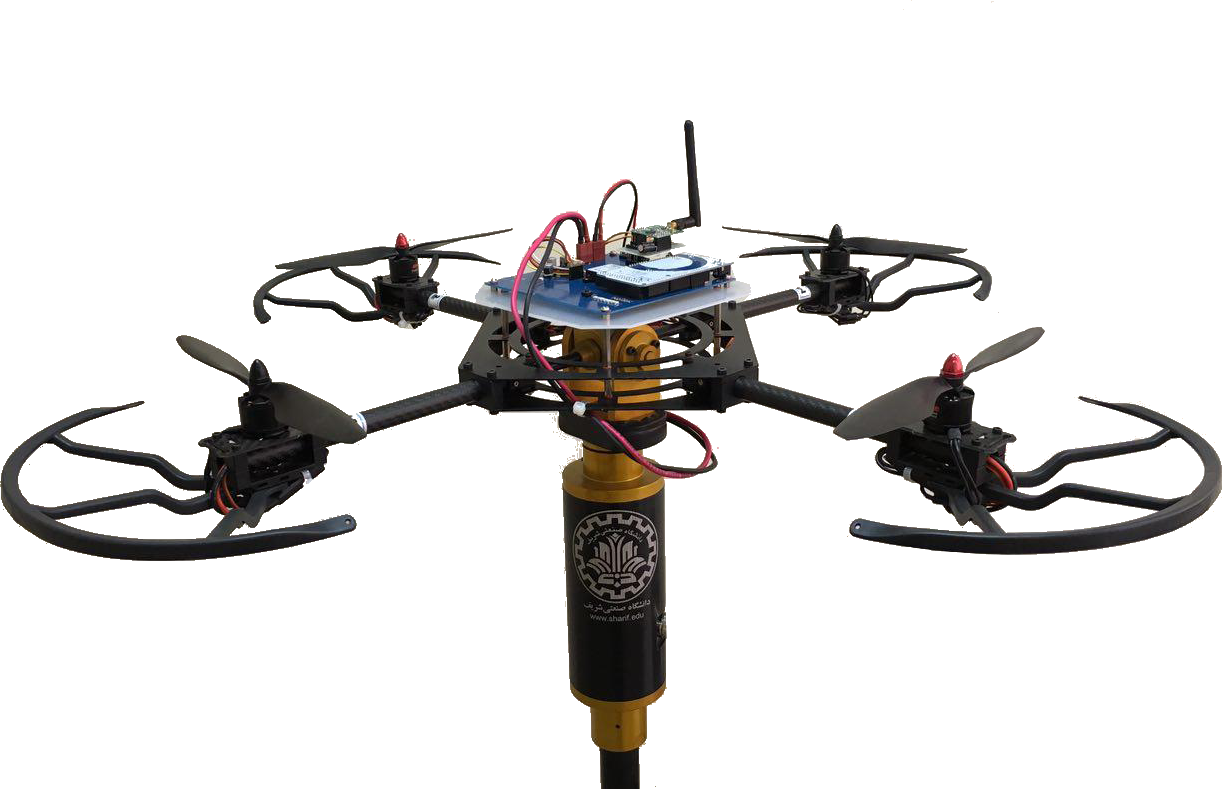
\includegraphics[width=0.7\textwidth]{../Figure/3DOFQuad.png}
    \caption{3-DoF Quadrotor platform.}
~\label{fig:quadrotor}
 \end{figure}
 
 \begin{figure}[H]
    \centering
    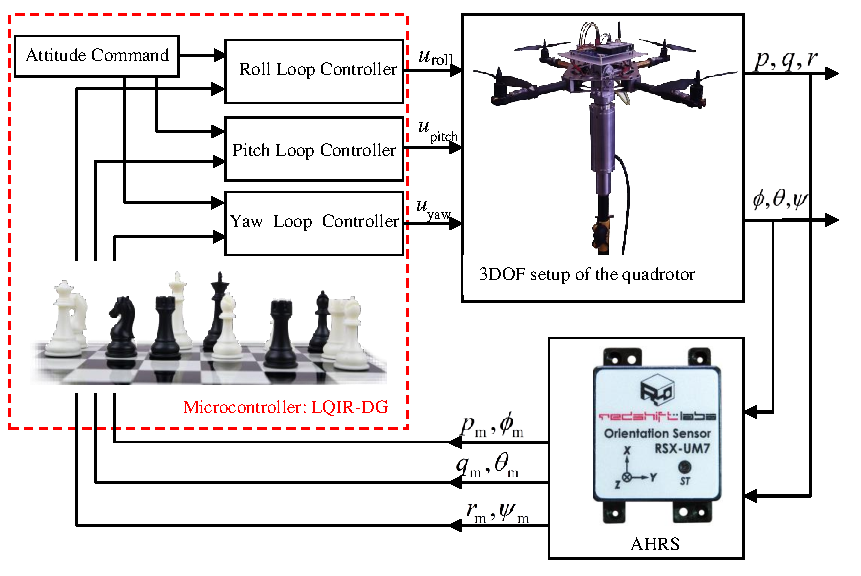
\includegraphics[width=0.7\textwidth]{../Figure/schematic.pdf}
    \caption{Graphical abstract of the LQIR-DG controller.}
~\label{fig:blockdiagram}
 \end{figure}
 \section{Model of the Quadrotor Platform}\label{sec:modeling}
 \noindent Here, the quadrotor platform is modeled as nonlinear.
 Then, a state-space model and a linear model are developed for control purposes to be utilized in the controller strategy.
 Finally, a nonlinear identification method is applied to identify the parameters of the quadrotor.
 \subsection{Quadrotor Configuration}
 \noindent According to Figure\ref{fig:schematic}, the 3-DoF quadrotor schematic is including four rotors rotating the $z_B$ axis in the body frame with a rotational velocity, $\Omega_i~(i=1, 2, 3, 4)$. To eliminate the yawing moment, rotors (2, 4) and (1, 3) rotate clockwise and counter counterclockwise, respectively.

% \noindent Figure~\ref{fig:schematic} shows the quadrotor schematic. It depicts four rotors rotating around the $z_B$ axis in the coordinate system of the body. The rotors have a rotational velocity of $\Omega_r$.
% The quadrotor platform has 3 degrees of freedom, including roll, pitch, and yaw motions, which are described by roll $(\phi)$, pitch $(\theta)$, and yaw $(\psi)$ angles, respectively. %%%? two roll, pitch, yaw
% To counteract the yawing moment, rotors 1 and 3 rotate counterclockwise, while rotors 2 and 4 rotate clockwise. This configuration is designed to cancel out the torque generated by the propellers and stabilize the quadrotor platform. %%%? write by my self and hace many similarity
\begin{figure}[H]
    \centering
    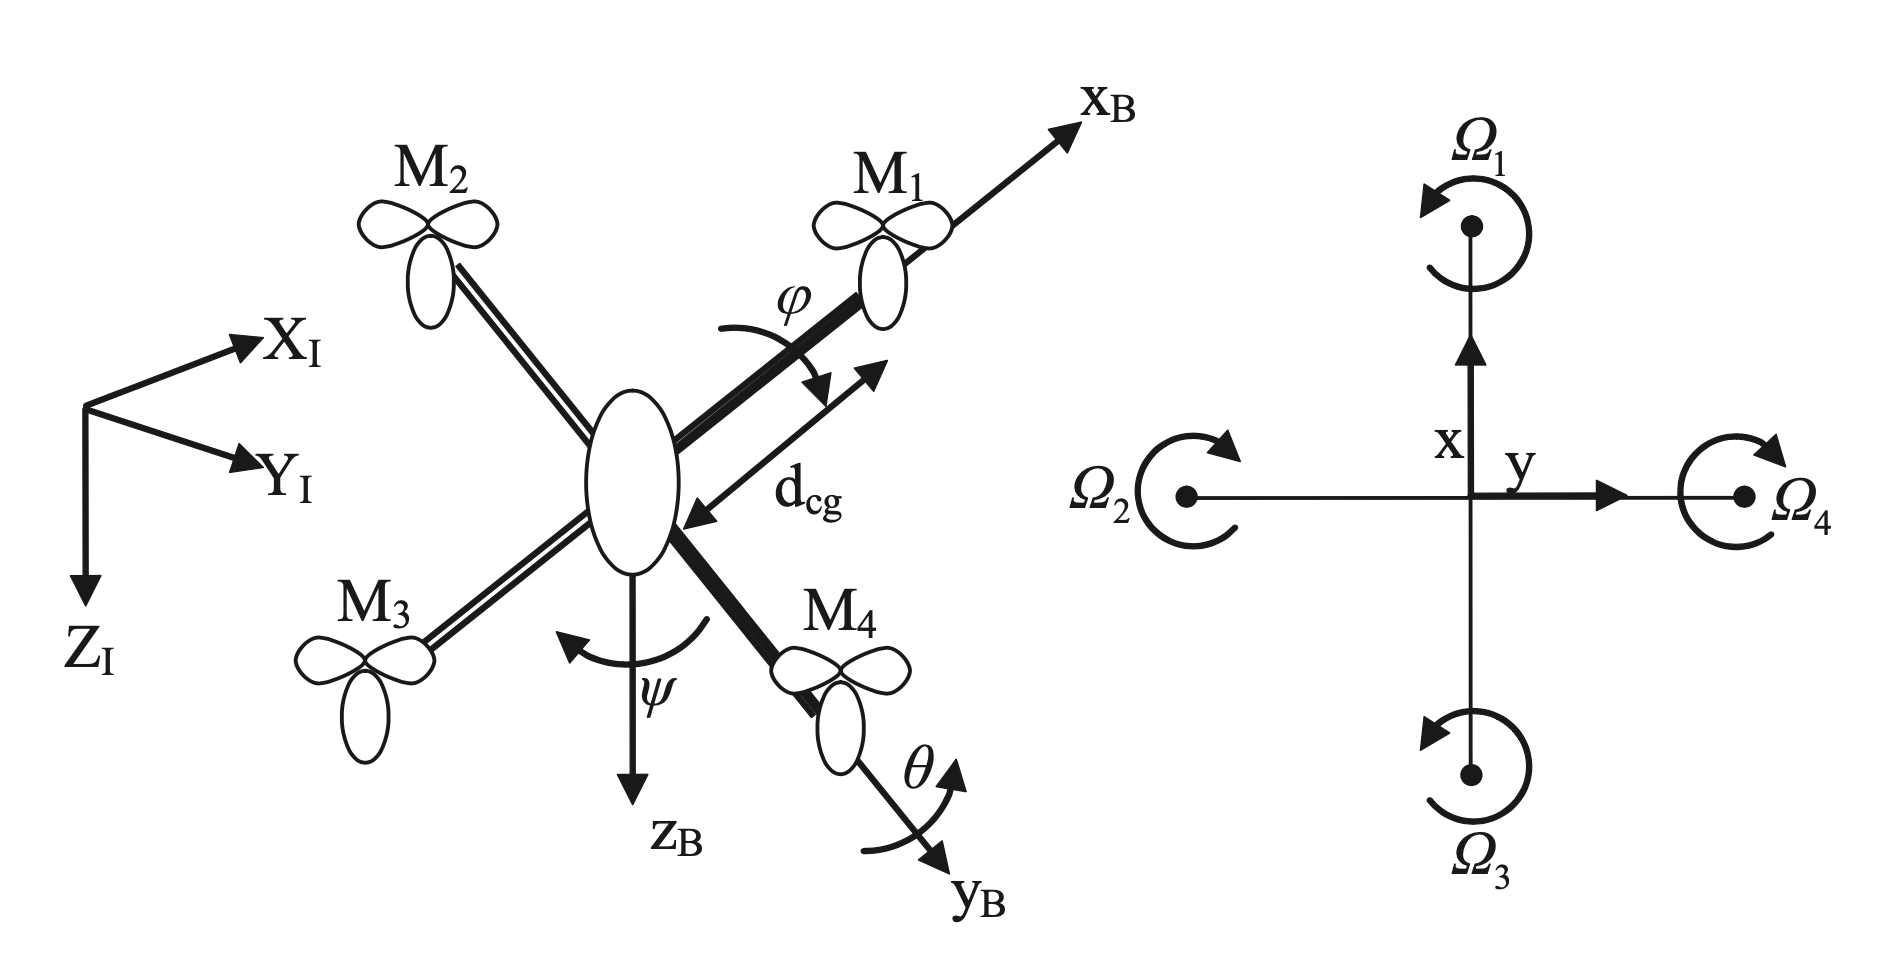
\includegraphics[width=12cm]{../Figure/schematic.png}
    \caption{Quadrotor configuration.}
~\label{fig:schematic}
\end{figure}
\subsection{Dynamic Modeling of the Quadrotor Platform}
\noindent Here, according to Newton-Euler, the model of the quadrotor platform is presented as follows~\cite{4399042, article_Bouabdallah}:
% \begin{equation}
%     \begin{bmatrix}
%         \dot p \\
%         \dot q \\
%         \dot r
%     \end{bmatrix} = \begin{bmatrix}
%         \dfrac{J_z}{\Gamma} & 0 & \dfrac{J_{xy}}{\Gamma} \\
%         0 & \dfrac{1}{J_y} & 0 \\
%         \dfrac{J_{xy}}{\Gamma} & 0 & \dfrac{J_x}{\Gamma}
%     \end{bmatrix} \left(
%         \begin{bmatrix}
%             0 & r & -q \\
%             -r & 0 & p \\
%             q & -p & 0
%         \end{bmatrix}\begin{bmatrix}
%             J_x & 0 & -J_{xy} \\
%             0 & J_y & 0 \\
%             -J_{xy} & 0 & J_z
%         \end{bmatrix} +
%         \begin{bmatrix}
%             u_{\text{roll}} \\
%             u_{\text{pitch}} \\
%             u_{\text{yaw}}
%         \end{bmatrix} + \begin{bmatrix}
%             d_{\text{roll}} \\
%             d_{\text{pitch}} \\
%             d_{\text{yaw}}
%         \end{bmatrix}
%     \right)
% \end{equation}

% \begin{equation}
%     \begin{bmatrix}
%     \dot{p} \\
%     \dot{q} \\
%     \dot{r}
%     \end{bmatrix} = \frac{1}{\Gamma} \begin{bmatrix}
%     J_z & 0 & J_{xy} \\
%     0 & \frac{\Gamma}{J_y} & 0 \\
%     J_{xy} & 0 & J_x
%     \end{bmatrix} \left(
%     \begin{bmatrix}
%     0 & r & -q \\
%     -r & 0 & p \\
%     q & -p & 0
%     \end{bmatrix} \begin{bmatrix}
%     J_x & 0 & -J_{xy} \\
%     0 & J_y & 0 \\
%     -J_{xy} & 0 & J_z
%     \end{bmatrix} +
%     \begin{bmatrix}
%     u_{\text{roll}} \\
%     u_{\text{pitch}} \\
%     u_{\text{yaw}}
%     \end{bmatrix} + \begin{bmatrix}
%     d_{\text{roll}} \\
%     d_{\text{pitch}} \\
%     d_{\text{yaw}}
%     \end{bmatrix}
%     \right).
% \end{equation}

% \begin{align*}
%   \begin{bmatrix}
%   \dot{p} \\
%   \dot{q} \\
%   \dot{r}
%   \end{bmatrix} = \frac{1}{\Gamma} \begin{bmatrix}
%   J_z & 0 & J_{xy} \\
%   0 & \frac{\Gamma}{J_y} & 0 \\
%   J_{xy} & 0 & J_x
%   \end{bmatrix} \left(&
%   \begin{bmatrix}
%   0 & r & -q \\
%   -r & 0 & p \\
%   q & -p & 0
%   \end{bmatrix} \begin{bmatrix}
%   J_x & 0 & -J_{xy} \\
%   0 & J_y & 0 \\
%   -J_{xy} & 0 & J_z
%   \end{bmatrix} +\right. \\
%   \left.&
%   \begin{bmatrix}
%   \mathrm{b\,d}_{\text{cg}} (\Omega_{c, 2}^2 - \Omega_{c, 4}^2) \\
%   \mathrm{b\,d}_{\text{cg}} (\Omega_{c, 1}^2 - \Omega_{c, 3}^2) \\
%   \mathrm{d} (\Omega_{c, 1}^2 - \Omega_{c, 2}^2 + \Omega_{c, 3}^2 - \Omega_{c, 4}^2)
%   \end{bmatrix}& + \begin{bmatrix}
%   d_{\text{roll}} \\
%   d_{\text{pitch}} \\
%   d_{\text{yaw}}
%   \end{bmatrix}
%   \right)
% \end{align*}

% \begin{align*}
%     \begin{bmatrix}
%         \dot{p} \\
%         \dot{q} \\
%         \dot{r}
%     \end{bmatrix} &= \frac{1}{\Gamma} \begin{bmatrix}
%         J_z & 0 & J_{xy} \\
%         0 & \frac{\Gamma}{J_y} & 0 \\
%         J_{xy} & 0 & J_x
%     \end{bmatrix} \left(
%         \begin{bmatrix}
%             0 & r & -q \\
%             -r & 0 & p \\
%             q & -p & 0
%         \end{bmatrix} \begin{bmatrix}
%             J_x & 0 & -J_{xy} \\
%             0 & J_y & 0 \\
%             -J_{xy} & 0 & J_z
%         \end{bmatrix} +
%         \begin{bmatrix}
%             \mathrm{b\,d}_{\text{cg}} (\Omega_{c, 2}^2 - \Omega_{c, 4}^2) \\
%             \mathrm{b\,d}_{\text{cg}} (\Omega_{c, 1}^2 - \Omega_{c, 3}^2) \\
%             \mathrm{d} (\Omega_{c, 1}^2 - \Omega_{c, 2}^2 + \Omega_{c, 3}^2 - \Omega_{c, 4}^2)
%         \end{bmatrix} +
%         \begin{bmatrix}
%             d_{\text{roll}} \\
%             d_{\text{pitch}} \\
%             d_{\text{yaw}}
%         \end{bmatrix}
%     \right)
% \end{align*}

% \begin{equation}
%     \begin{aligned}
%         \begin{bmatrix}
%             \dot{p} \\
%             \dot{q} \\
%             \dot{r}
%         \end{bmatrix} = \frac{1}{\Gamma} \begin{bmatrix}
%             J_z & 0 & J_{xy} \\
%             0 & \frac{\Gamma}{J_y} & 0 \\
%             J_{xy} & 0 & J_x
%         \end{bmatrix} \Bigg(
%         &\begin{bmatrix}
%             0 & r & -q \\
%             -r & 0 & p \\
%             q & -p & 0
%         \end{bmatrix} \begin{bmatrix}
%             J_x & 0 & -J_{xy} \\
%             0 & J_y & 0 \\
%             -J_{xy} & 0 & J_z
%         \end{bmatrix} \\
%         \quad+ &\begin{bmatrix}
%             \mathrm{b\,d}_{\text{cg}} (\Omega_{c, 2}^2 - \Omega_{c, 4}^2) \\
%             \mathrm{b\,d}_{\text{cg}} (\Omega_{c, 1}^2 - \Omega_{c, 3}^2) \\
%             \mathrm{d} (\Omega_{c, 1}^2 - \Omega_{c, 2}^2 + \Omega_{c, 3}^2 - \Omega_{c, 4}^2)
%         \end{bmatrix} + \begin{bmatrix}
%             d_{\text{roll}} \\
%             d_{\text{pitch}} \\
%             d_{\text{yaw}}
%         \end{bmatrix}
%         \Bigg)
%     \end{aligned}
% \end{equation}

%%%%%%%%%%%%%%%% J must be text and x and y %%%%%%%%%%%%%%%%%

% \begin{align}
%     \dot p = \mathrm{\Gamma}_1pq - \mathrm{\Gamma}_2qr+ \mathrm{\Gamma}_3(\Omega_{c, 2}^2 - \Omega_{c, 4}^2) + \mathrm{\Gamma}_4\mathrm{d} (\Omega_{c, 1}^2 - \Omega_{c, 2}^2 + \Omega_{c, 3}^2 - \Omega_{c, 4}^2) + \mathrm{\Gamma}_5\Omega_{c, r} + \mathrm{\Gamma}_3d_{\text{yaw}} + \mathrm{\Gamma}_4d_{\text{yaw}} \\
%     \dot q = \mathrm{\Gamma}_6pr - \mathrm{\Gamma}_7(p^2 - r^2) + \mathrm{\Gamma}_8(\Omega_{c, 1}^2 - \Omega_{c, 3}^2) + \mathrm{\Gamma}_9\Omega_{c, r} + \mathrm{\Gamma}_8d_{\text{pitch}}\\
%     \dot r = \mathrm{\Gamma}_{10}pq - \mathrm{\Gamma}_{1}qr + \mathrm{\Gamma}_{11}(\Omega_{c, 1}^2 - \Omega_{c, 2}^2 + \Omega_{c, 3}^2 - \Omega_{c, 4}^2) + \mathrm{\Gamma}_{4}\mathrm{d} (\Omega_{c, 2}^2 - \Omega_{c, 4}^2) + \mathrm{\Gamma}_{11}d_{\text{roll}} + \mathrm{\Gamma}_{4}d_{\text{yaw}}
% \end{align}


\begin{align}
    \dot{p} &= \Gamma_1 pq - \Gamma_2 qr + \Gamma_3 \mathrm{b}\mathrm{d}_{\text{cg}} (\Omega_{c, 2}^2 - \Omega_{c, 4}^2) + \Gamma_4 \mathrm{d} (\Omega_{c, 1}^2 - \Omega_{c, 2}^2 + \Omega_{c, 3}^2 - \Omega_{c, 4}^2) + \Gamma_5 q \Omega_{c, r} + \Gamma_3 d_{\text{roll}} + \Gamma_4 d_{\text{yaw}} \\
    \dot{q} &= \Gamma_6 pr - \Gamma_7 (p^2 - r^2) + \Gamma_8  \mathrm{b}\mathrm{d}_{\text{cg}}(\Omega_{c, 1}^2 - \Omega_{c, 3}^2) + \Gamma_9 p \Omega_{c, r} + \Gamma_8 d_{\text{pitch}} \\
    \dot{r} &= \Gamma_{10} pq - \Gamma_{1} qr + \Gamma_{11} (\Omega_{c, 1}^2 - \Omega_{c, 2}^2 + \Omega_{c, 3}^2 - \Omega_{c, 4}^2) + \Gamma_{4}  \mathrm{b}\mathrm{d}_{\text{cg}} (\Omega_{c, 2}^2 - \Omega_{c, 4}^2) + \Gamma_{11} d_{\text{roll}} + \Gamma_{4} d_{\text{yaw}}
\end{align}
% \begin{align}
% &\dot p = \dfrac{\mathrm{I}_{\text{yy}} - \mathrm{I}_{\text{zz}}}
% {\mathrm{I}_{\text{xx}}} qr + q \dfrac{\mathrm{I}_{\text{rotor}}}
% {\mathrm{I}_{\text{xx}}}\Omega_{c, r} + \dfrac{\mathrm{b\,d}_{\text{cg}} (\Omega_{c, 2}^2 - \Omega_{c, 4}^2)}{\mathrm{I}
% _{\text{xx}}} + \dfrac{d_{\text{roll}}}{\mathrm{I}_{\text{xx}}}
% \\
% &\dot q = \dfrac{\mathrm{I}_{\text{zz}} - 
% \mathrm{I}_{\text{xx}}}{\mathrm{I}_{\text{yy}}} rp -
% p \dfrac{\mathrm{I}_{\text{rotor}}}{\mathrm{I}_{\text{yy}}}\Omega_{c, r} + 
% \dfrac{\mathrm{b\,d}_{\text{cg}} (\Omega_{c, 1}^2 - \Omega_{c, 3}^2)}{\mathrm{I}_{\text{yy}}} +
% \dfrac{d_{\text{pitch}}}{\mathrm{I}_{\text{yy}}}
% \\
% &\dot r = \dfrac{\mathrm{I}_{\text{xx}} -
% \mathrm{I}_{\text{yy}}}{\mathrm{I}_{\text{zz}}} pq 
% +  \dfrac{\mathrm{d} (\Omega_{c, 1}^2 - \Omega_{c, 2}^2 + \Omega_{c, 3}^2 - \Omega_{c, 4}^2)}{\mathrm{I}_{\text{zz}}} 
% + \dfrac{d_{\text{yaw}}}{\mathrm{I}_{\text{zz}}}
% \end{align}
In the above equations, $\Gamma_i (i = 1, \ldots, 8)$ is defined as
\begin{equation}
    \begin{aligned}
        \Gamma_1 &= \dfrac{\mathrm{I}_{\text{xz}}\left(\mathrm{I}_{\text{xx}} - \mathrm{I}_{\text{yy}} + \mathrm{I}_{\text{zz}}\right)}{\mathrm{\Gamma}}, & \Gamma_2 &= \dfrac{\mathrm{I}_{\text{zz}}\left(\mathrm{I}_{\text{zz}} - \mathrm{I}_{\text{yy}}\right)+\mathrm{I}_{\text{xz}}^2}{\mathrm{\Gamma}}, & \Gamma_3 &= \dfrac{\mathrm{I}_{\text{zz}}}{\mathrm{\Gamma}}, & \Gamma_4 &= \dfrac{\mathrm{I}_{\text{xz}}}{\mathrm{\Gamma}} \\
        \Gamma_5 &= \dfrac{\mathrm{I}_{\text{rotor}}}{\mathrm{I}_{\text{xx}}}, & \Gamma_6 &= \dfrac{\mathrm{I}_{\text{zz}}-\mathrm{I}_{\text{xx}}}{\mathrm{I}_{\text{yy}}}, & \Gamma_7 &= \dfrac{\mathrm{I}_{\text{xz}}}{\mathrm{I}_{\text{yy}}}, & \Gamma_8 &= \dfrac{1}{\mathrm{I}_{\text{yy}}} \\
        \Gamma_9 &= \dfrac{\mathrm{I}_{\text{rotor}}}{\mathrm{I}_{\text{yy}}}, & \Gamma_{10} &= \dfrac{\left(\mathrm{I}_{\text{xx}}-\mathrm{I}_{\text{yy}}\right)+\mathrm{I}_{\text{xz}}^2}{\mathrm{\Gamma}}, & \Gamma_{11} &= \dfrac{\mathrm{I}_{\text{xx}}}{\mathrm{\Gamma}} & &
    \end{aligned}
\end{equation}
Moreover $\Gamma = \mathrm{J}_{\text{x}}\mathrm{J}_{\text{z}} - \mathrm{J}_{\text{xy}}^2$.
where $\Omega_{c, i}~(i=1, 2, 3, 4)$ is the rotational velocity, computed as
 \begin{align}
    \Omega_{c, 1}^2 &= \Omega_{\text{mean}}^2 + \dfrac{1}{2\mathrm{b\,d}_{\text{cg}}}u_{\text{pitch}} + \dfrac{1}{4d}u_{\text{yaw}} \\
    \Omega_{c, 2}^2 &= \Omega_{\text{mean}}^2 + \dfrac{1}{2\mathrm{b\,d}_{\text{cg}}}u_{\text{roll}} - \dfrac{1}{4d}u_{\text{yaw}}\\
    \Omega_{c, 3}^2 &= \Omega_{\text{mean}}^2 - \dfrac{1}{2\mathrm{b\,d}_{\text{cg}}}u_{\text{pitch}} + \dfrac{1}{4d}u_{\text{yaw}} \\
    \Omega_{c, 4}^2 &= \Omega_{\text{mean}}^2 - \dfrac{1}{2\mathrm{b\,d}_{\text{cg}}}u_{\text{roll}} - \dfrac{1}{4d}u_{\text{yaw}}
\end{align}

In the above equation, $\Omega_{\text{mean}}$ is the rotational velocity of the rotors. Also, $\mathrm{d}_{\text{cg}}$, $\text{d}$, and $\text{b}$ represent the distance between the rotors and the gravity center, drag factor, and thrust factor, respectively.
$d_{\text{roll}}$, $d_{\text{pitch}}$, and $d_{\text{yaw}}$ denote the disturbances produced in the body coordinate frame. Additionally,
$u_{\text{roll}}$, $u_{\text{pitch}}$, and $u_{\text{yaw}}$ are control commands generated by the LQIR-DG controller.
%  $\mathrm{I}_{\text{rotor}}$ is rotor inertia, and 
 $\mathrm{I}_{\text{xx}}$, $\mathrm{I}_{\text{yy}}$, and $\mathrm{I}_{\text{zz}}$ are the moments of inertia.
Euler angle rates are also determined from angular body rates as follows:
\begin{equation}
    \begin{bmatrix}
    \dot\phi \\
    \dot\theta \\
    \dot\psi
    \end{bmatrix} = 
    \begin{bmatrix}
    1 & \sin(\phi)\tan(\theta) & \cos(\phi)\tan(\theta) \\
    0 & \cos(\phi) & -\sin(\phi) \\
    0 & \sin(\phi)/\cos(\theta) & \cos(\phi)/\cos(\theta)
    \end{bmatrix}
    \begin{bmatrix}
    p \\
    q \\
    r
    \end{bmatrix}
\end{equation}
% The residual rotor velocity, denoted by $\Omega_{c,r}$, is calculated as follows:
% \begin{equation}
%   \Omega_{c, r} = -\Omega_{c, 1} + \Omega_{c, 2} - \Omega_{c, 3} + \Omega_{c, 4}
% \end{equation}

\subsection{State-Space Formulation}\label{sec:state-space}
\noindent By defining $\boldsymbol{\mathrm{x}}_{\text{roll}} = \begin{bmatrix}
    x_1 & x_2
\end{bmatrix}^{\mathrm{T}}=
\begin{bmatrix}
    p & \phi
\end{bmatrix}^{\mathrm{T}}$
,
$\boldsymbol{\mathrm{x}}_{\text{pitch}} = \begin{bmatrix}
    x_3 & x_4 \end{bmatrix}^{\mathrm{T}} = 
    \begin{bmatrix}
    q & \theta \end{bmatrix}^{\mathrm{T}}
    $
    , and
    $\boldsymbol{\mathrm{x}}_{\text{yaw}} = 
    \begin{bmatrix}
        x_5 & x_6
    \end{bmatrix}^{\mathrm{T}} = 
    \begin{bmatrix}
        r & \psi
    \end{bmatrix}^{\mathrm{T}}$, as well as by considering the control inputs as 
    $\boldsymbol{u} = \begin{bmatrix}
        u_{\text{roll}} & u_{\text{roll}} & u_{\text{roll}}
    \end{bmatrix} = \\ \begin{bmatrix}
        \mathrm{b\,d}_{\text{cg}}(\Omega_{c, 2}^2 - \Omega_{c, 4}^2) & \mathrm{b\,d}_{\text{cg}}(\Omega_{c, 1}^2 - \Omega_{c, 3}^2) &
        \mathrm{b\,d}_{\text{cg}}(\Omega_{c, 1}^2 - \Omega_{c, 2}^2+ \Omega_{c, 3}^2 - \Omega_{c, 4}^2)
    \end{bmatrix}$.
    The nonlinear model of the quadrotor platform in the state-space form $\dot{\boldsymbol{x}} = \boldsymbol{f}(\boldsymbol{x}, \boldsymbol{u})$ is presented as follows:
% \begin{align}\label{eq:diffeq}
%     \dot x_1 &= \Gamma_1x_3 x_5 + \Gamma_2 x_3 \Omega_r + \Gamma_3\mathrm{b\,d}_{\text{cg}} (\Omega_{c, 2}^2 - \Omega_{c, 4}^2) + \Gamma_3d_{\text{roll}} \\[0.5em]
%     \dot x_2 &= x_1 + (x_3\sin(x_2) + x_3\cos(x_2))\tan(x_4)
%     \\[0.5em]
%     \dot x_3 &= \Gamma_4 x_1 x_5 - \Gamma_5 x_1 \Omega_r +  \Gamma_6\mathrm{b\,d}_{\text{cg}} (\Omega_{c, 1}^2 - \Omega_{c, 3}^2) + \Gamma_6d_{\text{pitch}}\\[0.5em]~\label{eq:diffeq-mid}
%     \dot x_4 &= x_3\cos(x_4) - x_5\sin(x_2)\\[0.5em]
%     \dot x_5 &= \Gamma_7x_1 x_3 +  \Gamma_8\mathrm{d} (\Omega_{c, 1}^2 - \Omega_{c, 2}^2 + \Omega_{c, 3}^2 - \Omega_{c, 4}^2) + \Gamma_8d_{\text{yaw}}\\[0.5em] 
%     \dot x_6 &= (x_3\sin(x_4) + x_5\cos(x_2))/\cos(x_4)~\label{eq:diffeq-end}
% \end{align}
% where $\Gamma_i (i = 1, \ldots, 8)$ is defined as
% \begin{equation}
%     \begin{split}
%         \Gamma_1 &= \dfrac{\mathrm{I}_{\text{yy}} - \mathrm{I}_{\text{zz}}}{\mathrm{I}_{\text{xx}}}, \quad \Gamma_2 = \dfrac{\mathrm{I}_{\text{rotor}}}{\mathrm{I}_{\text{xx}}}, \quad \Gamma_3 = \dfrac{1}{\mathrm{I}_{\text{xx}}}\\ \Gamma_4 &= \dfrac{\mathrm{I}_{\text{zz}} - \mathrm{I}_{\text{xx}}}{\mathrm{I}_{\text{yy}}}, \quad \Gamma_5 = \dfrac{\mathrm{I}_{\text{rotor}}}{\mathrm{I}_{\text{yy}}}, \quad \Gamma_6 = \dfrac{1}{\mathrm{I}_{\text{yy}}} \\ \Gamma_7 &= \dfrac{\mathrm{I}_{\text{xx}} - \mathrm{I}_{\text{yy}}}{\mathrm{I}_{\text{zz}}}, \quad \Gamma_8 = \dfrac{1}{\mathrm{I}_{\text{zz}}}
%     \end{split}
% \end{equation}
% \begin{align}
%     \dot{x}_1 &= \Gamma_1 x_1 x_3 - \Gamma_2 x_3 x_5 + \Gamma_3 (\Omega_{c, 2}^2 - \Omega_{c, 4}^2) + \Gamma_4 \mathrm{d} (\Omega_{c, 1}^2 - \Omega_{c, 2}^2 + \Omega_{c, 3}^2 - \Omega_{c, 4}^2) + \Gamma_5 \Omega_{c, r} + \Gamma_3 d_{\text{roll}} + \Gamma_4 d_{\text{yaw}} \\
%     \dot x_2 &= x_1 + (x_3\sin(x_2) + x_3\cos(x_2))\tan(x_4)\\
%     \dot{x}_3 &= \Gamma_6 x_1 x_5 - \Gamma_7 (x_1^2 - x_5^2) + \Gamma_8 (\Omega_{c, 1}^2 - \Omega_{c, 3}^2) + \Gamma_9 \Omega_{c, r} + \Gamma_8 d_{\text{pitch}} \\
%     \dot x_4 &= x_3\cos(x_4) - x_5\sin(x_2)\\
%     \dot{x}_5 &= \Gamma_{10} x_1 x_3 - \Gamma_{1} x_3 x_5 + \Gamma_{11} (\Omega_{c, 1}^2 - \Omega_{c, 2}^2 + \Omega_{c, 3}^2 - \Omega_{c, 4}^2) + \Gamma_{4} \mathrm{d} (\Omega_{c, 2}^2 - \Omega_{c, 4}^2) + \Gamma_{11} d_{\text{yaw}} + \Gamma_{4} d_{\text{roll}}\\
%     \dot x_6 &= (x_3\sin(x_4) + x_5\cos(x_2))/\cos(x_4)~\label{eq:eq_of_motion_end1}
% \end{align}
\begin{align}
    f_1 = \dot{x}_1 &= \Gamma_1 x_1 x_3 - \Gamma_2 x_3 x_5 + \Gamma_3  (u_{\text{roll}} + d_{\text{roll}})
 + \Gamma_4  (u_{\text{yaw}} + u_{\text{yaw}}) 
+ \Gamma_5 x_3\Omega_{c, r}  \label{eq:eq_of_motion_start1} \\
    f_2 = \dot{x}_2 &= x_1 + (x_3\sin(x_2) + x_5\cos(x_2))\tan(x_4)  \\
    f_3 = \dot{x}_3 &= \Gamma_6 x_1 x_5 - \Gamma_7 (x_1^2 - x_5^2) + \Gamma_8  (u_{\text{pitch}} + d_{\text{pitch}})- \Gamma_9 x_1 \Omega_{c, r} \\
    f_4 = \dot{x}_4 &= x_3\cos(x_2) - x_5\sin(x_2) \\
    f_5 = \dot{x}_5 &= \Gamma_{10} x_1 x_3 - \Gamma_{1} x_3 x_5 + \Gamma_{11} (u_{\text{yaw}} + d_{\text{yaw}}) + \Gamma_{4}(u_{\text{roll}} + d_{\text{roll}})\\
    f_6 = \dot{x}_6 &= \dfrac{x_3\sin(x_2) + x_5\cos(x_2)}{\cos(x_4)}~\label{eq:eq_of_motion_end1}
\end{align}


% \begin{align}
%     \dot x_1& = \Gamma_1x_1x_3 - \Gamma_2x_3x_5 + \Gamma_3 \mathrm{b\,d}_{\text{cg}} (\Omega_{c, 2}^2 - \Omega_{c, 4}^2) + \Gamma_4\mathrm{d} (\Omega_{c, 1}^2 - \Omega_{c, 2}^2 + \Omega_{c, 3}^2 - \Omega_{c, 4}^2)+\Gamma_3d_{\text{roll}}\\[2mm]~\label{eq:eq_of_motion_start1}
%     \dot x_2 &= x_1 + (x_3\sin(x_2) + x_3\cos(x_2))\tan(x_4)\\
%     \dot x_3 &= \Gamma_5x_1x_5 - \Gamma_6(x_1^2-x_5^2) + \dfrac{1}{J_y}\mathrm{b\,d}_{\text{cg}} (\Omega_{c, 1}^2 - \Omega_{c, 3}^2)+ \dfrac{1}{J_y}d_{\text{pitch}}\\
%     \dot x_4 &= x_3\cos(x_4) - x_5\sin(x_2)\\[2mm]
%     \dot x_5 &= \Gamma_7x_1x_3 - \Gamma_1x_3x_5 + \Gamma_4\mathrm{b\,d}_{\text{cg}} (\Omega_{c, 2}^2 - \Omega_{c, 4}^2)+\Gamma_8\mathrm{d} (\Omega_{c, 1}^2 - \Omega_{c, 2}^2 + \Omega_{c, 3}^2 - \Omega_{c, 4}^2)+\Gamma_8d_{\text{yaw}}\\[2mm]
%     \dot x_6 &= (x_3\sin(x_4) + x_5\cos(x_2))/\cos(x_4)~\label{eq:eq_of_motion_end1}
% \end{align}
% where $\Gamma_i (i = 1, \ldots, 8)$ is defined as
% \begin{equation}
%     \begin{aligned}
%         \Gamma_1 &= \dfrac{J_{xz}(J_x-J_y+J_z)}{\Gamma}, & \Gamma_2 &= \dfrac{J_z(J_z-J_y)+J_{xz}^2}{\Gamma}, & \Gamma_3 &= \dfrac{J_z}{\Gamma}, \\
%         \Gamma_4 &= \dfrac{J_{xz}}{\Gamma}, & \Gamma_5 &= \dfrac{J_z-J_x}{J_y}, & \Gamma_6 &= \dfrac{J_{xz}}{J_y}, \\
%         \Gamma_7 &= \dfrac{J_x(J_x-J_y)+J_{xz}^2}{\Gamma}, & \Gamma_8 &= \dfrac{J_x}{\Gamma}.
%     \end{aligned}
% \end{equation}
    

The measurement vector, obtained from the AHRS, is presented as follows:
\begin{equation}
    \begin{split}
        \boldsymbol{\mathrm{z}} &= \begin{bmatrix}
        p \
        q \
        r \
        \phi \
        \theta \
        \psi
    \end{bmatrix}^\mathrm{T} + \boldsymbol{\nu}
    \end{split}
\end{equation}
where $\boldsymbol{\nu}$ is a Gaussian white noise. Moreover, the superscripts $\mathrm{T}$ indicate the transpose notation.
%%%? capital or small G g ? 
\subsection{Linear Model}

\noindent By defining $\boldsymbol{\dot{\mathrm{x}}} = \begin{bmatrix}
    \boldsymbol{{\mathrm{\dot x_{\text{roll}}}}}&
    \boldsymbol{{\mathrm{\dot x_{\text{pitch}}}}}&
    \boldsymbol{{\mathrm{\dot x_{\text{yaw}}}}}
\end{bmatrix}^{\mathrm{T}}$, the linear model of the quadrotor platform represented about the equilibrium points $(\boldsymbol{{\mathrm{x}}}_e^*\!=\!0$ and $\boldsymbol{{\mathrm{u}}}_e^*\!=\!0)$ as
\begin{equation}\label{eq:linear}
    \boldsymbol{\dot{\mathrm{x}}} = \boldsymbol{\mathrm{A\,x}} + 
    \boldsymbol{\mathrm{B}}
    \left(\boldsymbol{\mathrm{u}} + \boldsymbol{\mathrm{d}}\right)
\end{equation}
where $\boldsymbol{\mathrm{d}} = \text{diag}([d_{\text{roll}}, d_{\text{pitch}}, d_{\text{yaw}}])$ denotes the input disturbance.
$\boldsymbol{\mathrm{A}}$ is the dynamic system matrix, denoted as
\begin{equation}
    \boldsymbol{\mathrm{A}} = \begin{bmatrix}
        \boldsymbol{{\mathrm{A_{\text{roll}}}}} & \boldsymbol{0} & \boldsymbol{0}\\
        \boldsymbol{0} & \boldsymbol{{\mathrm{A_{\text{pitch}}}}} & \boldsymbol{0} \\
        \boldsymbol{0} & \boldsymbol{0} & \boldsymbol{{\mathrm{A_{\text{yaw}}}}}
    \end{bmatrix}
\end{equation}
$
        \boldsymbol{\mathrm{A}}_{\text{roll}}  =\boldsymbol{\mathrm{A}}_{\text{pitch}}  = \boldsymbol{\mathrm{A}}_{\text{yaw}}  = \begin{bmatrix}
            0 & 0\\
            1 & 0
        \end{bmatrix}
$. Also, $\boldsymbol{\mathrm{B}}$ is the input matrix defined as
\begin{equation}
    \boldsymbol{\mathrm{B}} = 
     \begin{bmatrix}
        \Gamma_3 & 0 & \Gamma_4\\
        0 & 0 & 0 \\
        0 & \Gamma_8 & 0 \\
        0 & 0 & 0 \\
        \Gamma_4 & 0 & \Gamma_{11} \\
        0 & 0 & 0
    \end{bmatrix}
\end{equation}
% \begin{equation}
%     \boldsymbol{\mathrm{B}} =
%     \begin{bmatrix}
%         \boldsymbol{{\mathrm{B_{\text{roll}}}}} & \boldsymbol{0} & \boldsymbol{0}\\
%         \boldsymbol{0} & \boldsymbol{{\mathrm{B_{\text{pitch}}}}} & \boldsymbol{0} \\
%         \boldsymbol{0} & \boldsymbol{0} & \boldsymbol{{\mathrm{B_{\text{yaw}}}}}
%     \end{bmatrix}
% \end{equation}
% where $\boldsymbol{\mathrm{B}}_{\text{roll}}  = \begin{bmatrix}
%     \dfrac{1}{\Gamma_3}
%     &
%     0
% \end{bmatrix}^{\mathrm{T}}$, $\boldsymbol{\mathrm{B}}_{\text{pitch}}  = \begin{bmatrix}
%     \dfrac{1}{\mathrm{I}_{\text{yy}}}
%     &
%     0
% \end{bmatrix}^{\mathrm{T}}$, and $\boldsymbol{\mathrm{B}}_{\text{yaw}}  = \begin{bmatrix}
%     \dfrac{1}{\Gamma_8}
%     &
%     0
% \end{bmatrix}^{\mathrm{T}}$.
\subsection{Identification of the Platform Parameters}
\noindent In this section, the Nonlinear Least Squares (NLS) algorithm is utilized for estimating the model parameters ($\boldsymbol{\mathrm{\Gamma}}$) of the 3-DoF experimental platform using experimental data.
This technique is based on the Trust-Region Reflective (TRR) method, which finds the best values for $\boldsymbol{\mathrm{\Gamma}}$ by minimizing a cost function, defined as
\begin{equation}
    \min_{\Gamma}\left(\parallel e(\Gamma) \parallel^2\right) = 
    \min_{\Gamma} \left(\sum_{j=1}^{n}(\boldsymbol{z}_j- \tilde{\boldsymbol{z}}_j)(\boldsymbol{z}_j- \tilde{\boldsymbol{z}}_j)^\mathrm{T}\right)
\end{equation} %%%? what is j ??
where $\boldsymbol{z}$ and $\tilde{\boldsymbol{z}}$ are the experimental and simulated output signals when the same input signals are applied.
Moreover, $n$ is the number of scenarios.
To find a vector $\Gamma$, the optimization process performs until convergence is achieved. %%%?
The structure of the identification approach is illustrated in figure~\ref{fig:identification}.

\begin{figure}[H]
    \centering
    \resizebox{1\textwidth}{!}{
    \begin{tikzpicture}[font=\small,thick]
        % Start block
        \node[draw, align=center,       minimum width=2.5cm,        minimum height=1cm, fill=blue!10] (block1) {\textbf{Experimental Data} \\Input: rotational velocity\\
        Output: attitude};
            
        % Voltage and Current Measurement
        \node[draw, align=center,       below=of block1,        minimum width=3.5cm,        minimum height=1cm, fill=blue!10    ] (block2) {\textbf{Data Preprocessing} \\ Synchronization experimental, vs simulated data.};
        
        % Power and voltage variation
        
        \node[draw, align=center,       below=of block2,        minimum width=3.5cm,        minimum height=1cm, fill=blue!10    ] (block3) {\textbf{NLS-TRR Optimization}\\
        Set bounds for parameters\\
        The set initial seed for all parameters\\
        Minimization of the cost function.};

        \node[draw, align=center,   below right=of block3,  minimum width=3cm,  minimum height=2.5cm,   fill=green!10   ] (block_p) {{Identified parameters}\\
        $\boldsymbol\Gamma = \begin{bmatrix}\Gamma_1 &
            \Gamma_2 & \Gamma_3 & \Gamma_4\\
            \Gamma_5 & \Gamma_6 & \Gamma_7 & \Gamma_8
        \end{bmatrix}$};

        \node[draw, align=center,   below left=of block3,   minimum width=3cm,  minimum height=2.5cm,   fill=red!10 ] (block_s) {{simulated model}\\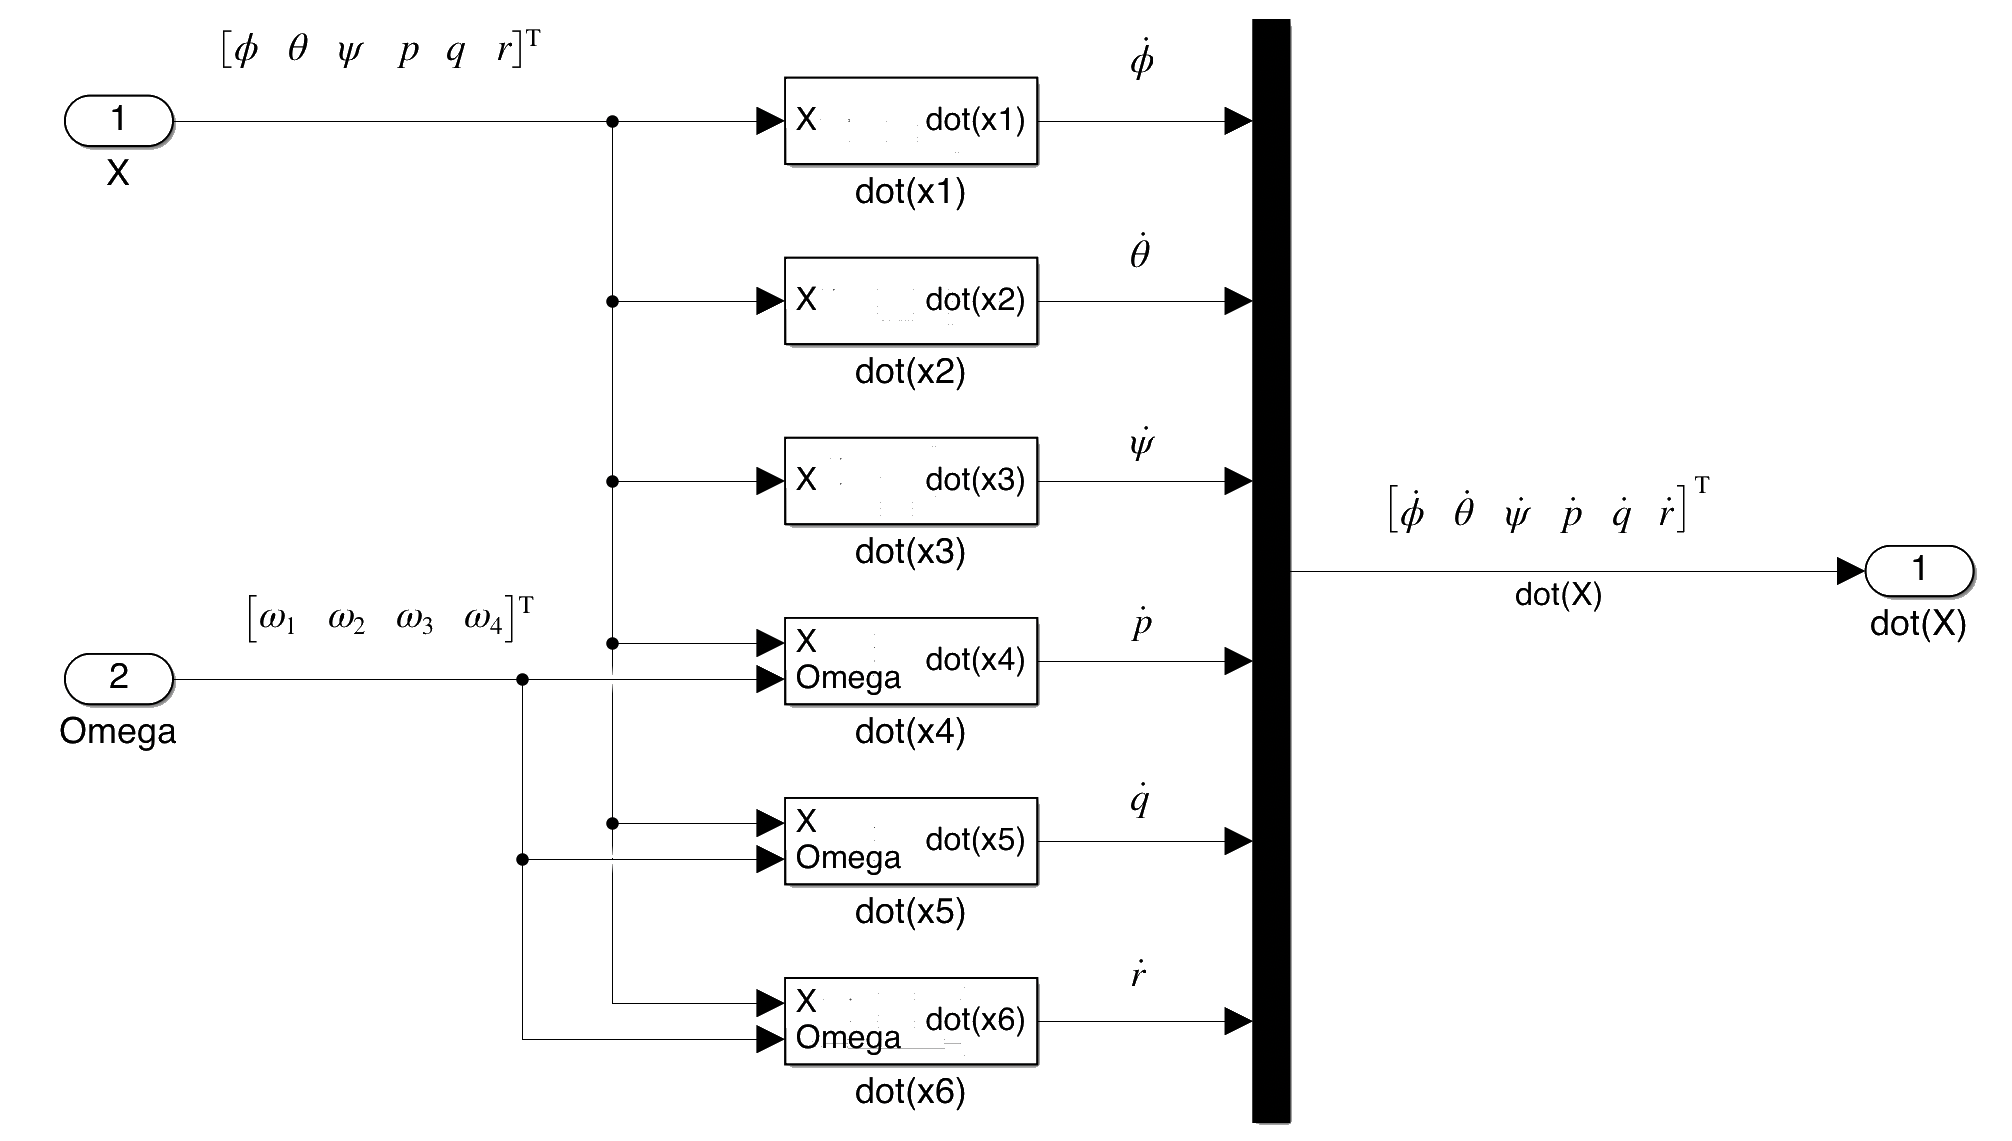
\includegraphics[scale=.05]{../Figure/All-six.png}};
        
        % Conditions test
        \node[draw,     diamond,        below =4cm of block3,       minimum width=2.5cm,        inner sep=0,        fill=yellow!10  ] (block4) { Error $< \delta$};
        
        \node[draw,     below=1.5cm of block4,      minimum height=1cm,     minimum width=2.5cm,        inner sep=0,        fill=blue!10    ] (block5) {End};
        
        \node[draw,     right=2cm of block4,        minimum height=1cm,     minimum width=2.5cm,        fill=red!10     ] (block6) {Insufficient experimental data};
                
         
         
        % Arrows
        \draw[-latex] (block1) edge (block2)
            (block2) edge (block3)
            (block3) -| (block_s);
            % (block3) edge (block_p);
    
        \draw[-latex] (block3) -| (block_p);
    
        \draw[-latex] (block_s) -| (block4);
    
        \draw[-latex] (block_p) -| (block4);
    
        \draw[stealth-stealth] (block_s) -- (block_p);
         
        \draw[-latex] (block4) -- (block5)
            node[pos=0.5,fill=white,inner sep=0]{Yes};
         
        \draw[-latex] (block4) -- (block6)
            node[pos=0.5,fill=white,inner sep=0]{No};
    
        \coordinate[left=5.5cm of block3] (aux);
        \coordinate[right= of block_p] (aux1);
        % \draw[-latex] (block6) |- (block2);
        \draw[-latex] (block1) -| (aux) |- (block4);
        \draw[-latex] (block6) -| (aux1) |- (block1);
        \end{tikzpicture}
        }
        \caption{Structure of TRRLS identification approach.}
        \label{fig:identification}
\end{figure}
\section{LQIR-DG Controller Structure}\label{sec:controller}
\noindent First, the augmented states of the quadrotor platform, including the states and their integrals are selected to use in the structure of the LQIR-DG controller for eliminating the steady-state errors. Then, the design methodology of the controller structure is introduced to produce the best commands for the 3-DoF quadrotor platform.
\subsection{Augmented States}
\noindent To augment an integral action into the control strategy architecture, the augmented states are defined as $\boldsymbol{\mathrm{x}}_{a} = \begin{bmatrix}
    \boldsymbol{\mathrm{x}} &
    \displaystyle\int\boldsymbol{\mathrm{x}}
\end{bmatrix}^\mathrm{T}$. Then, the quadrotor platform model, utilized in the controller structure, is presented as

\begin{equation}\label{systemlqidg}
    \begin{split}
        \boldsymbol{\dot{\mathrm{x}}}_a &= \mathbf{A}_a \boldsymbol{\mathrm{x}}_a + \mathbf{B}_a
         \left(\boldsymbol{\mathrm{u}} + \boldsymbol{\mathrm{d}}\right)%, \quad \boldsymbol{x}(0) = 
    \end{split}
\end{equation}
where $\mathbf{A}_a = \begin{bmatrix}
\boldsymbol{\mathrm{A}} & \boldsymbol{0}\\
\boldsymbol{\mathrm{I}} & \boldsymbol{0}
\end{bmatrix}$ and $\mathbf{B}_a=\begin{bmatrix}
    \boldsymbol{\mathrm{B}}\\
    \boldsymbol{0}
\end{bmatrix}$.
The notation $\boldsymbol{\mathrm{I}}$ denotes the identity matrix.
\subsection{LQIR-DG Control Scheme with Integral Action}
\noindent In the proposed controller scheme, two fundamental players are selected in accordance with the game theory approach. The primary player determines the control commands, while another player generates the worst possible disturbance.
To achieve the primary objective, the first player minimizes the following cost function but the other player maximizes it:
\begin{equation}\label{eq:min_max_cost_function}
    \min_{u} \max_{d} J(\boldsymbol{\mathrm{x}}_{\textrm{a}_i}, {d_i}, {u_i})= \min_{d} \max_{u}
     \int_{0}^{\mathrm{t_f}}\biggl (\boldsymbol{\mathrm{x}}^\mathrm{T}_{\textrm{a}_i}  \boldsymbol{\mathrm{Q}}_i \boldsymbol{\mathrm{x}}_{\textrm{a}_i}+
    {{u^\mathrm{T}_i}}  {{R}} {{u_i}}-
    {{d^\mathrm{T}_{i}}} {{ R_{d} d_{i}}}
    \biggl )\mathrm{d}t
\end{equation}
where $\mathrm{t_f}$ is the stop time and $i$-index denotes the roll, pitch, and yaw channels of the quadrotor. $\boldsymbol{\mathrm{Q_i}}$, ${{R_{d}}}$, and ${{R}}$ are weight coefficients of the cost function.
By solving the above problem, the optimal control command is computed as follows~\cite{LQDG}:
\begin{equation}
    {{u_i}} = -\boldsymbol{{\mathrm{K}}}_{i} \boldsymbol{{\mathrm{x}}}_{\textrm{a}_i}
\end{equation}
Moreover, the worst disturbance is obtained as
\begin{equation}
    {{d_i}} =\boldsymbol{{\mathrm{K}}}_{\textrm{d}_i}\boldsymbol{{\mathrm{x}}}_{\mathrm{a}_i}
\end{equation}
Here, $\boldsymbol{{\mathrm{K_{d_i}}}}$ and $\boldsymbol{{\mathrm{K_i}}}$ are gain values defined as follows:
\begin{align}
    \boldsymbol{{\mathrm{K}}}_{\textrm{d}_i} &= {{{R}}^{-1}_{d}}\boldsymbol{{\mathrm{B}}}_{\mathrm{a}_{i}}^\mathrm{T}\boldsymbol{{\mathrm{P}}}_{\mathrm{a}_{i}}\\
    \boldsymbol{{\mathrm{K}}}_{i} &= {{{R}}^{-1}}
    \boldsymbol{{\mathrm{B}}}_{\mathrm{a}_{i}}^\mathrm{T}
    \boldsymbol{{\mathrm{P}}}_{\mathrm{a}_{i}}
\end{align}
$\boldsymbol{{\mathrm{P}}}_{\mathrm{a}_{i}}$ satisfy
\begin{align}\label{coupled_riccatti_LQIDG}
    -\mathbf{A}^\mathrm{T}\mathbf{P}_{\mathrm{a}_{i}} - \mathbf{P}_{\mathrm{a}_{i}}\mathbf{A} + \mathbf{P}_{\mathrm{a}_{i}}(\mathbf{S}_{\mathrm{a}_i} - \mathbf{S}_{\mathrm{a_d}_i}) \mathbf{P}_{\mathrm{a}_{i}} - \mathbf{Q}_{i} = 0 
\end{align}
 where $\mathbf{S}_{\mathrm{a}_i} = \mathbf{B}_{\mathrm{a}_i}{R}^{-1}\mathbf{B}_{\mathrm{a}_i}^\mathrm{T}$ and $\mathbf{S}_{\mathrm{a_d}_i} = \mathbf{B}_{\mathrm{a}_i}{R}_d^{-1}\mathbf{B}_{\mathrm{a}_i}^\mathrm{T}$

% where $\mathbf{S}_{\mathrm{a}_i} = \mathbf{B}_{\mathrm{a}_i}\mathbf{R}^{-1}\mathbf{B}_{\mathrm{a}_i}^\mathrm{T}$ and $\mathbf{S}_{\mathrm{a_d}_i} = \mathbf{B}_{\mathrm{a}_i}\mathbf{R}_d^{-1}\mathbf{B}_{\mathrm{a}_i}^\mathrm{T}$. Therefore, $\mathbf{P}_{\mathrm{a}_i} = -\mathbf{P}_{\mathrm{a}_{d_i}}$ and two Ricatti equations have a following solution:

% \begin{equation}

% \end{equation}

% subsection for tunning weighta with TCACS optimization
% \subsection{TCACS Optimization for Tuning the Weighting Matrices}
% \noindent To optimize the weighting matrix of the LQIR-DG (Linear Quadratic Integral Regulator with Disturbance Rejection) controller, the TCACS (Tabu Continuous Ant Colony System)~\cite{10.1007/978-3-540-28646-2_27} optimization method was utilized. The objective was to tune the controller parameters for improved performance in a 3-degree-of-freedom simulation.

% In the optimization process, the cost function was formulated based on the LQIR-DG controller, where the state feedback matrix $\boldsymbol{\mathrm{Q}}$ and the disturbance rejection matrix $R_d$ were the key parameters to be determined. To simplify the problem, it was assumed that R (the penalty matrix for control inputs) was fixed at a value of 1.

% By employing the TCACS optimization method, the algorithm explored the search space to find the optimal values of $\boldsymbol{\mathrm{Q}}$ and $R_d$ for each channel. The objective was to achieve a balance between control effort and disturbance rejection while ensuring stable and robust control performance.

% The optimization process aimed to fine-tune the controller parameters for the specific dynamics of the system under consideration. The resulting weighting matrices $\boldsymbol{\mathrm{Q}}$ and $R_d$ would enable the LQIR-DG controller to efficiently regulate the system while effectively rejecting disturbances in the simulation.
% \noindent In this section, the TCACS optimization method is utilized to tune the weighting matrices of the LQIR-DG controller. 
\section{Results}\label{sec:results}
\noindent The results of the parameter identification and the LQIR-DG Controller for the quadrotor platform are presented. First, the quadrotor parameters are estimated based on the NLS method. Then, the performance of the LQIR-DG structure is evaluated.
Table~\ref{tab:parameters} presents the quadrotor and LQIR-DG parameters, respectively.


%%%%%%%%%%%%%%%%%%%%%%%%


% \begin{table}[H]
%     \centering
%     \caption{Quadrotor parameters}
%     \vspace{-0.5cm}
%     \renewcommand{\arraystretch}{1.3}
%     \begin{center}
%     \begin{tabular}{c c c c c c}
%     \hline
%     Parameter & Unit & Value & Parameter & Unit & Value \\
%     \hline
%     $\mathrm{m}_{\text{total}}$ & $\mathrm{kg}$ & $1.074$ & $\mathrm{I}_{\text{xx}}$ & $\mathrm{kg.m^2}$ & $0.02839$ \\ 
%     $\mathrm{d}$ & $\mathrm{N.m.\sec^2/rad^2}$ & $3.2\times10^{-6}$ &
%     $\mathrm{I}_{\text{yy}}$ & $\mathrm{kg.m^2}$ & $0.03066$ \\
%     $\mathrm{b}$ & $\mathrm{N.\sec^2/rad^2}$ & $3.13\times10^{-5}$ 
%     & $\mathrm{I}_{\text{zz}}$ & $\mathrm{kg.m^2}$ & $0.0439$ \\
%     $\mathrm{d}_{\text{cg}}$ & $\mathrm{m}$ & $0.2$ & $\mathrm{I}_{\text{rotor}}$ & $\mathrm{kg.m^2}$ & $4.4398\times 10^{-5}$ \\
%     $\Omega_{\text{mean}}$ & $\mathrm{rpm}$ & $2000$ & $\mathrm{I}_{\text{xz}}$ & $\mathrm{kg.m^2}$ & $6.87\times 10^{-7}$ \\
%     \hline
% \end{tabular}
% \label{tab:parameters}
% \end{center}
% \end{table}


% \begin{table}[H]
%     \centering
%     \caption{Quadrotor parameters}
%     \vspace{-0.5cm}
%     \renewcommand{\arraystretch}{1.3}
%     \begin{center}
%     \begin{tabular}{c c c c c c c}
%     \hline
%     Description & Parameter & Unit & Value & Parameter & Unit & Value \\
%     \hline
%     Mass & $\mathrm{m}_{\text{total}}$ & $\mathrm{kg}$ & $1.074$ & $\mathrm{I}_{\text{xx}}$ & $\mathrm{kg.m^2}$ & $0.02839$ \\ 
%     Inertia & $\mathrm{d}$ & $\mathrm{N.m.\sec^2/rad^2}$ & $3.2\times10^{-6}$ &
%     $\mathrm{I}_{\text{yy}}$ & $\mathrm{kg.m^2}$ & $0.03066$ \\
%     Drag & $\mathrm{b}$ & $\mathrm{N.\sec^2/rad^2}$ & $3.13\times10^{-5}$ 
%     & $\mathrm{I}_{\text{zz}}$ & $\mathrm{kg.m^2}$ & $0.0439$ \\
%     CG Distance & $\mathrm{d}_{\text{cg}}$ & $\mathrm{m}$ & $0.2$ & $\mathrm{I}_{\text{rotor}}$ & $\mathrm{kg.m^2}$ & $4.4398\times 10^{-5}$ \\
%     Mean Rotor Speed & $\Omega_{\text{mean}}$ & $\mathrm{rpm}$ & $2000$ & $\mathrm{I}_{\text{xz}}$ & $\mathrm{kg.m^2}$ & $6.87\times 10^{-7}$ \\
%     \hline
% \end{tabular}
% \label{tab:parameters}
% \end{center}
% \end{table}

\begin{table}[H]
    \centering
    \caption{Parameters of the Quadrotor Setup}
    \vspace{-0.5cm}
    \renewcommand{\arraystretch}{1.3}
    \begin{center}
    \begin{tabular}{cccccc}
    \hline
    Parameter & Unit & Value & Description \\
    \hline
    $\mathrm{m}_{\text{total}}$ & $\mathrm{kg}$ & $1.074$ & Total Mass \\ 
    $\mathrm{d}$ & $\mathrm{N.m.\sec^2/rad^2}$ & $3.2\times10^{-6}$ & Drag Factor \\
    $\mathrm{b}$ & $\mathrm{N.\sec^2/rad^2}$ & $3.13\times10^{-5}$ & Thrust Factor \\
    $\mathrm{d}_{\text{cg}}$ & $\mathrm{m}$ & $0.2$ & CG Distance \\
    $\Omega_{\text{mean}}$ & $\mathrm{rpm}$ & $2000$ & Mean Rotor Speed \\
    \hline
    $\mathrm{I}_{\text{xx}}$ & $\mathrm{kg.m^2}$ & $0.02839$ & Inertia about X-axis \\
    $\mathrm{I}_{\text{yy}}$ & $\mathrm{kg.m^2}$ & $0.03066$ & Inertia about Y-axis \\
    $\mathrm{I}_{\text{zz}}$ & $\mathrm{kg.m^2}$ & $0.0439$ & Inertia about Z-axis \\
    $\mathrm{I}_{\text{rotor}}$ & $\mathrm{kg.m^2}$ & $4.4398\times 10^{-5}$ & Rotor Inertia \\
    $\mathrm{I}_{\text{xz}}$ & $\mathrm{kg.m^2}$ & $6.87\times 10^{-7}$ & Inertia about XZ-axis \\
    \hline
\end{tabular}
\label{tab:parameters}
\end{center}
\end{table}


% \begin{table}[H]
%     \centering
%     \caption{Quadrotor parameters}
%     \vspace{-0.5cm}
%     \renewcommand{\arraystretch}{1.3}
%     \begin{center}
%     \begin{tabular}{c c c c c c}
%     \hline
%     Shape & Parameter & Unit & Value & Description \\
%     \hline
%     Mass & $\mathrm{m}_{\text{total}}$ & $\mathrm{kg}$ & $1.074$ & Total mass of the quadrotor \\ 
%     Inertia & $\mathrm{d}$ & $\mathrm{N.m.\sec^2/rad^2}$ & $3.2\times10^{-6}$ & Moment of inertia about xx-axis \\
%     Inertia & $\mathrm{I}_{\text{yy}}$ & $\mathrm{kg.m^2}$ & $0.03066$ & Moment of inertia about yy-axis \\
%     Drag & $\mathrm{b}$ & $\mathrm{N.\sec^2/rad^2}$ & $3.13\times10^{-5}$ & Drag coefficient \\
%     CG Distance & $\mathrm{d}_{\text{cg}}$ & $\mathrm{m}$ & $0.2$ & Center of gravity distance \\
%     Mean Rotor Speed & $\Omega_{\text{mean}}$ & $\mathrm{rpm}$ & $2000$ & Mean rotor speed \\
%     \hline
% \end{tabular}
% \label{tab:parameters}
% \end{center}
% \end{table}


% \begin{table}[H]
%     \centering
%     \caption{Quadrotor parameters}
%     \vspace{-0.5cm}
%     \renewcommand{\arraystretch}{1.3}
%     \begin{center}
%     \begin{tabular}{cccccccc}
%     \hline
%     Parameter & Unit & Value & Description & Parameter & Unit & Value & Description \\
%     \hline
%     $\mathrm{m}_{\text{total}}$ & $\mathrm{kg}$ & $1.074$ & Mass & $\mathrm{I}_{\text{xx}}$ & $\mathrm{kg.m^2}$ & $0.02839$ & Inertia X-axis \\ 
%     $\mathrm{d}$ & $\mathrm{N.m.\sec^2/rad^2}$ & $3.2\times10^{-6}$ & Drag Factor &
%     $\mathrm{I}_{\text{yy}}$ & $\mathrm{kg.m^2}$ & $0.03066$ & Inertia Y-axis \\
%     $\mathrm{b}$ & $\mathrm{N.\sec^2/rad^2}$ & $3.13\times10^{-5}$ & Thrust Factor &
%     $\mathrm{I}_{\text{zz}}$ & $\mathrm{kg.m^2}$ & $0.0439$ & Inertia Z-axis \\
%     $\mathrm{d}_{\text{cg}}$ & $\mathrm{m}$ & $0.2$ & CG Distance &
%     $\mathrm{I}_{\text{rotor}}$ & $\mathrm{kg.m^2}$ & $4.4398\times 10^{-5}$ & Rotor Inertia\\
%     $\Omega_{\text{mean}}$ & $\mathrm{rpm}$ & $2000$ & Mean Rotor Speed &
%     $\mathrm{I}_{\text{xz}}$ & $\mathrm{kg.m^2}$ & $6.87\times 10^{-7}$ & Inertia about XZ-axis \\
%     \hline
% \end{tabular}
% \label{tab:parameters}
% \end{center}
% \end{table}

% \begin{table}[H]
%     \centering
%     \caption{Quadrotor parameters}
%     \vspace{-0.5cm}
%     \renewcommand{\arraystretch}{1.3}
%     \begin{center}
%     \begin{tabular}{cccc}
%     \hline
%     Parameter & Unit & Value & Description \\
%     \hline
%     $\mathrm{m}_{\text{total}}$ & $\mathrm{kg}$ & $1.074$ & Mass \\ 
%     $\mathrm{d}$ & $\mathrm{N.m.\sec^2/rad^2}$ & $3.2\times10^{-6}$ & Drag Factor \\
%     $\mathrm{b}$ & $\mathrm{N.\sec^2/rad^2}$ & $3.13\times10^{-5}$ & Thrust Factor \\
%     $\mathrm{d}_{\text{cg}}$ & $\mathrm{m}$ & $0.2$ & CG Distance \\
%     $\Omega_{\text{mean}}$ & $\mathrm{rpm}$ & $2000$ & Mean Rotor Speed \\
%     \hline
%     $\mathrm{I}_{\text{xx}}$ & $\mathrm{kg.m^2}$ & $0.02839$ & Inertia X-axis \\
%     $\mathrm{I}_{\text{yy}}$ & $\mathrm{kg.m^2}$ & $0.03066$ & Inertia Y-axis \\
%     $\mathrm{I}_{\text{zz}}$ & $\mathrm{kg.m^2}$ & $0.0439$ & Inertia Z-axis \\
%     $\mathrm{I}_{\text{rotor}}$ & $\mathrm{kg.m^2}$ & $4.4398\times 10^{-5}$ & Rotor Inertia \\
%     $\mathrm{I}_{\text{xz}}$ & $\mathrm{kg.m^2}$ & $6.87\times 10^{-7}$ & Inertia about XZ-axis \\
%     \hline
% \end{tabular}
% \label{tab:parameters}
% \end{center}
% \end{table}


\subsection{Setting of the LQIR-DG controller parameters}

% The TCACS (Tabu Continuous Ant Colony System) optimization method was employed to fine-tune the LQIR-DG weighting matrices $\boldsymbol{\mathrm{Q}}$ and $R_d$ of the LQIR-DG controller.
% Due the relation between the weighting matrices is important, the $R$ matrix is assumed as 1, while the weighting matrix $\boldsymbol{\mathrm{Q}}$ is represented as $\text{diag}([\boldsymbol{\mathrm{Q}}_{\text{roll}}, \boldsymbol{\mathrm{Q}}_{\text{pitch}}, \boldsymbol{{Q}}_{\text{yaw}}])$, and $R_d$ is individually optimized for each channel.
% The primary objective was to enhance the controller's performance in a 3-degree-of-freedom simulation by minimizing the ITSE cost function, thereby ensuring stable and robust control performance while addressing control effort and disturbance rejection. % add psudo code of TCACS
% The psudo code of TCACS is shown in Algorithm~\ref{alg:TCACS_code}.
%%%%%%%%%%%%%%%%%%%%%%%%%%%%%%%%%%%%%%%%%%%%%%%%%%%%%%%%%%%%%%%%%%%%





The parameters of the LQIR-DG controller approach, including weight coefficients ($\boldsymbol{\mathrm{Q}}_i$ for $i=$ roll, pitch, yaw, $R_d$, and $R$) are tuned using a heuristic optimization algorithm including the Tabu Continuous Ant Colony System (TCACS) \cite{article_TCACS} approach. In this method, ants utilize the concepts of promising lists and tabu balls to move toward the goal of ants gradually. The pseudocode of TCACS is shown in Algorithm \ref{alg:TCACS_code}. For this purpose, ants find promising areas to contain the global minimum and perform searching within tabu balls of the bad regions. TCACS parameters are shown in Table \ref{tab:TCAC_par}. Here, it is assumed that the value of $R$ is identical for all attitude channels and considered with the value of 1. Moreover, the initial values of the ants position ($ \boldsymbol{\mathrm{Q}}_{\text{roll}}, \boldsymbol{\mathrm{Q}}_{\text{pitch}}, \boldsymbol{{Q}}_{\text{yaw}}$ and $R_d$) for $l=1, \ldots, N$ is selected using a random distribution. The cost is denoted in iteration i using the quality of the tracking error between the set-point, $\boldsymbol{\mathrm{x}}_{sp}$, and the quadrotor states, $\boldsymbol{x} = \begin{bmatrix}
    \boldsymbol{x}_{\text{roll}} & \boldsymbol{x}_{\text{pitch}} & \boldsymbol{x}_{\text{yaw}}
\end{bmatrix}^{\mathrm{T}}$ as

%% ITSE cost function %%
\begin{equation}
    c = \int_{0}^{t_f} t \left(
        \boldsymbol{x}_{sp} - \boldsymbol{x} 
        \right)^\mathrm{T} \left(\boldsymbol{x}_{sp} - \boldsymbol{x} \right) \, dt
\end{equation}
where $t$ and $t_f$ are the response time of the system and the final time, respectively. Finally, when the stopping condition of the TCACS algorithm is reached, the best values of the LQIR-DG parameters are computed, shown in Table~\ref{tab:control weight_new}.



    \begin{algorithm}[H]
        \caption{Pseudo-code of the TCACS optimization algorithm \cite{article_TCACS}.}
        \begin{algorithmic}[1]
            \Procedure{TCACS}{}
            \State Initialize parameters, lists, and values
            \While{not terminated}
                \If{first iteration}
                    \State Sample initial ant positions
                \Else
                    \State Move ants
                \EndIf
                \State Update structures and distributions
            \EndWhile
            \EndProcedure
        \end{algorithmic}
        \label{alg:TCACS_code}
\end{algorithm}
%     \vspace{-0.7cm}
%     \caption{}
%     \label{fig:TCACS_code}
% \end{figure}

\begin{table}[H]
    \centering
    \caption{Parameters of the TCACS optimization algorithm.}
    \renewcommand{\arraystretch}{1.3}
    \begin{tabular}{@{}ccc@{}}
    \toprule
    Parameter & Value & Description \\
    \midrule
    N & 15 & Number of Ants\\
    $\mathrm{I}_{\max}$ & $10000$ & Maximum of Iteration \\
    Tolerance &	$10^{-\!4}$ &	Maximum accepted error \\
    \bottomrule
\end{tabular}
\label{tab:TCAC_par} %%%? R in above is not matrix i have changed
%%%? need to know where weighting matrix came from
\end{table}

\begin{table}[H]
    \centering
    \caption{Optimal Values of the LQIR-DG controller parameters}
    \renewcommand{\arraystretch}{1.3}
    \begin{tabular}{@{}ccc@{}}
    \toprule
    Channel & Weighting Matrix & Values \\
    \midrule
    Roll & $\mathbf{Q_{roll}}$ & $\text{diag}([0.02, 65.96, 83.04, 0.00])$ \\
    Pitch & $\mathbf{Q_{pitch}}$ & $\text{diag}([435.01, 262.60, 262.60, 0.00])$ \\
    Yaw & $\mathbf{Q_{yaw}}$ & $\text{diag}([4 \times 10^{-4}, 0.00, 0.133, 0])$ \\
    -&$R_d$ & $1.2764$ \\
    \bottomrule
    \end{tabular}
    \label{tab:control weight_new} %%%? R in above is not matrix i have changed
    %%%? need to know where weighting matrix came from
\end{table}
\subsection{Identification of the 3-DoF quadrotor platform model}
\noindent As described in section~\ref{sec:state-space}, the parameters of the quadrotor platform, denoted by $\Gamma_i (i=1, \ldots, 11)$, are identified using the NLS-TRR algorithm.
To increase the accuracy of parameter identification, three scenarios are considered according to Table~\ref{tab:identification}.
In the first scenario, depicted in Figure~\ref{fig:one_degree_identification}, the quadrotor rotates about only one axis (roll, pitch, or yaw axes) to identify the parameters $\Gamma_3$, $\Gamma_5$, $\Gamma_8$, $\Gamma_9$, and $\Gamma_{11}$.
In the second scenario, according to Figure~\ref{fig:two_degree_identification}, the parameters $\Gamma_1$ and $\Gamma_7$ are estimated by rotating the experimental platform around its roll and pitch axes simultaneously. Finally, Figure~\ref{fig:three_degree_identification} displays the results of the third scenario including the estimation of the parameters $\Gamma_2$, $\Gamma_4$, $\Gamma_6$, and $\Gamma_{10}$ for the UAV model, when the platform freely rotates around three axes.
After the termination condition is met, the optimal values of the quadrotor parameters are computed and denoted in Table~\ref{tab:true_parameters}. 
These results illustrate that the outputs of the simulation results for the quadrotor model are consistent with reality.

\begin{table}[H]
    \caption{Scenarios for identification of quadrotor parameters.}
    \centering
    \begin{adjustbox}{max width=\textwidth}
    \begin{tabular}{c c *{3}{wc{\myleneiler}} *{4}{wc{\mylenomega}}}
    \toprule
    \multirow{2}{*}{Scenario} & \multirow{2}{*}{Description}
    & \multicolumn{3}{c}{Initial Condition (deg)} &
    \multicolumn{4}{c}{Rotational Velocity Commands (rpm)} \\
    \cmidrule(lr){3-5} \cmidrule(lr){6-9}
    & & $\phi_0$ & $\theta_0$ & $\psi_0$ & $\Omega_1$ & $\Omega_2$ & $\Omega_3$ & $\Omega_4$\\
    \midrule
    \multirow{3}{*}{I} & roll free & 38 & - & - & 2000 & 2000 & 2000 & 3400\\
    & pitch free & - & -15 & - & 3700 & 2000 & 2000 & 2000 \\
    & yaw free & -& - &-75 & 2000 & 3300 & 2000 & 3300 \\
    \midrule
    II & roll \& pitch free &8 & -5 & - & 1700 & 3800 & 2400 & 1700\\
    \midrule
    III & roll, pitch, \& yaw free &
    8 & -3 & -146 & 1700 & 3800 & 2400 & 1700 \\
    \bottomrule
    \end{tabular}
    \end{adjustbox}
    \label{tab:identification}
\end{table}

% \begin{table}[H]
%     \renewcommand{\arraystretch}{1.3}
%     \caption{True values of the quadrotor parameters.}
%     \vspace{-0.5cm}
%     \begin{center}
%     \begin{tabular}{c c c c}
%     \hline
%     Parameter & Value & Parameter & Value  \\
%     \hline
%     $\Gamma_1$ & $-1.2612$ & $\Gamma_5$ & $1.1951\times10^{-4}$ \\

%     $\Gamma_2$ & $3.7169\times10^{-6}$ & $\Gamma_6$ & $7.5395\times10^{-5}$ \\

%     $\Gamma_3$ &$5.4716\times10^{-5}$ & $\Gamma_7$ & $-0.0077$ \\

%     $\Gamma_4$ & $1.8754$ & $\Gamma_8$ & $4.3753\times10^{-5}$ \\
%     \hline
%     \end{tabular}
%     \label{tab:true_parameters}
%     \end{center}
% \end{table}



% \begin{table}[H]
%     \renewcommand{\arraystretch}{1.3}
%     \caption{True values of the quadrotor parameters.}
%     \vspace{-0.5cm}
%     \begin{center}
%     \begin{tabular}{c c c c}
%     \hline
%     Parameter & Value & Parameter & Value  \\
%     \hline
%     $\Gamma_1$ & $4.9895 \times 10^{-6}$ & $\Gamma_6$ & $2.5294$ \\
%     $\Gamma_2$ & $0.0029$ & $\Gamma_7$ & $0.0002$ \\
%     $\Gamma_3$ & $42.1805$ & $\Gamma_8$ & $18.46$ \\
%     $\Gamma_4$ & $0.0002$ & $\Gamma_9$ & $0.0022$ \\
%     $\Gamma_5$ & $-0.0023$ & $\Gamma_{10}$ & $-1.4456 \times 10^{-5}$ \\
%     $\Gamma_{11}$ & $24.4570$ & & \\
%     \hline
%     \end{tabular}
%     \label{tab:true_parameters}
%     \end{center}
% \end{table}


\begin{table}[H]
    \renewcommand{\arraystretch}{1.3}
    \caption{True values of the quadrotor parameters.}
    \vspace{-0.5cm}
    \begin{center}
    \begin{tabular}{cccccc}
    \hline
    Parameter 1 & Value 1 & Parameter 2 & Value 2 & Parameter 3 & Value 3 \\
    \hline
    $\Gamma_1$ & $4.9895 \times 10^{-6}$ & $\Gamma_2$ & $0.0029$ & $\Gamma_3$ & $42.1805$ \\
    $\Gamma_4$ & $0.0002$ & $\Gamma_5$ & $-0.0023$ & $\Gamma_6$ & $2.5294$ \\
    $\Gamma_7$ & $0.0002$ & $\Gamma_8$ & $18.46$ & $\Gamma_9$ & $0.0022$ \\
    $\Gamma_{10}$ & $-1.4456 \times 10^{-5}$ & $\Gamma_{11}$ & $24.4570$ & & \\
    \hline
    \end{tabular}
    \label{tab:true_parameters}
    \end{center}
\end{table}










\begin{figure}[H]
    \centering
    \subfloat[]{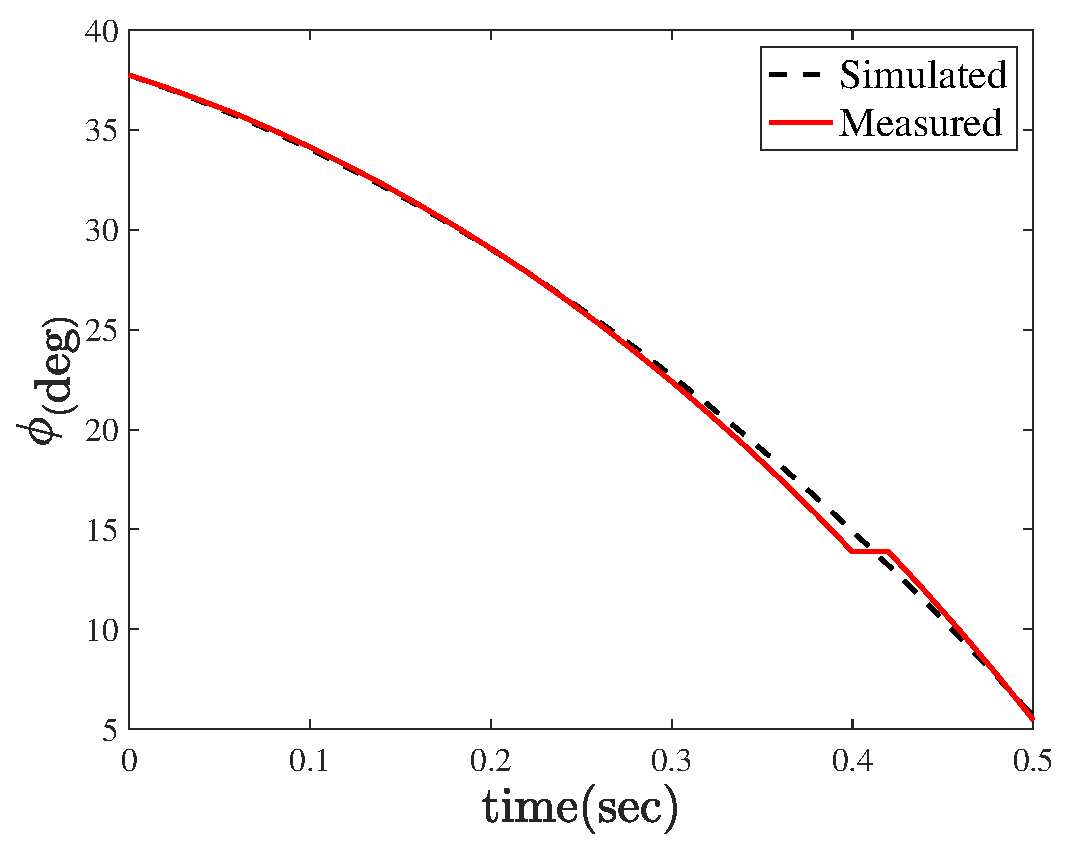
\includegraphics[width=.30\linewidth]{../Figure/parameter_estimation/roll/roll}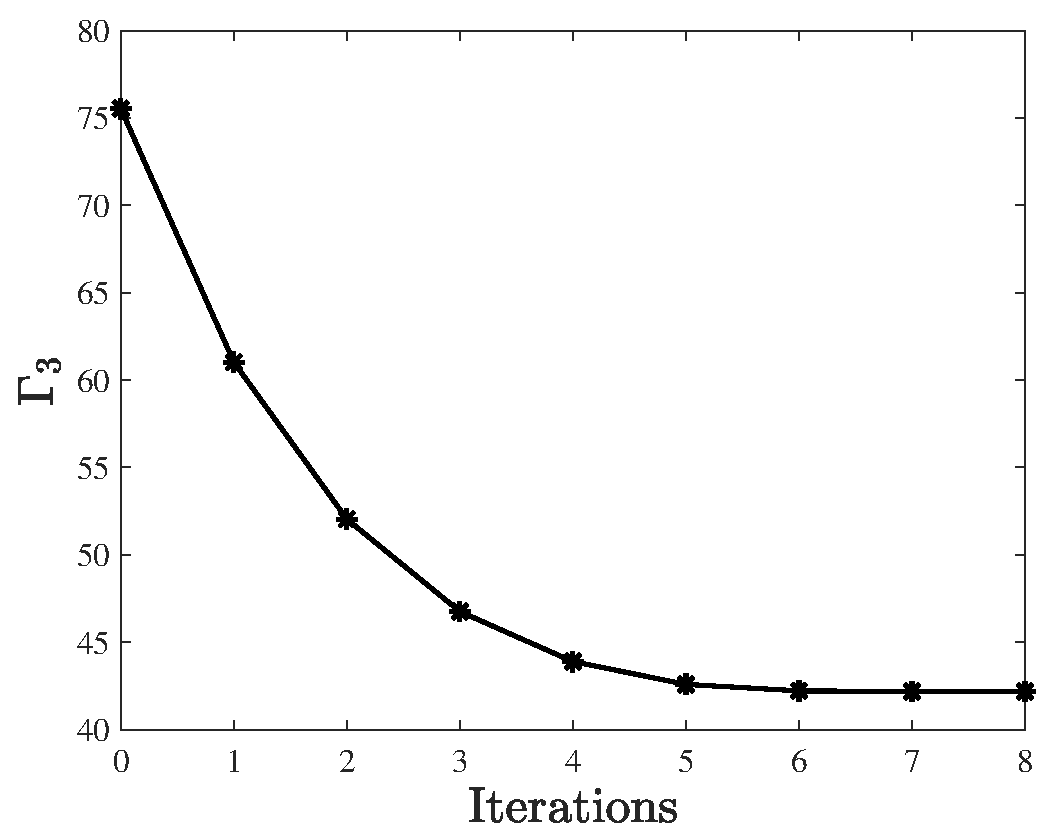
\includegraphics[width=.30\linewidth]{../Figure/parameter_estimation/roll/roll_parameter_Gamma3}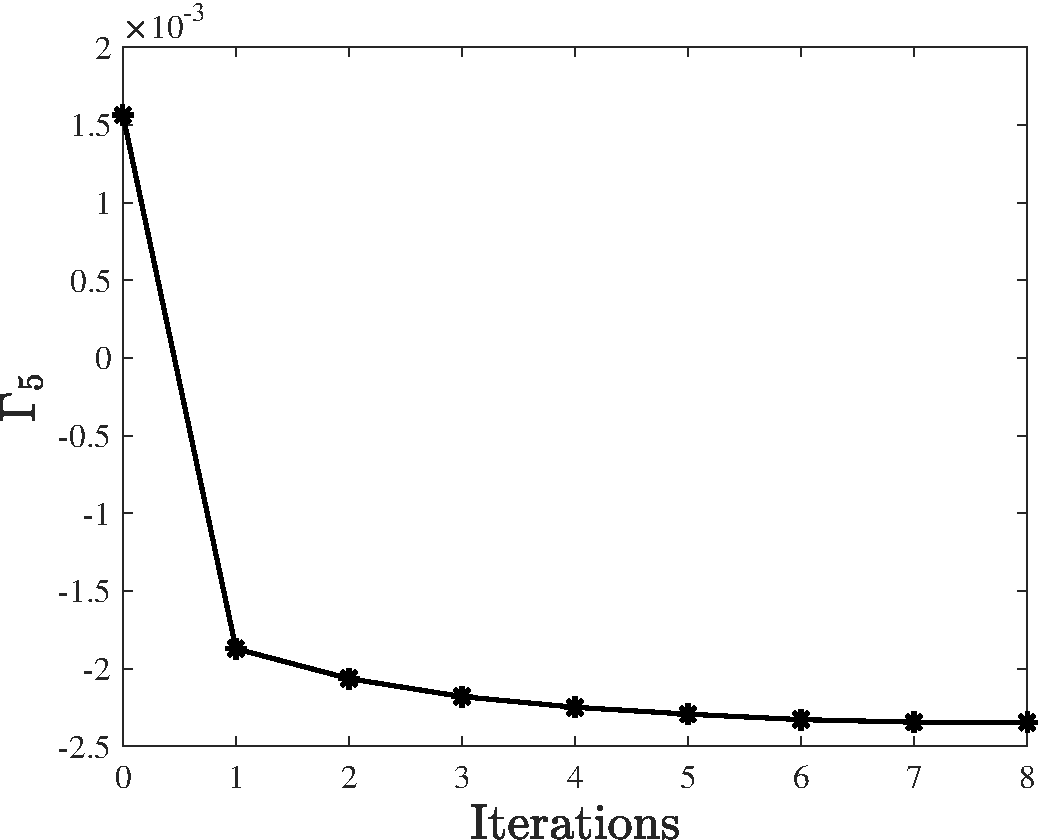
\includegraphics[width=.3\linewidth]{../Figure/parameter_estimation/roll/roll_parameter_Gamma5}
    }
    \hfil
    % \vspace{-0.25cm}
    \subfloat[]{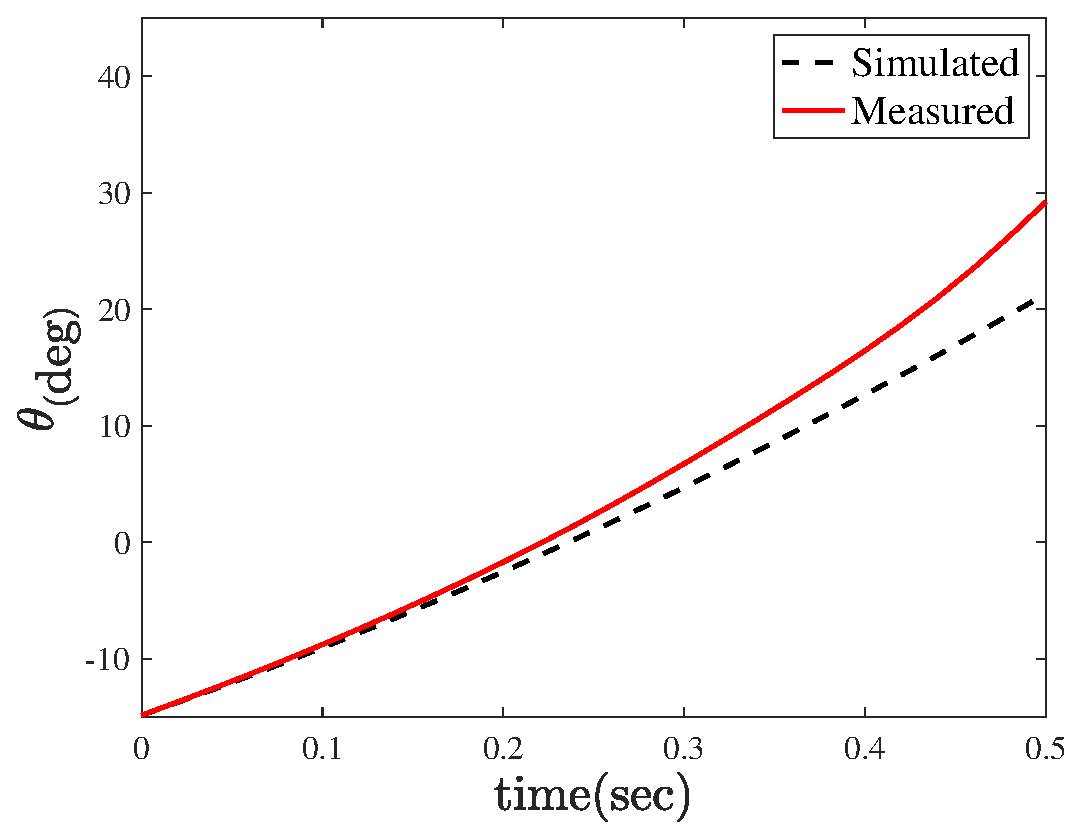
\includegraphics[width=.3\linewidth]{../Figure/parameter_estimation/pitch/pitch}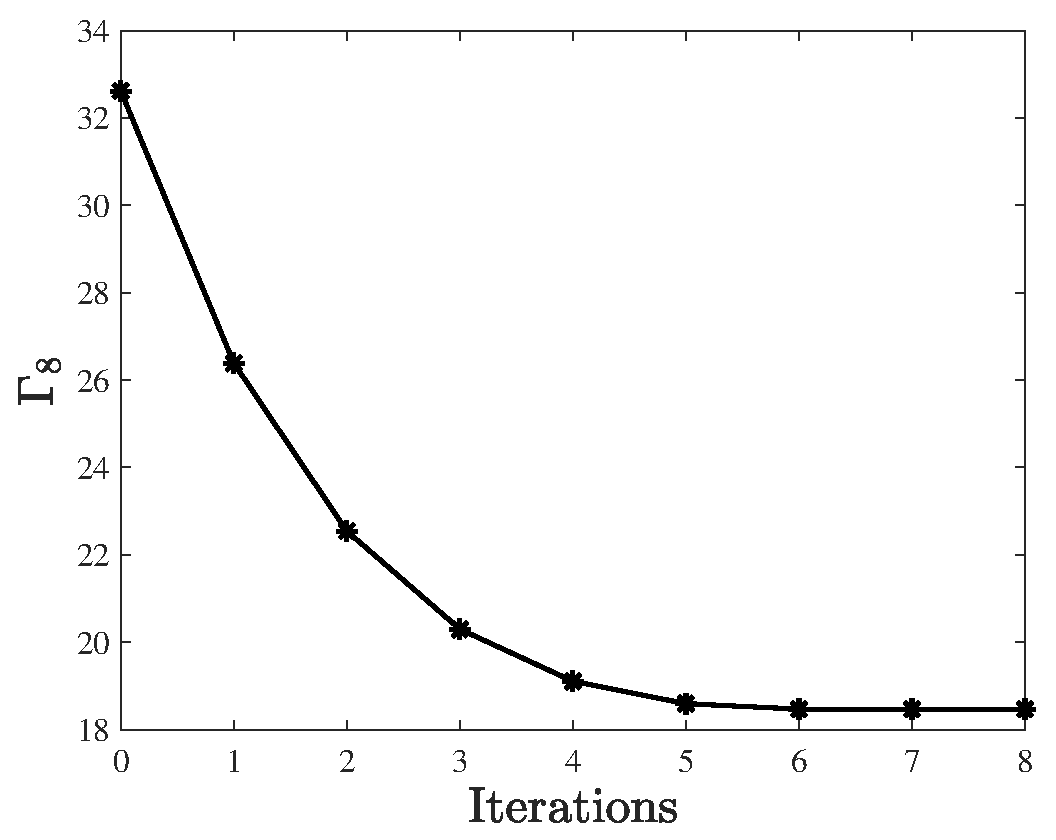
\includegraphics[width=.3\linewidth]{../Figure/parameter_estimation/pitch/pitch_paramete_Gamma8}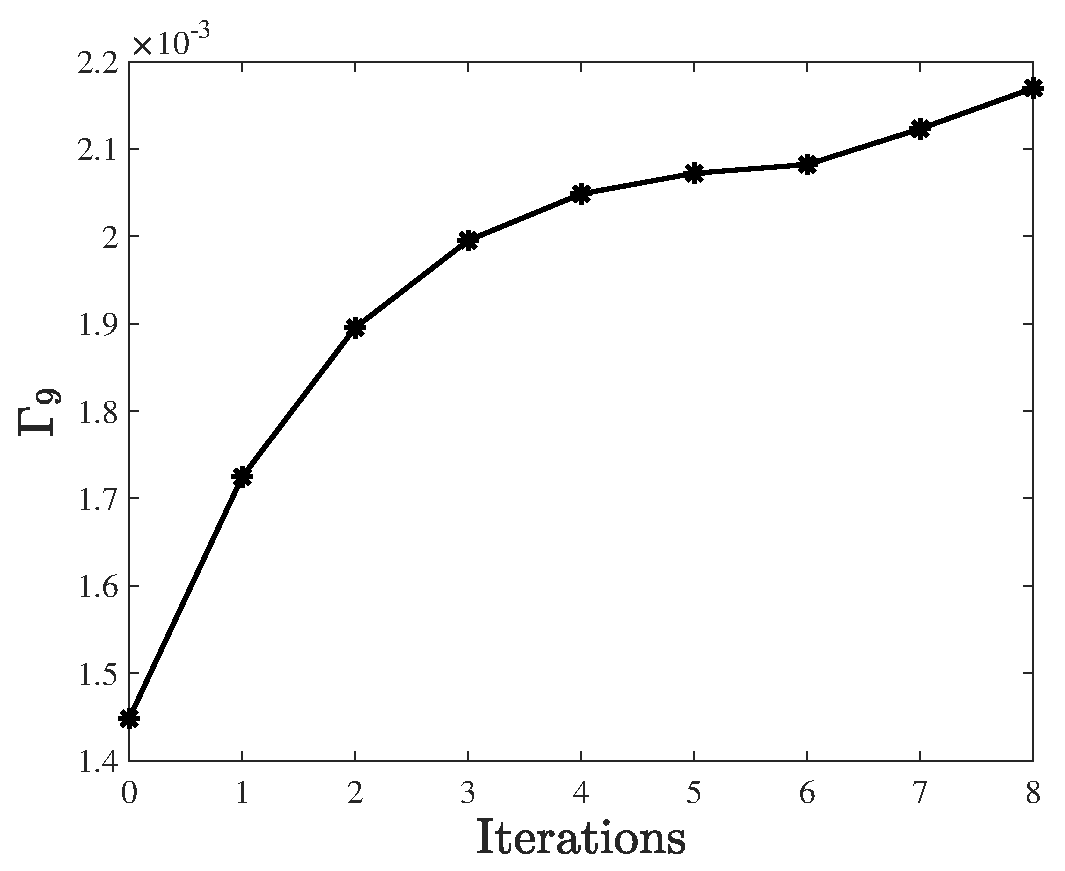
\includegraphics[width=.3\linewidth]{../Figure/parameter_estimation/pitch/pitch_paramete_Gamma9}
    }
    \hfil
    % \vspace{-0.25cm}
    \subfloat[]{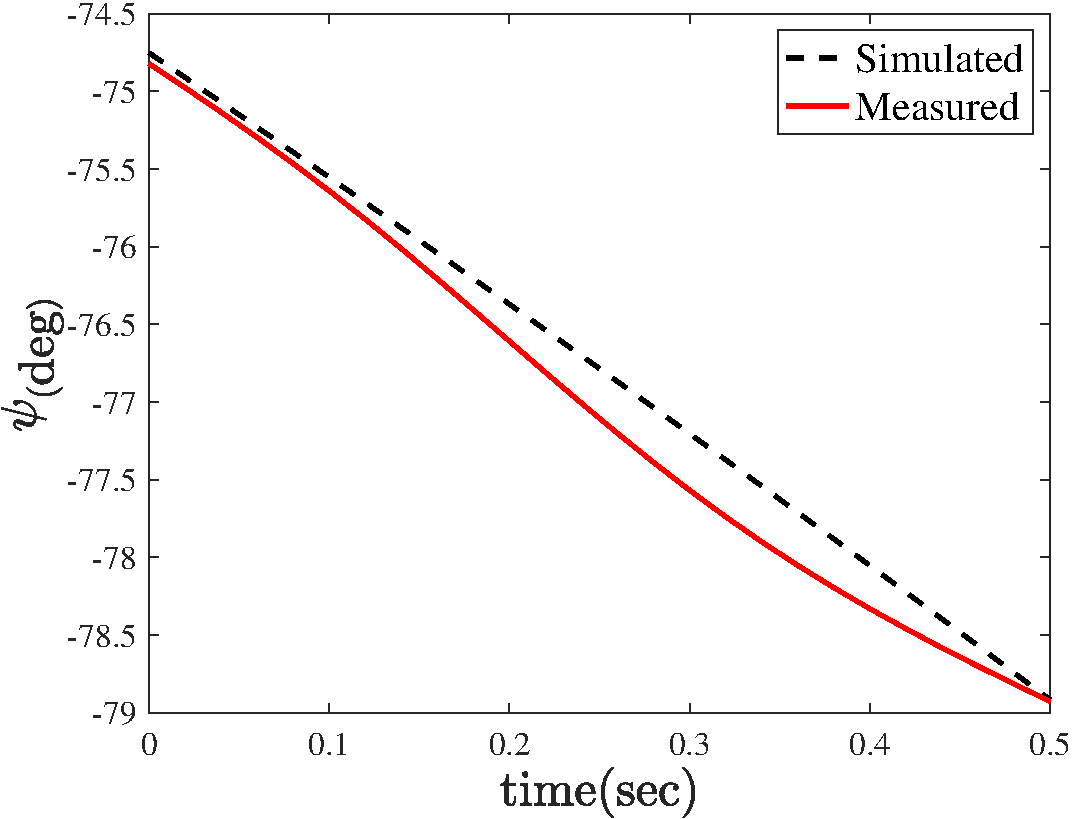
\includegraphics[width=.4\linewidth]{../Figure/parameter_estimation/yaw/yaw}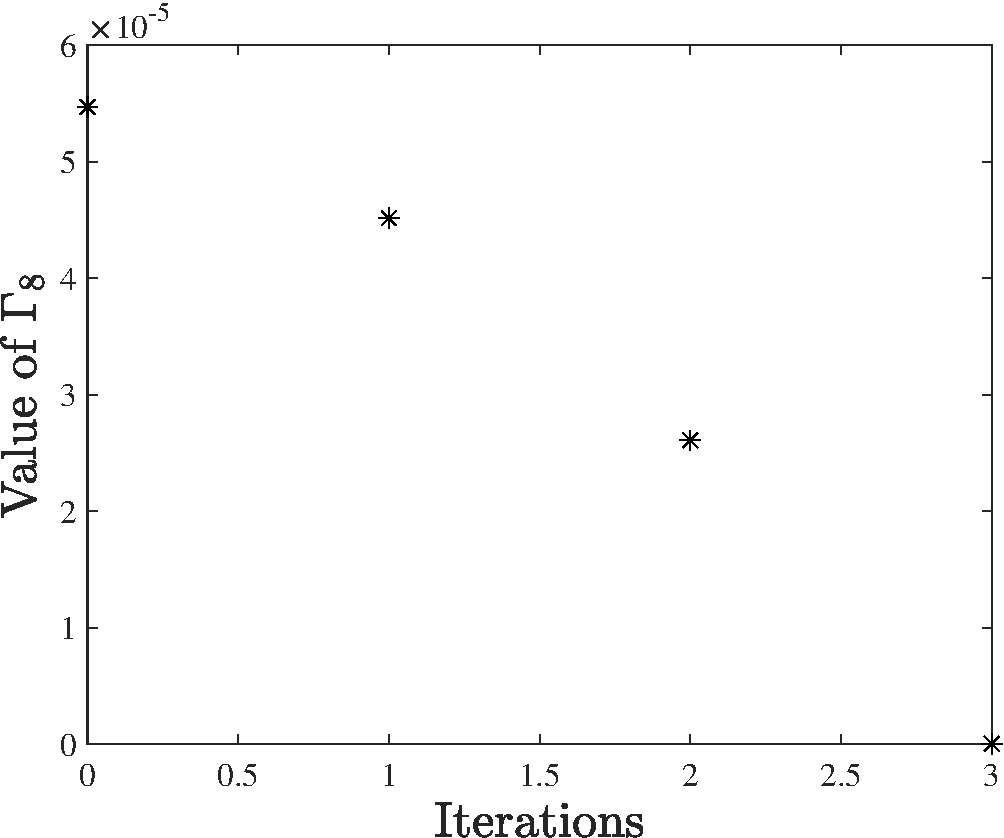
\includegraphics[width=.4\linewidth]{../Figure/parameter_estimation/yaw/yaw_parameter}
    }
    \caption{Identification process results when the quadrotor rotates about only one axis: (a) identification of $\Gamma_3$ and $\Gamma_5$ in free roll motion. (b) identification of $\Gamma_8$ and $\Gamma_9$ in free pitch motion. (c) identification of $\Gamma_{11}$
    in free yaw motion.}
    \label{fig:one_degree_identification}
\end{figure}
\begin{figure}[H]
    \centering
    \vspace{-2.2cm}
    \subfloat[]{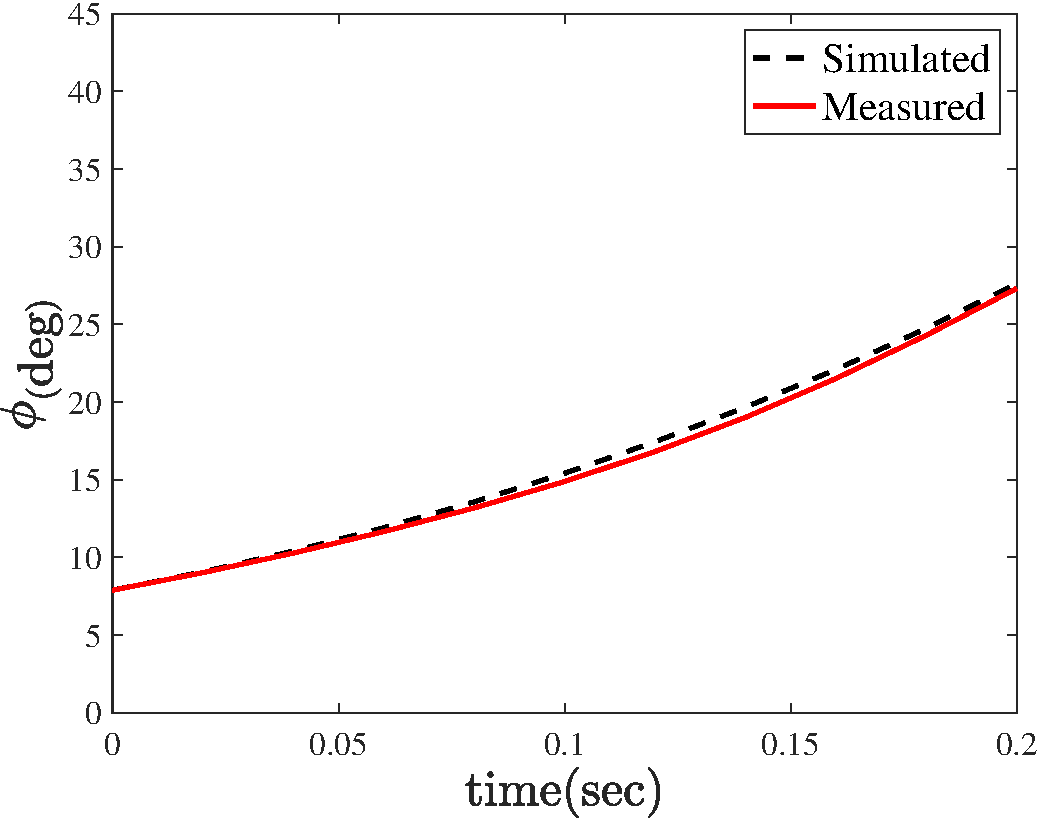
\includegraphics[width=.4\linewidth]{../Figure/parameter_estimation/roll-pitch/roll}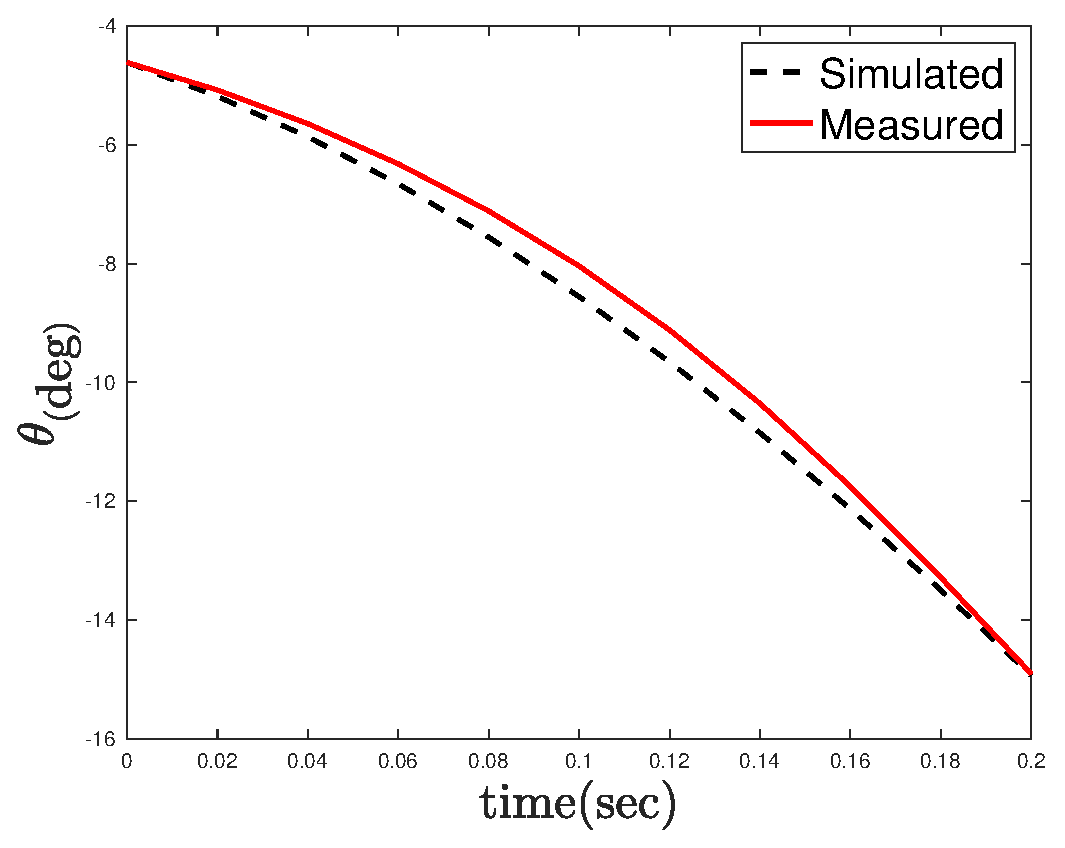
\includegraphics[width=.4\linewidth]{../Figure/parameter_estimation/roll-pitch/pitch}
    }
    \hfil
    % \vspace{-0.25cm}
    \subfloat[]{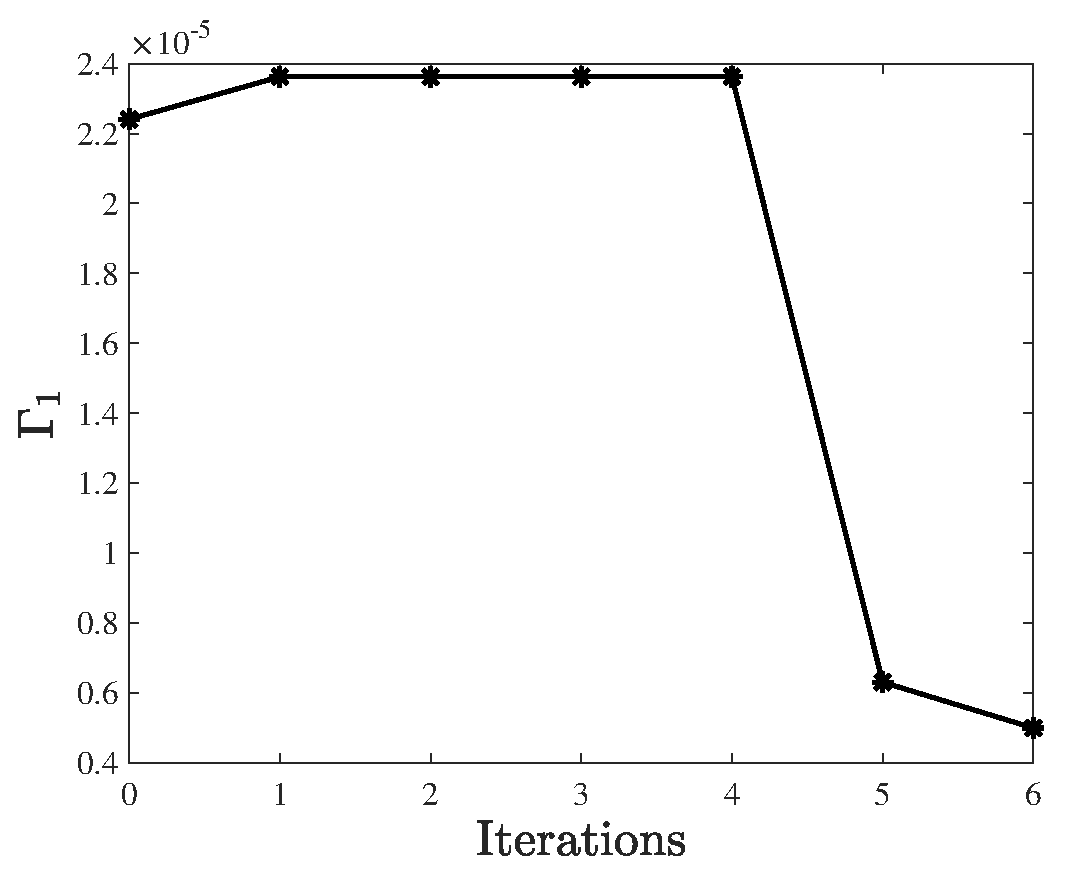
\includegraphics[width=.4\linewidth]{../Figure/parameter_estimation/roll-pitch/pitch_parameter_Gamma1}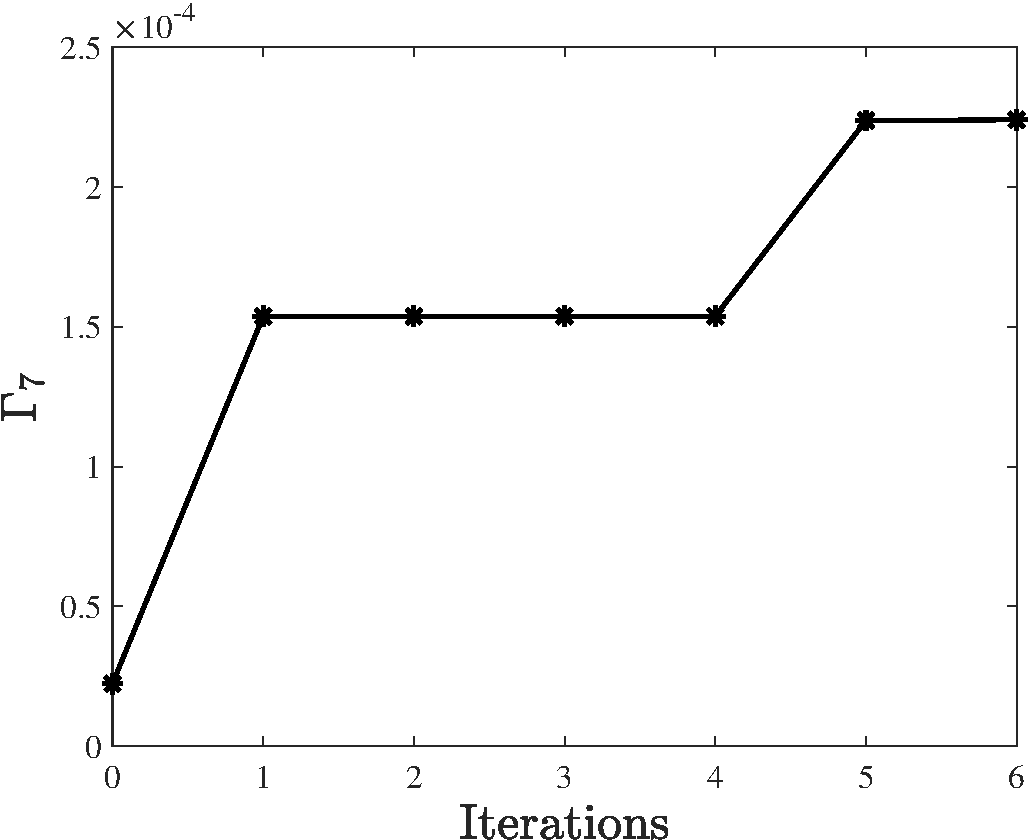
\includegraphics[width=.4\linewidth]{../Figure/parameter_estimation/roll-pitch/pitch_parameter_Gamma7}
    }
    \caption{Identification process results when the quadrotor rotates about its roll and pitch axes:
    (a) comparison of simulation and experimental results. (b) identification of $\Gamma_1$ and $\Gamma_7$.}
    \label{fig:two_degree_identification}
% \end{figure}
% \begin{figure}[H]
    \centering
    \subfloat[]{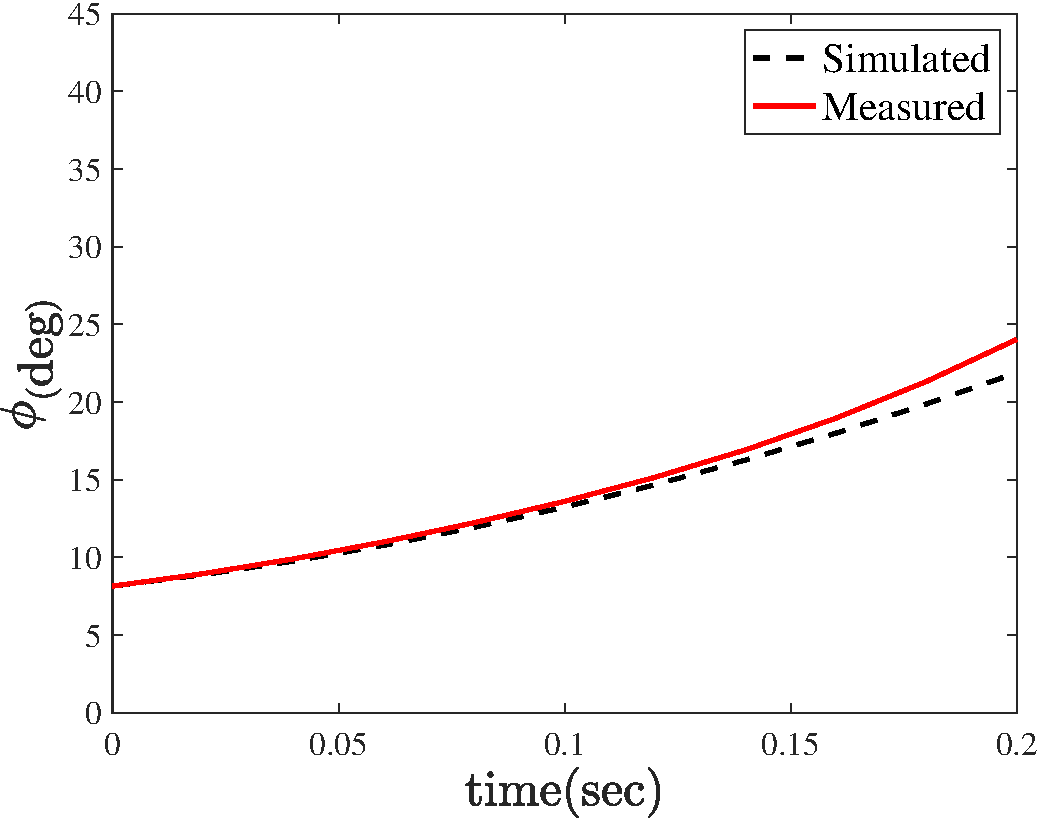
\includegraphics[width=.33\linewidth]{../Figure/parameter_estimation/3DOF/roll}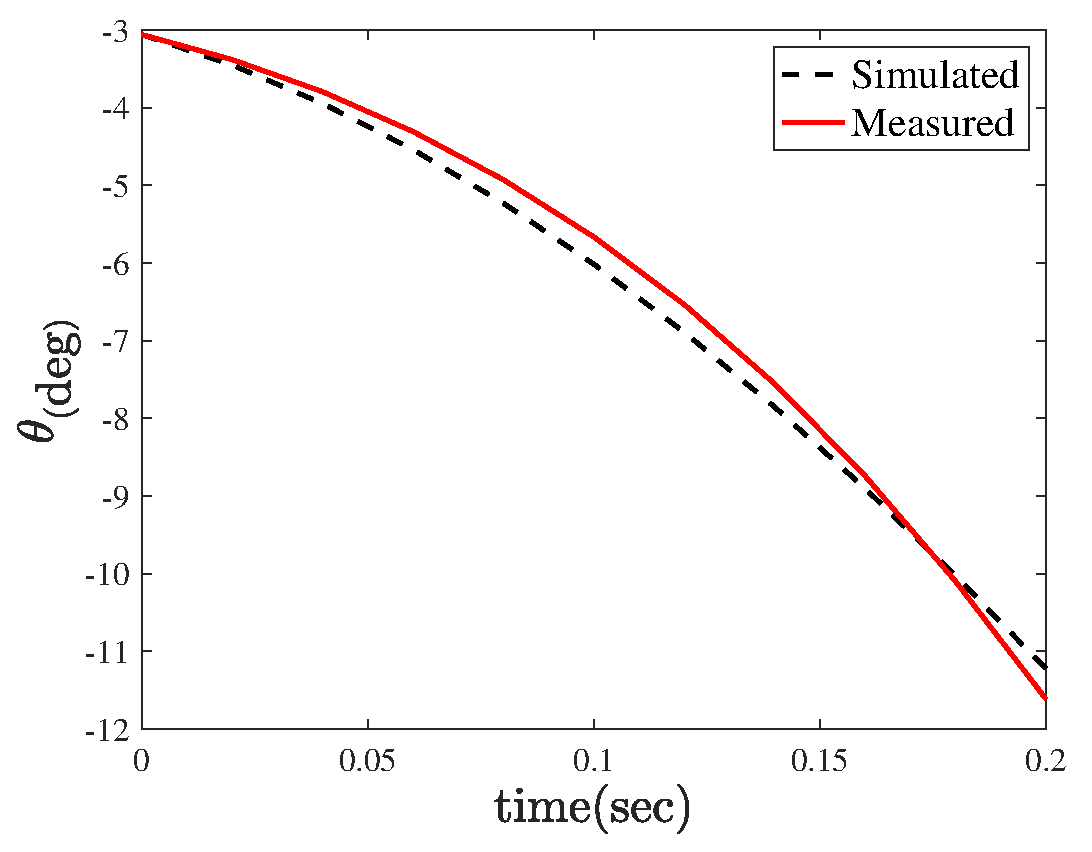
\includegraphics[width=.33\linewidth]{../Figure/parameter_estimation/3DOF/pitch}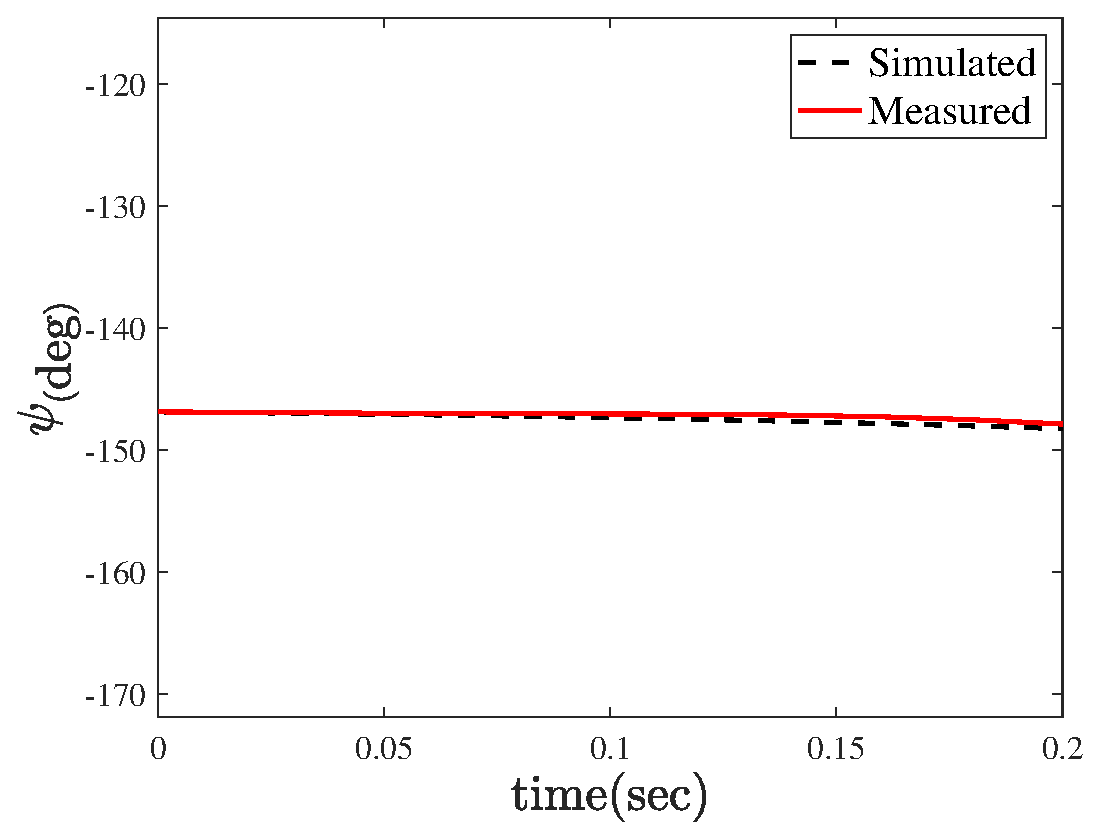
\includegraphics[width=.33\linewidth]{../Figure/parameter_estimation/3DOF/yaw}
    }
    \hfil
    \subfloat[]{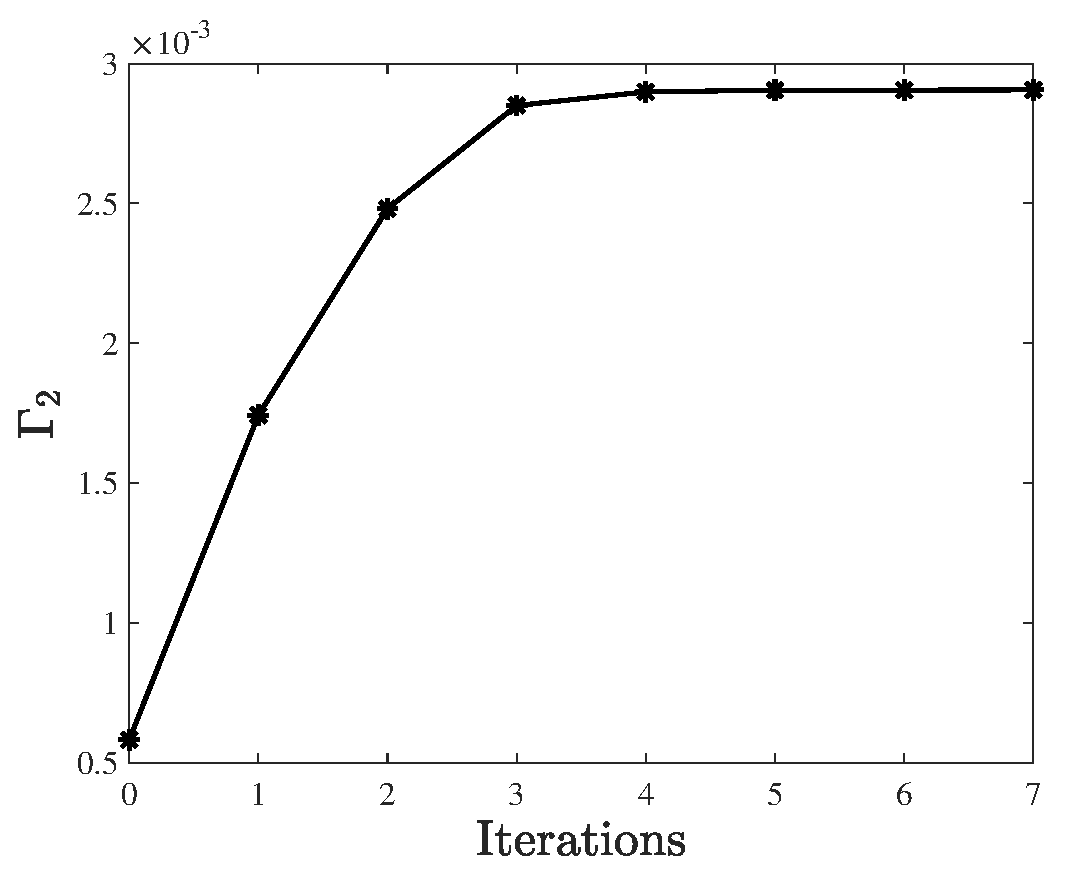
\includegraphics[width=.24\linewidth]{../Figure/parameter_estimation/3DOF/Gamma2}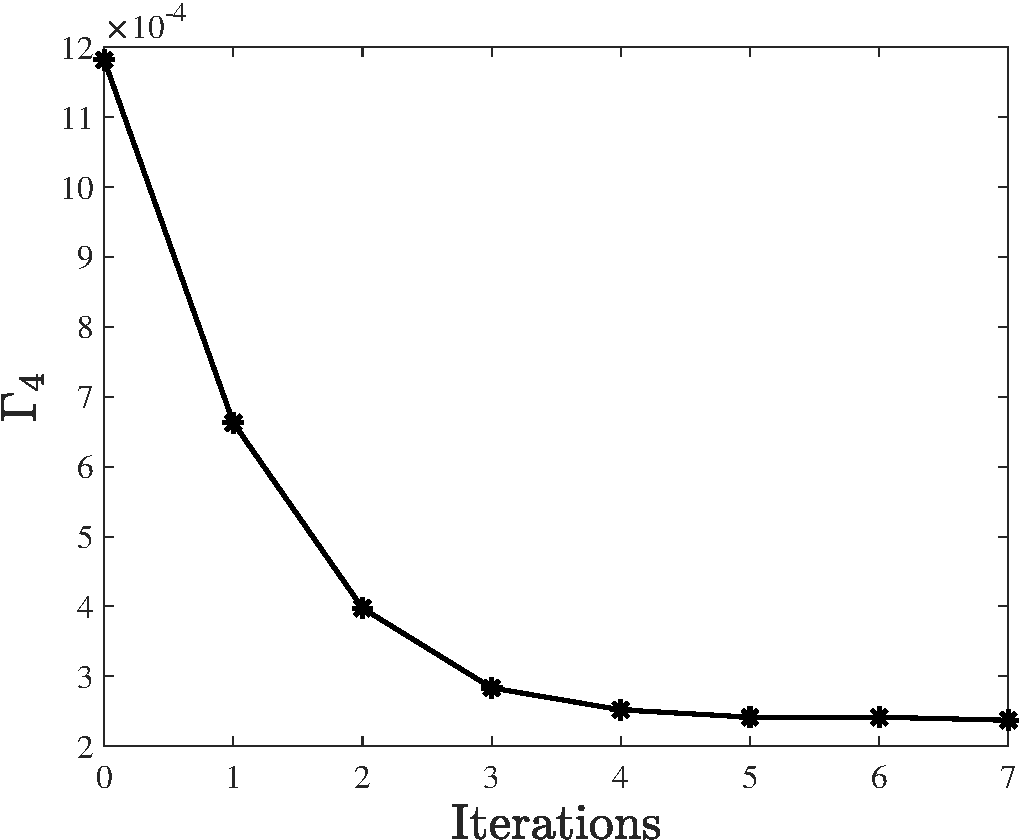
\includegraphics[width=.24\linewidth]{../Figure/parameter_estimation/3DOF/Gamma4}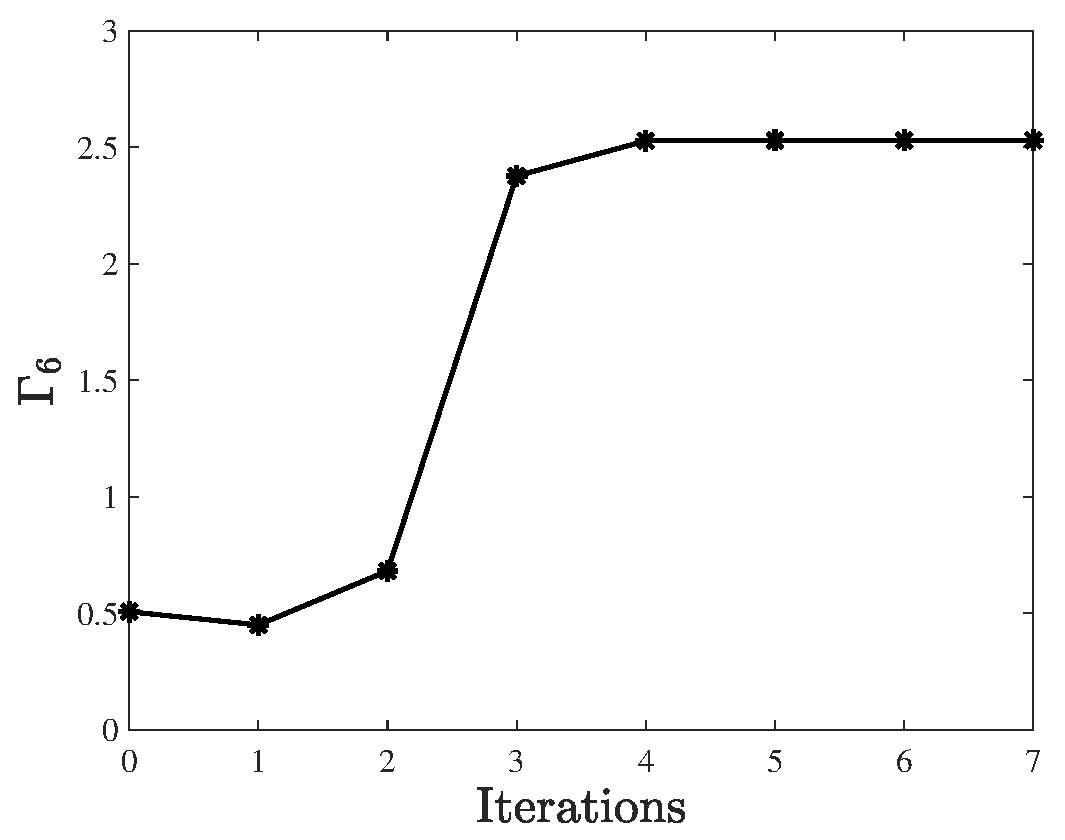
\includegraphics[width=.24\linewidth]{../Figure/parameter_estimation/3DOF/Gamma6}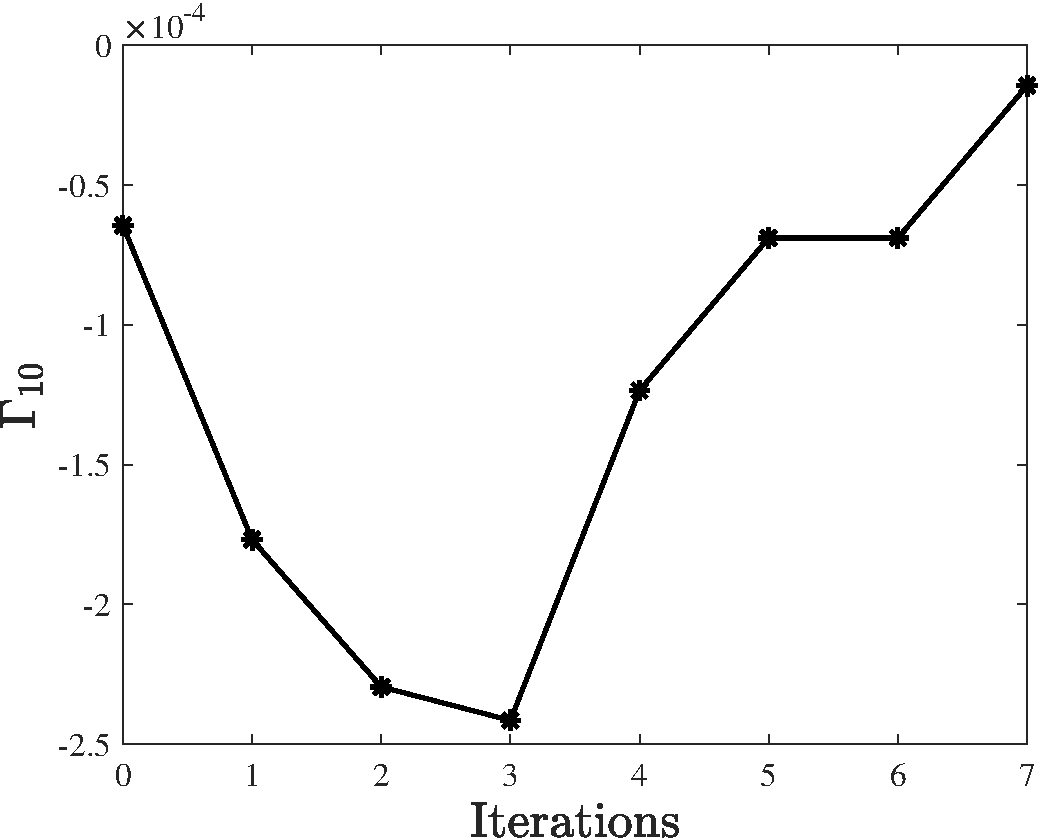
\includegraphics[width=.24\linewidth]{../Figure/parameter_estimation/3DOF/Gamma10}
    }
    \caption{Identification process results when the quadrotor rotates about its roll, pitch, and yaw axes: (a) comparison of simulation and experimental results. (b) identification of $\Gamma_2$, $\Gamma_4$, $\Gamma_6$, and
    $\Gamma_{10}$ parameters.}
    \label{fig:three_degree_identification}
\end{figure}
\subsection{Evaluation of LQIR-DG Performance}
\noindent In this section, the LQIR-DG controller algorithm is evaluated in three scenarios i) regulation and tracking problems, ii) disturbance rejection, and iii) impact of model uncertainty.
Finally, a comparison of the proposed controller is performed with a PID controller and variants of the LQR controller. 
The PID controller parameters are presented in Table~\ref{tab:PID_parameters}.
\begin{table}[H]
    \renewcommand{\arraystretch}{1.3}
    \caption{PID controller parameters}
    \vspace{-0.5cm}
    \begin{center}
        \begin{tabular}{cccc}
        \hline
        \textbf{Channel} & \textbf{$K_p$} & \textbf{$K_i$} & \textbf{$K_d$} \\
        \hline
        roll & 18 & 6 & 9 \\
        pitch & 22 & 15 & 16 \\
        \hline
        \end{tabular}
        \label{tab:PID_parameters}
    \end{center}
\end{table}
\subsubsection{Investigating of the Regulation and Tracking Problems}\label{sec:regulation}
\noindent The results of the proposed approach are presented for tracking the desired roll and pitch angles in Figures~\ref{fig:result} and~\ref{fig:omega}.
 %%%? so many of
Figure~\ref{fig:result}~\ref{sub@fig:regulation} compares the desired and output signals, i.e., the Euler angles during the regulation problem. Moreover, Figure~\ref{fig:result}~\ref{sub@fig:square} compares the desired square wave signals with a frequency of 0.02 Hz and an amplitude of 20 degrees with the output signals, when the quadrotor platform freely rotates around roll and pitch, simultaneity.
Figures~\ref{fig:omega}~\ref{sub@fig:omega_regulation} and~\ref{sub@fig:omega_square} show the rotational velocity commands of the quadrotor in the regulation and tracking problems, respectively. These results demonstrate that the roll and pitch angles are accurately controlled by the proposed approach.


\begin{figure}[H]
    \centering
    \vspace{0.3cm}
    \subfloat[\label{fig:regulation}]{{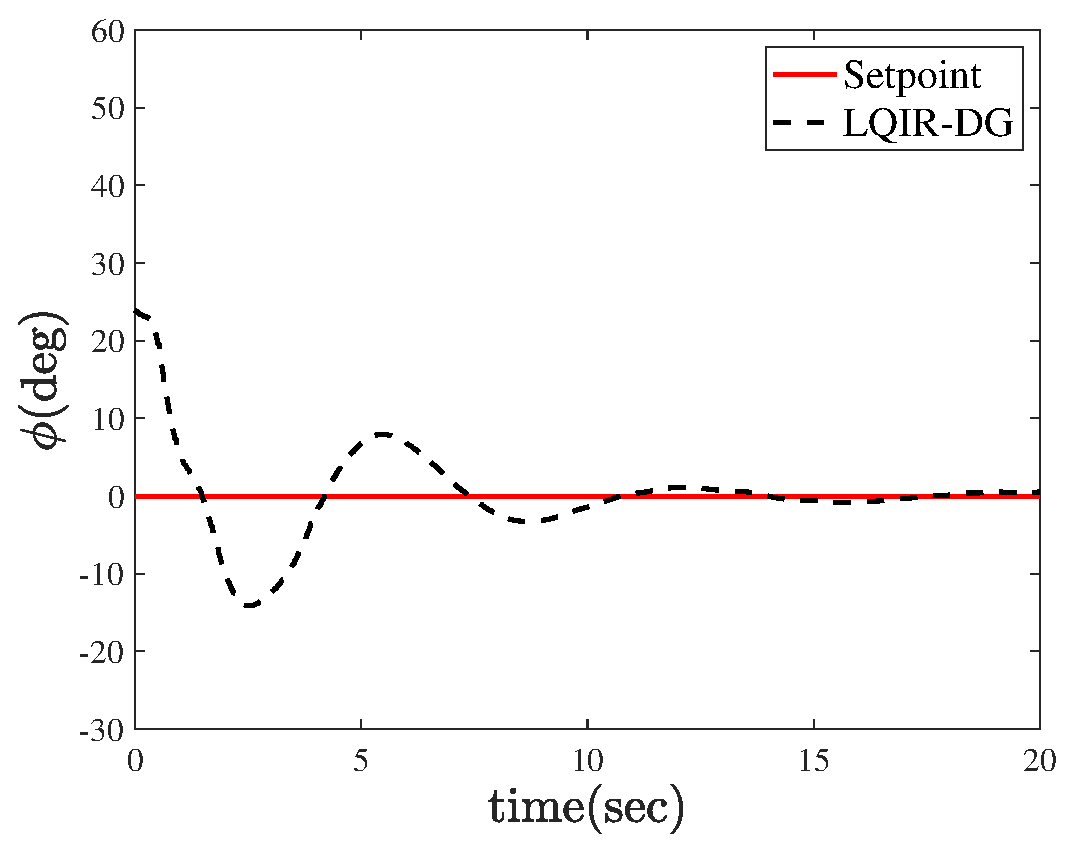
\includegraphics[width=.33\linewidth]{../Figure/implementation/lqidg_roll}}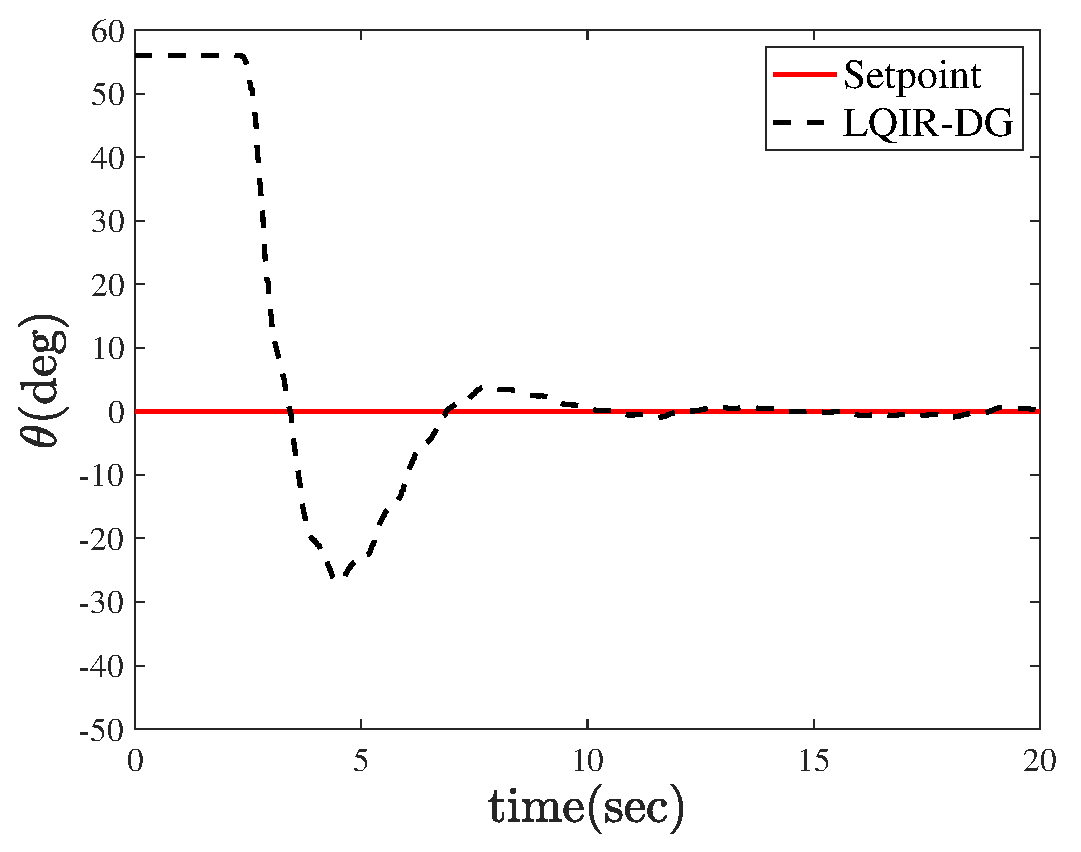
\includegraphics[width=.33\linewidth]{../Figure/implementation/lqidg_pitch}
    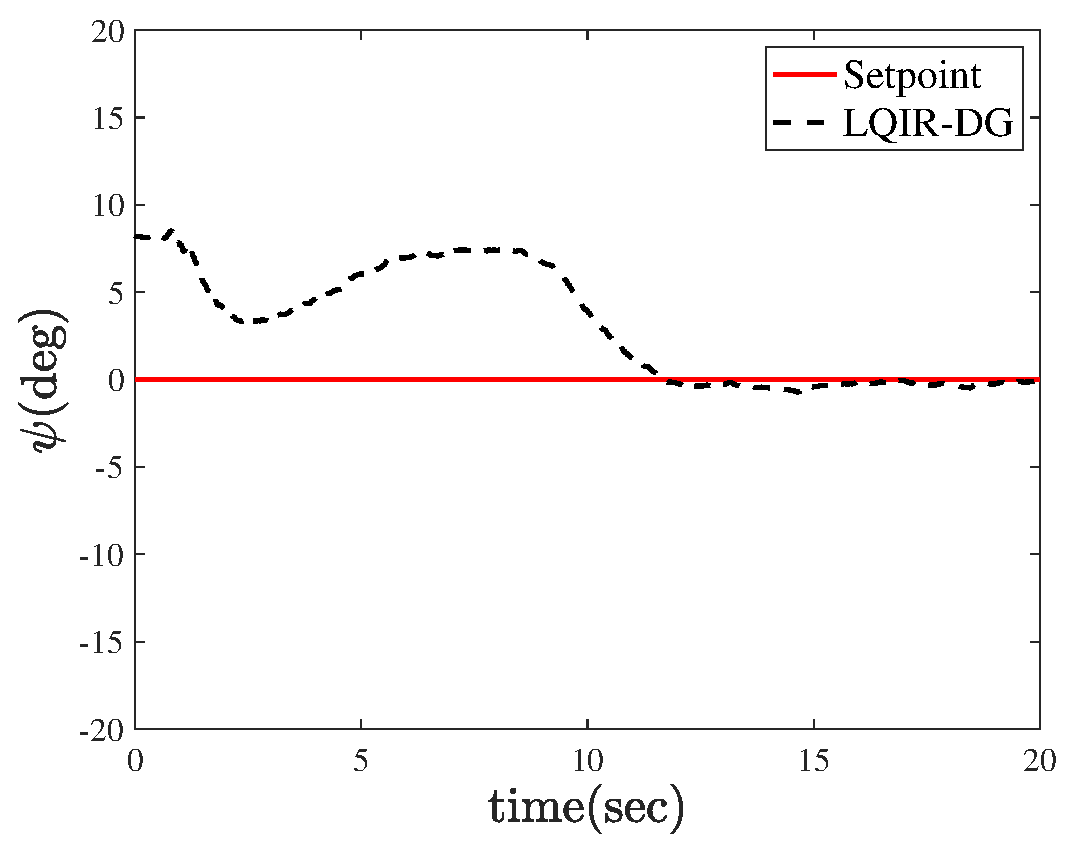
\includegraphics[width=.33\linewidth]{../Figure/implementation/lqidg_yaw}}
    \hfill
    \subfloat[\label{fig:square}]{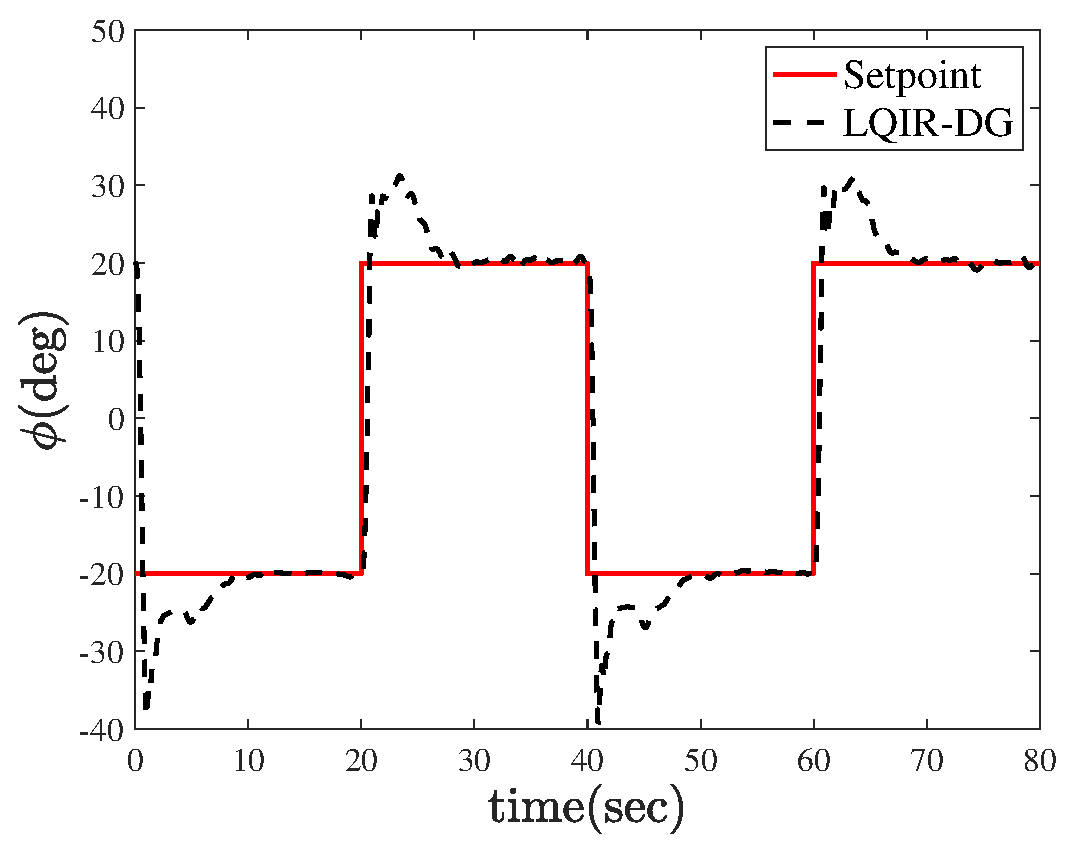
\includegraphics[width=.35\linewidth]{../Figure/implementation/square/lqidg_roll_20}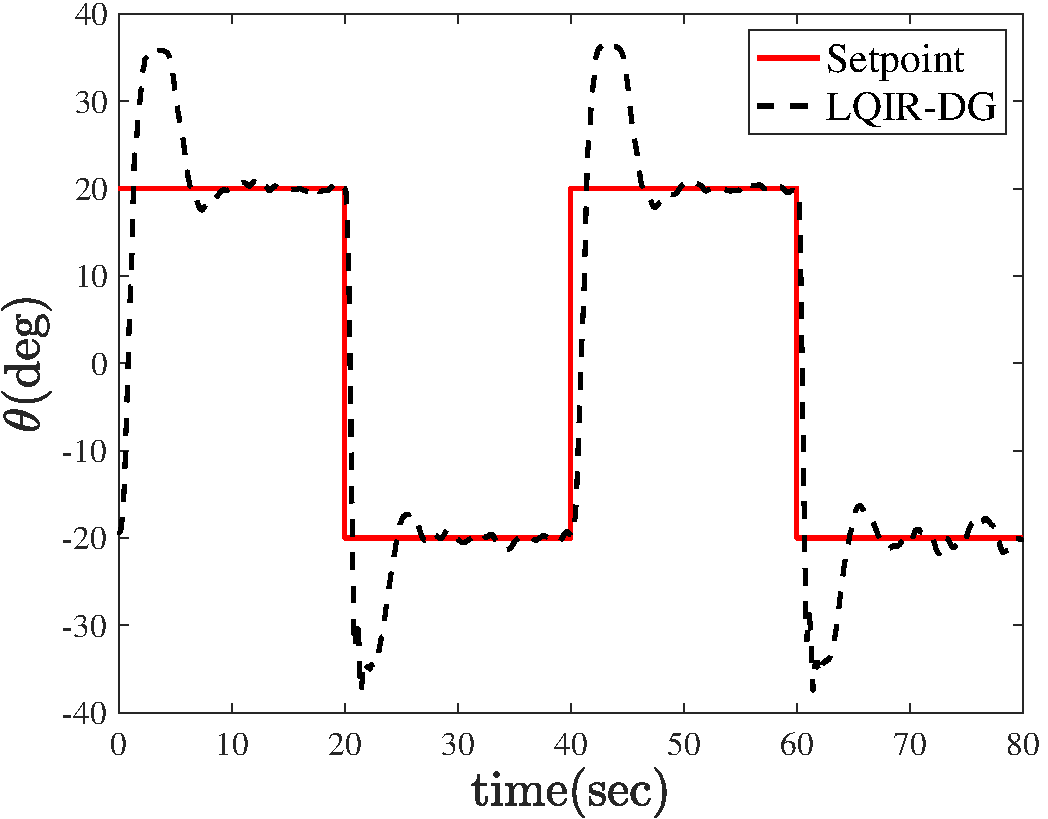
\includegraphics[width=.35\linewidth]{../Figure/implementation/square/lqidg_pitch_20}}
    \caption{Comparison of actual roll and pitch angles with the desired values in~\ref{sub@fig:regulation} regulation and~\ref{sub@fig:square} tracking problems.}
    \label{fig:result}
\end{figure}

\begin{figure}[H]
    \vspace{0.3cm}
    \centering
    \subfloat[\label{fig:omega_regulation}]{\includegraphics[width=.25\linewidth]{../Figure/implementation/lqidg_Omega_1}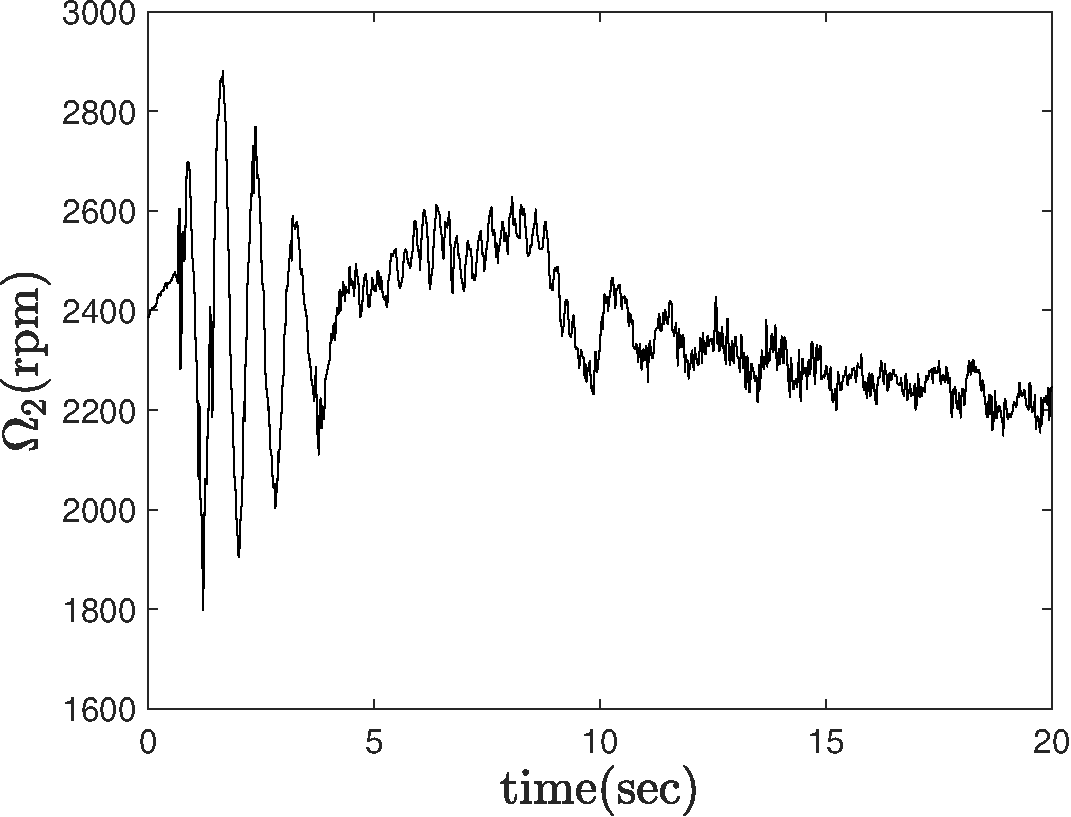
\includegraphics[width=.25\linewidth]{../Figure/implementation/lqidg_Omega_2}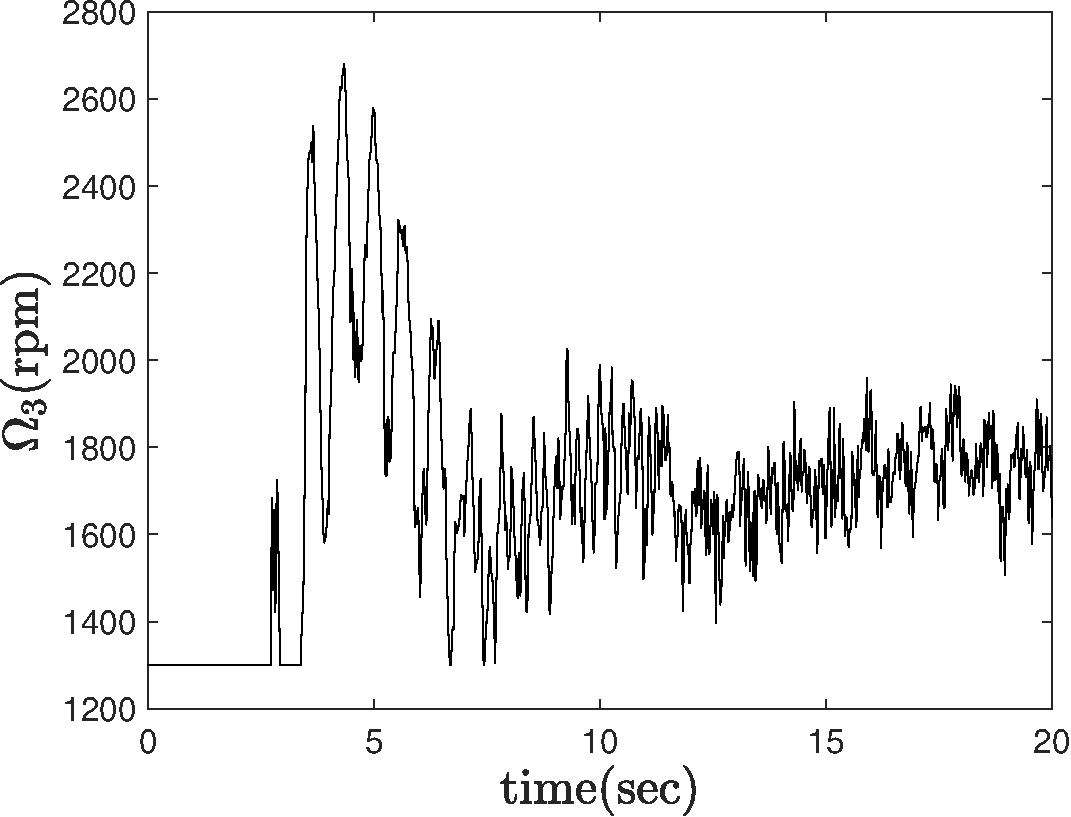
\includegraphics[width=.25\linewidth]{../Figure/implementation/lqidg_Omega_3}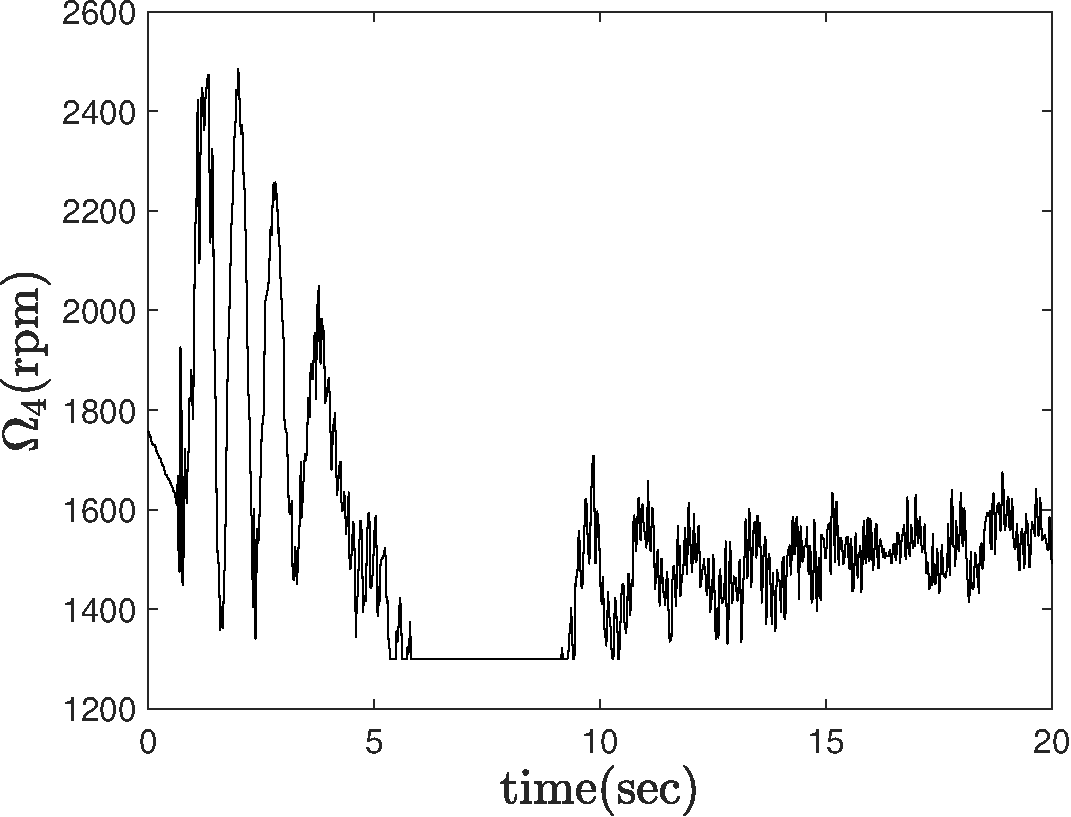
\includegraphics[width=.25\linewidth]{../Figure/implementation/lqidg_Omega_4}
    }
    \hfil
    \subfloat[\label{fig:omega_square}]{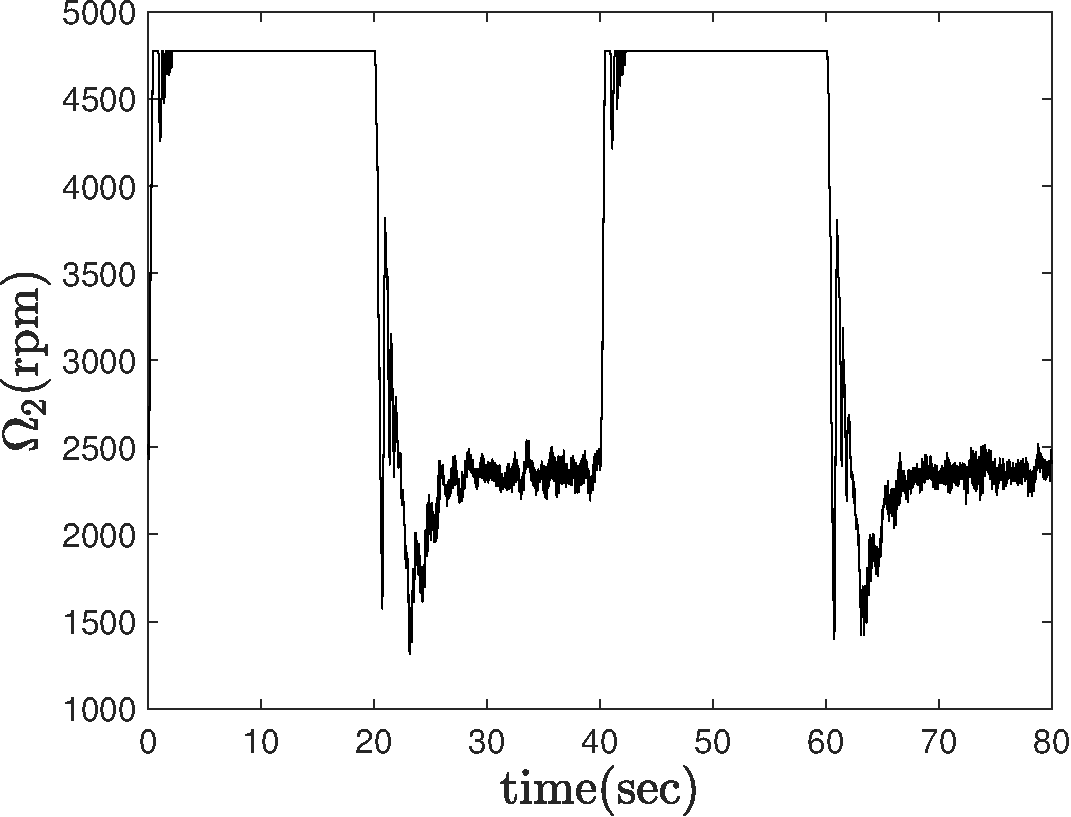
\includegraphics[width=.25\linewidth]{../Figure/implementation/square/lqidg_squre_omega_2}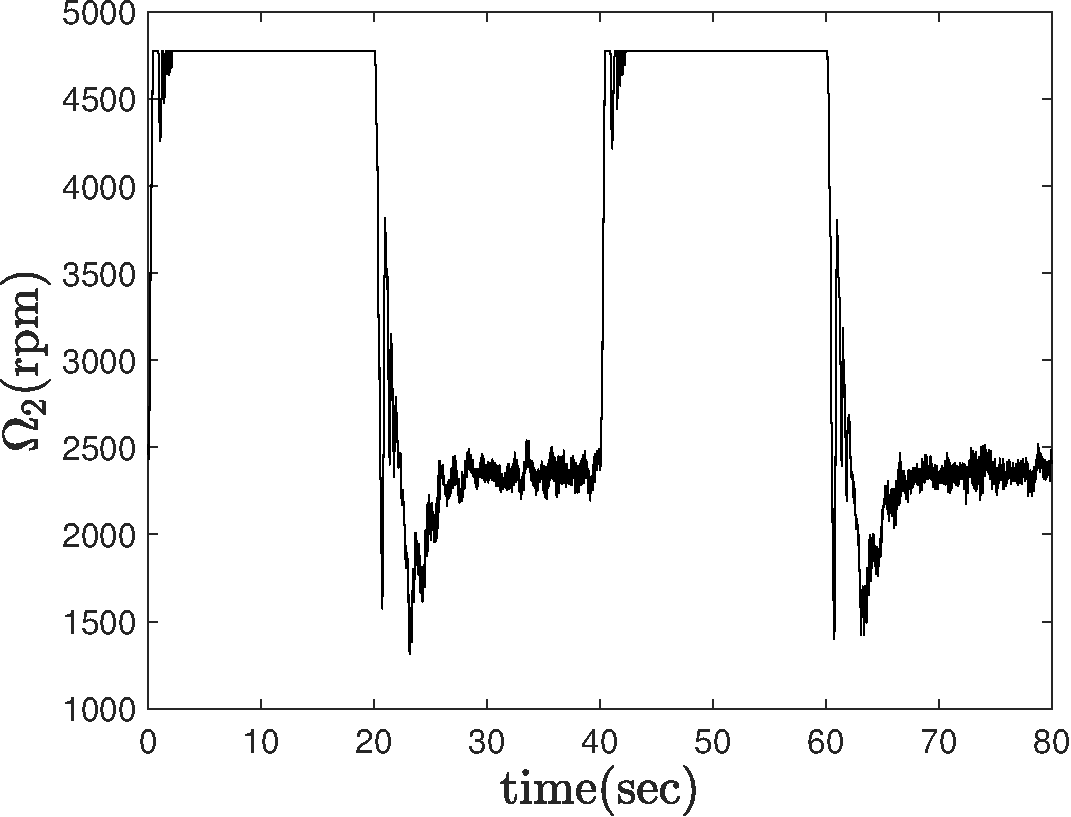
\includegraphics[width=.25\linewidth]{../Figure/implementation/square/lqidg_squre_omega_2}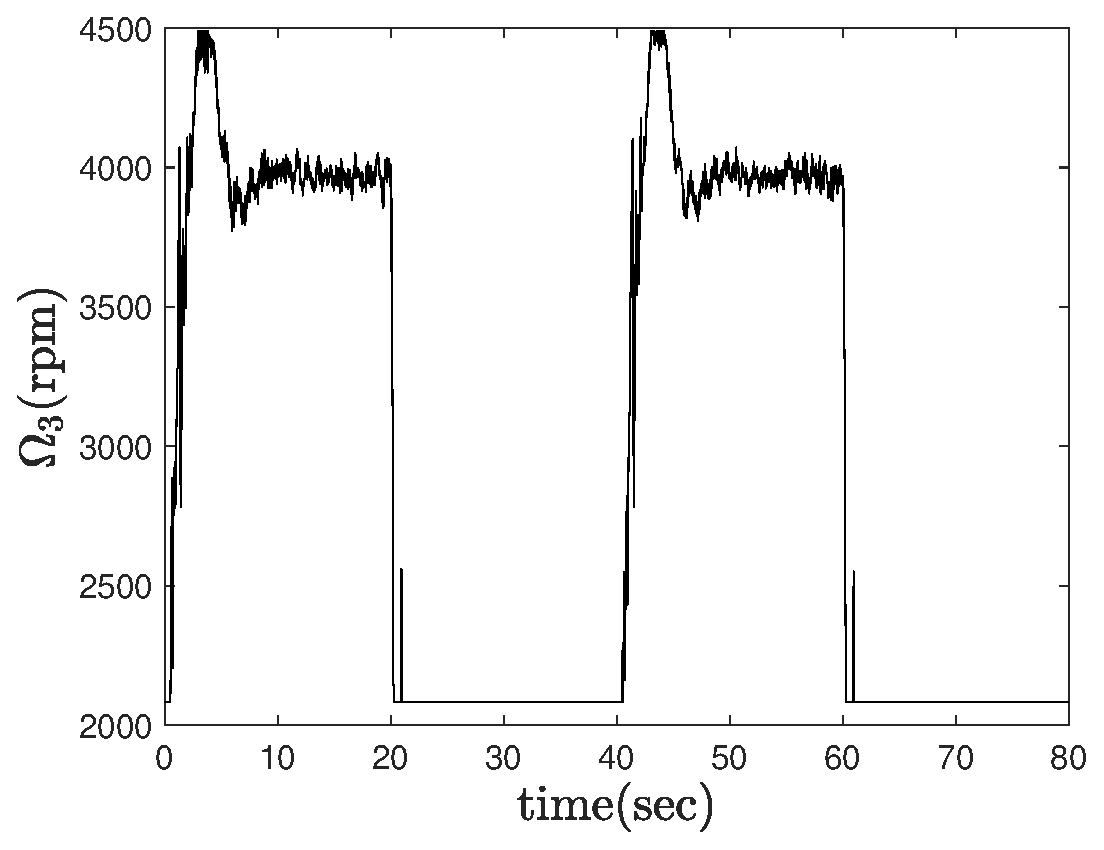
\includegraphics[width=.25\linewidth]{../Figure/implementation/square/lqidg_squre_omega_3}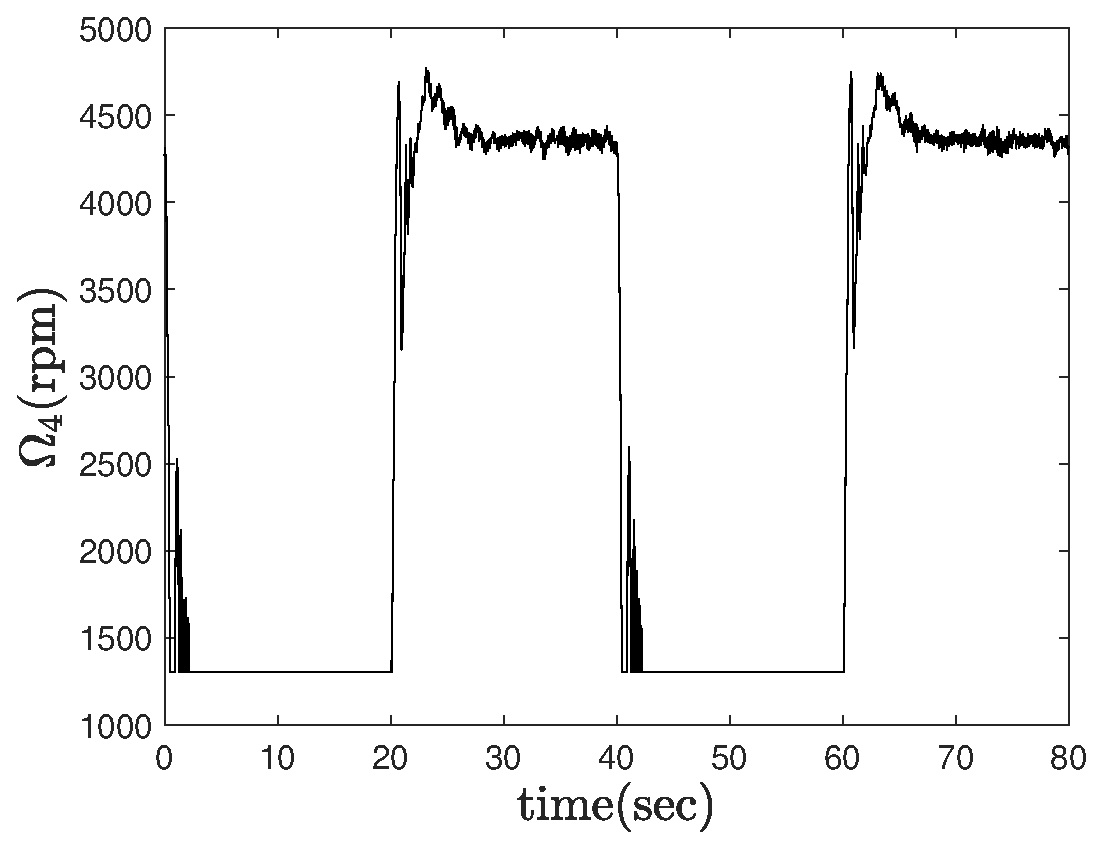
\includegraphics[width=.25\linewidth]{../Figure/implementation/square/lqidg_squre_omega_4}} %%%? didnt describe a and b
    \caption{Rotational velocity  commands in~\ref{sub@fig:omega_regulation} regulation and~\ref{sub@fig:omega_square} tracking problems.}
    \label{fig:omega}
\end{figure}
\subsubsection{Investigating the Disturbance Rejection}\label{sec:disturbance}
\noindent Here, the effect of the input disturbance is investigated on the performance of the proposed controller.
The input disturbance, $\mathrm{d_{\Omega_i}}$, is considered as a change in command of the rotational velocity, modeled as %%%? with or in for input disturbance

\begin{equation}
    \mathrm{d_{\Omega_1}} = \mathrm{d_{\Omega_2}} = -\mathrm{d_{\Omega_3}} = -\mathrm{d_{\Omega_4}} = \begin{cases}
        500~{\mathrm{rpm}} \quad &20<t<60\\
        0 \quad &\mathrm{otherwise}
    \end{cases}
    \label{eq:disturbance}
\end{equation}

Figure~\ref{fig:disturbance} illustrates the roll and pitch angles in the regulation problem when the input disturbance occurs. These results indicate that the proposed controller can stabilize the quadrotor platform in the presence of input disturbance.

% Additionally, a comparative analysis is conducted to evaluate the performance of the proposed Linear Quadratic Integral Differential Game (LQIR-DG) controller against two other well-known disturbance rejection methods: Active Disturbance Rejection Control (ADRC) and Disturbance Observer-Based Control (DOBC).

% \textbf{Active Disturbance Rejection Control (ADRC):}
% (ADRC) is a robust control method widely used to handle uncertainties and disturbances in dynamic systems. It relies on the concept of an extended state observer to estimate and compensate for disturbances, allowing for improved control performance. ADRC has gained popularity in various fields due to its ability to deal with disturbances in real-time and enhance system robustness.

% In ADRC, an extended state observer estimates the total disturbances affecting the system, including external disturbances and model uncertainties. By actively rejecting these disturbances, ADRC ensures accurate tracking and control of the system. The control law in ADRC is designed to incorporate the estimated disturbances and adjust the control inputs accordingly to minimize the effects of disturbances on the system.

% One of the key advantages of ADRC is its simplicity and ease of implementation, making it suitable for a wide range of control applications. The ability to handle uncertainties and disturbances in real-time allows ADRC to achieve better performance and stability compared to traditional control methods in challenging and dynamic environments.

% \textbf{Disturbance Observer-Based Control (DOBC):}
% (DOBC) is robust control strategy used to estimate and compensate for external disturbances affecting the system. DOBC employs a disturbance observer to accurately estimate the disturbances and uses this information to modify the control inputs accordingly.

% DOBC is designed to address disturbances that cannot be directly measured but can significantly affect the system's behavior. By accurately estimating and compensating for these disturbances, DOBC improves the system's tracking and control performance, especially in the presence of uncertainties and external perturbations.

% The implementation of DOBC involves designing an observer that accurately estimates the disturbances based on the system's dynamics and available measurements. The observer continuously updates its estimates, allowing the controller to adapt and respond to changing disturbance conditions.

% Both ADRC and DOBC are effective tools for disturbance rejection and robust control in dynamic systems. Their ability to estimate and compensate for disturbances contributes to improved system stability and tracking performance, making them valuable options for various control applications, including quadrotor platforms.

% Figure~\ref{fig:disturbance} illustrates the roll and pitch angles during the regulation problem when the input disturbance occurs. The results demonstrate the superior disturbance rejection capabilities of the proposed LQIR-DG controller compared to ADRC and DOBC. The LQIR-DG approach exhibits robust stabilization and superior tracking performance in the presence of input disturbances, further validating the effectiveness of our proposed method.

% Overall, the comparative analysis highlights the remarkable disturbance rejection capabilities of the LQIR-DG controller, positioning it as a promising and impactful choice for controlling quadrotor platforms in real-world scenarios.

\begin{figure}[H]
    \centering
    \subfloat{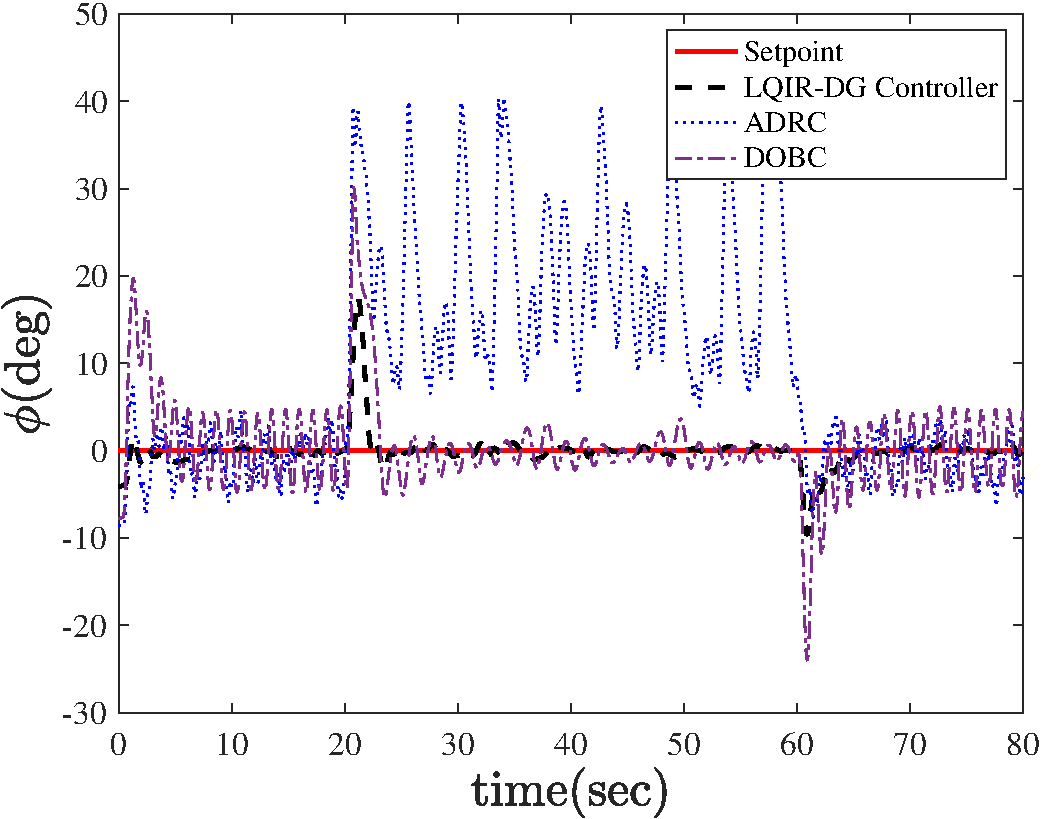
\includegraphics[width=.49\linewidth]{../Figure/implementation/disturbance/lqidg_dis_compare_roll}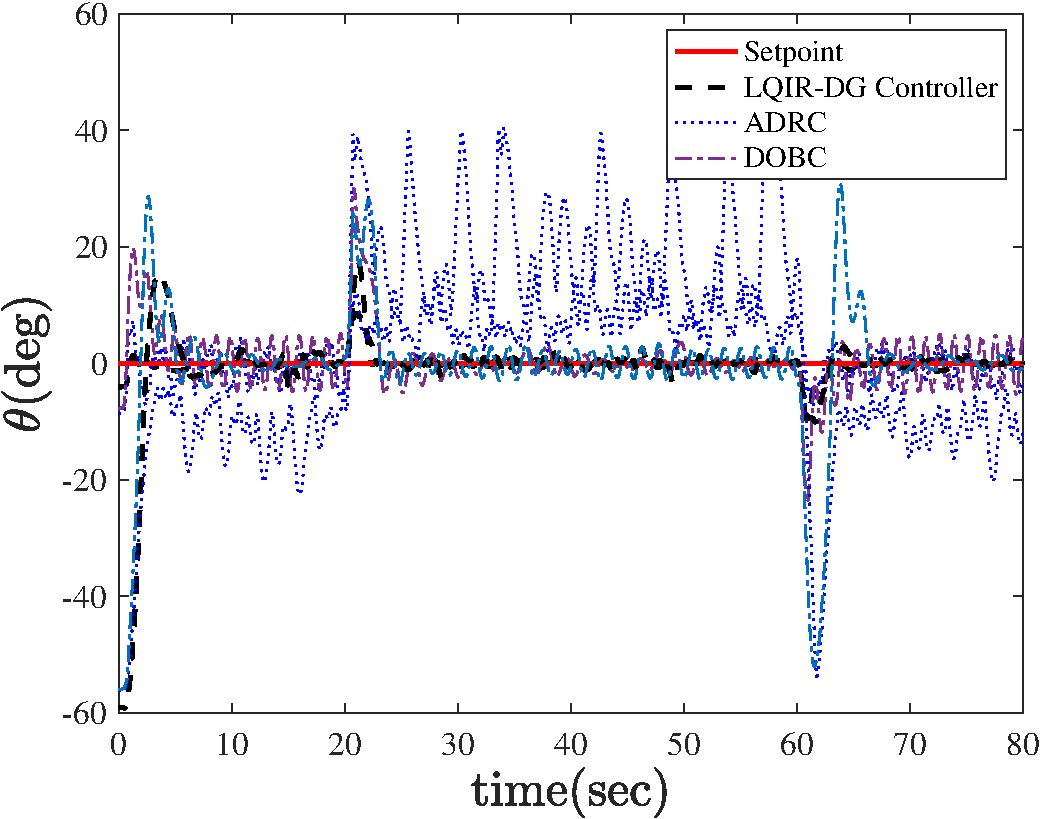
\includegraphics[width=.49\linewidth]{../Figure/implementation/disturbance/lqidg_dis_compare_pitch}
    }
    
    \caption{Comparison of actual roll and pitch angles with the desired, when the input disturbance occurs.}
    \label{fig:disturbance}
\end{figure}
\subsubsection{Investigating the Impact of Modeling Uncertainty}\label{sec:model-uncertainty}
\noindent The effect of the modeling uncertainty is investigated on the performance of the proposed controller.
To achieve this, 50 and 100 grams weights are added to the roll and pitch axes, respectively, as shown in Figure~\ref{fig:quadrotor_with_weight}.
Figure~\ref{fig:weight}~\ref{sub@fig:weight_roll} compares the desired and the actual roll angle and Figure~\ref{fig:weight}~\ref{sub@fig:weight_pitch} shows the desired and the actual pitch angle, when the uncertainty of moments of inertia is present.
Moreover, Figure~\ref{fig:weight}~\ref{sub@fig:omega_weight} shows the rotational velocity commands of the experimental platform, when the model uncertainty is applied.
The implementation results show that the platform outputs converge to the desired values in the presence of the modeling uncertainty.
\begin{figure}[H]
    \centering
    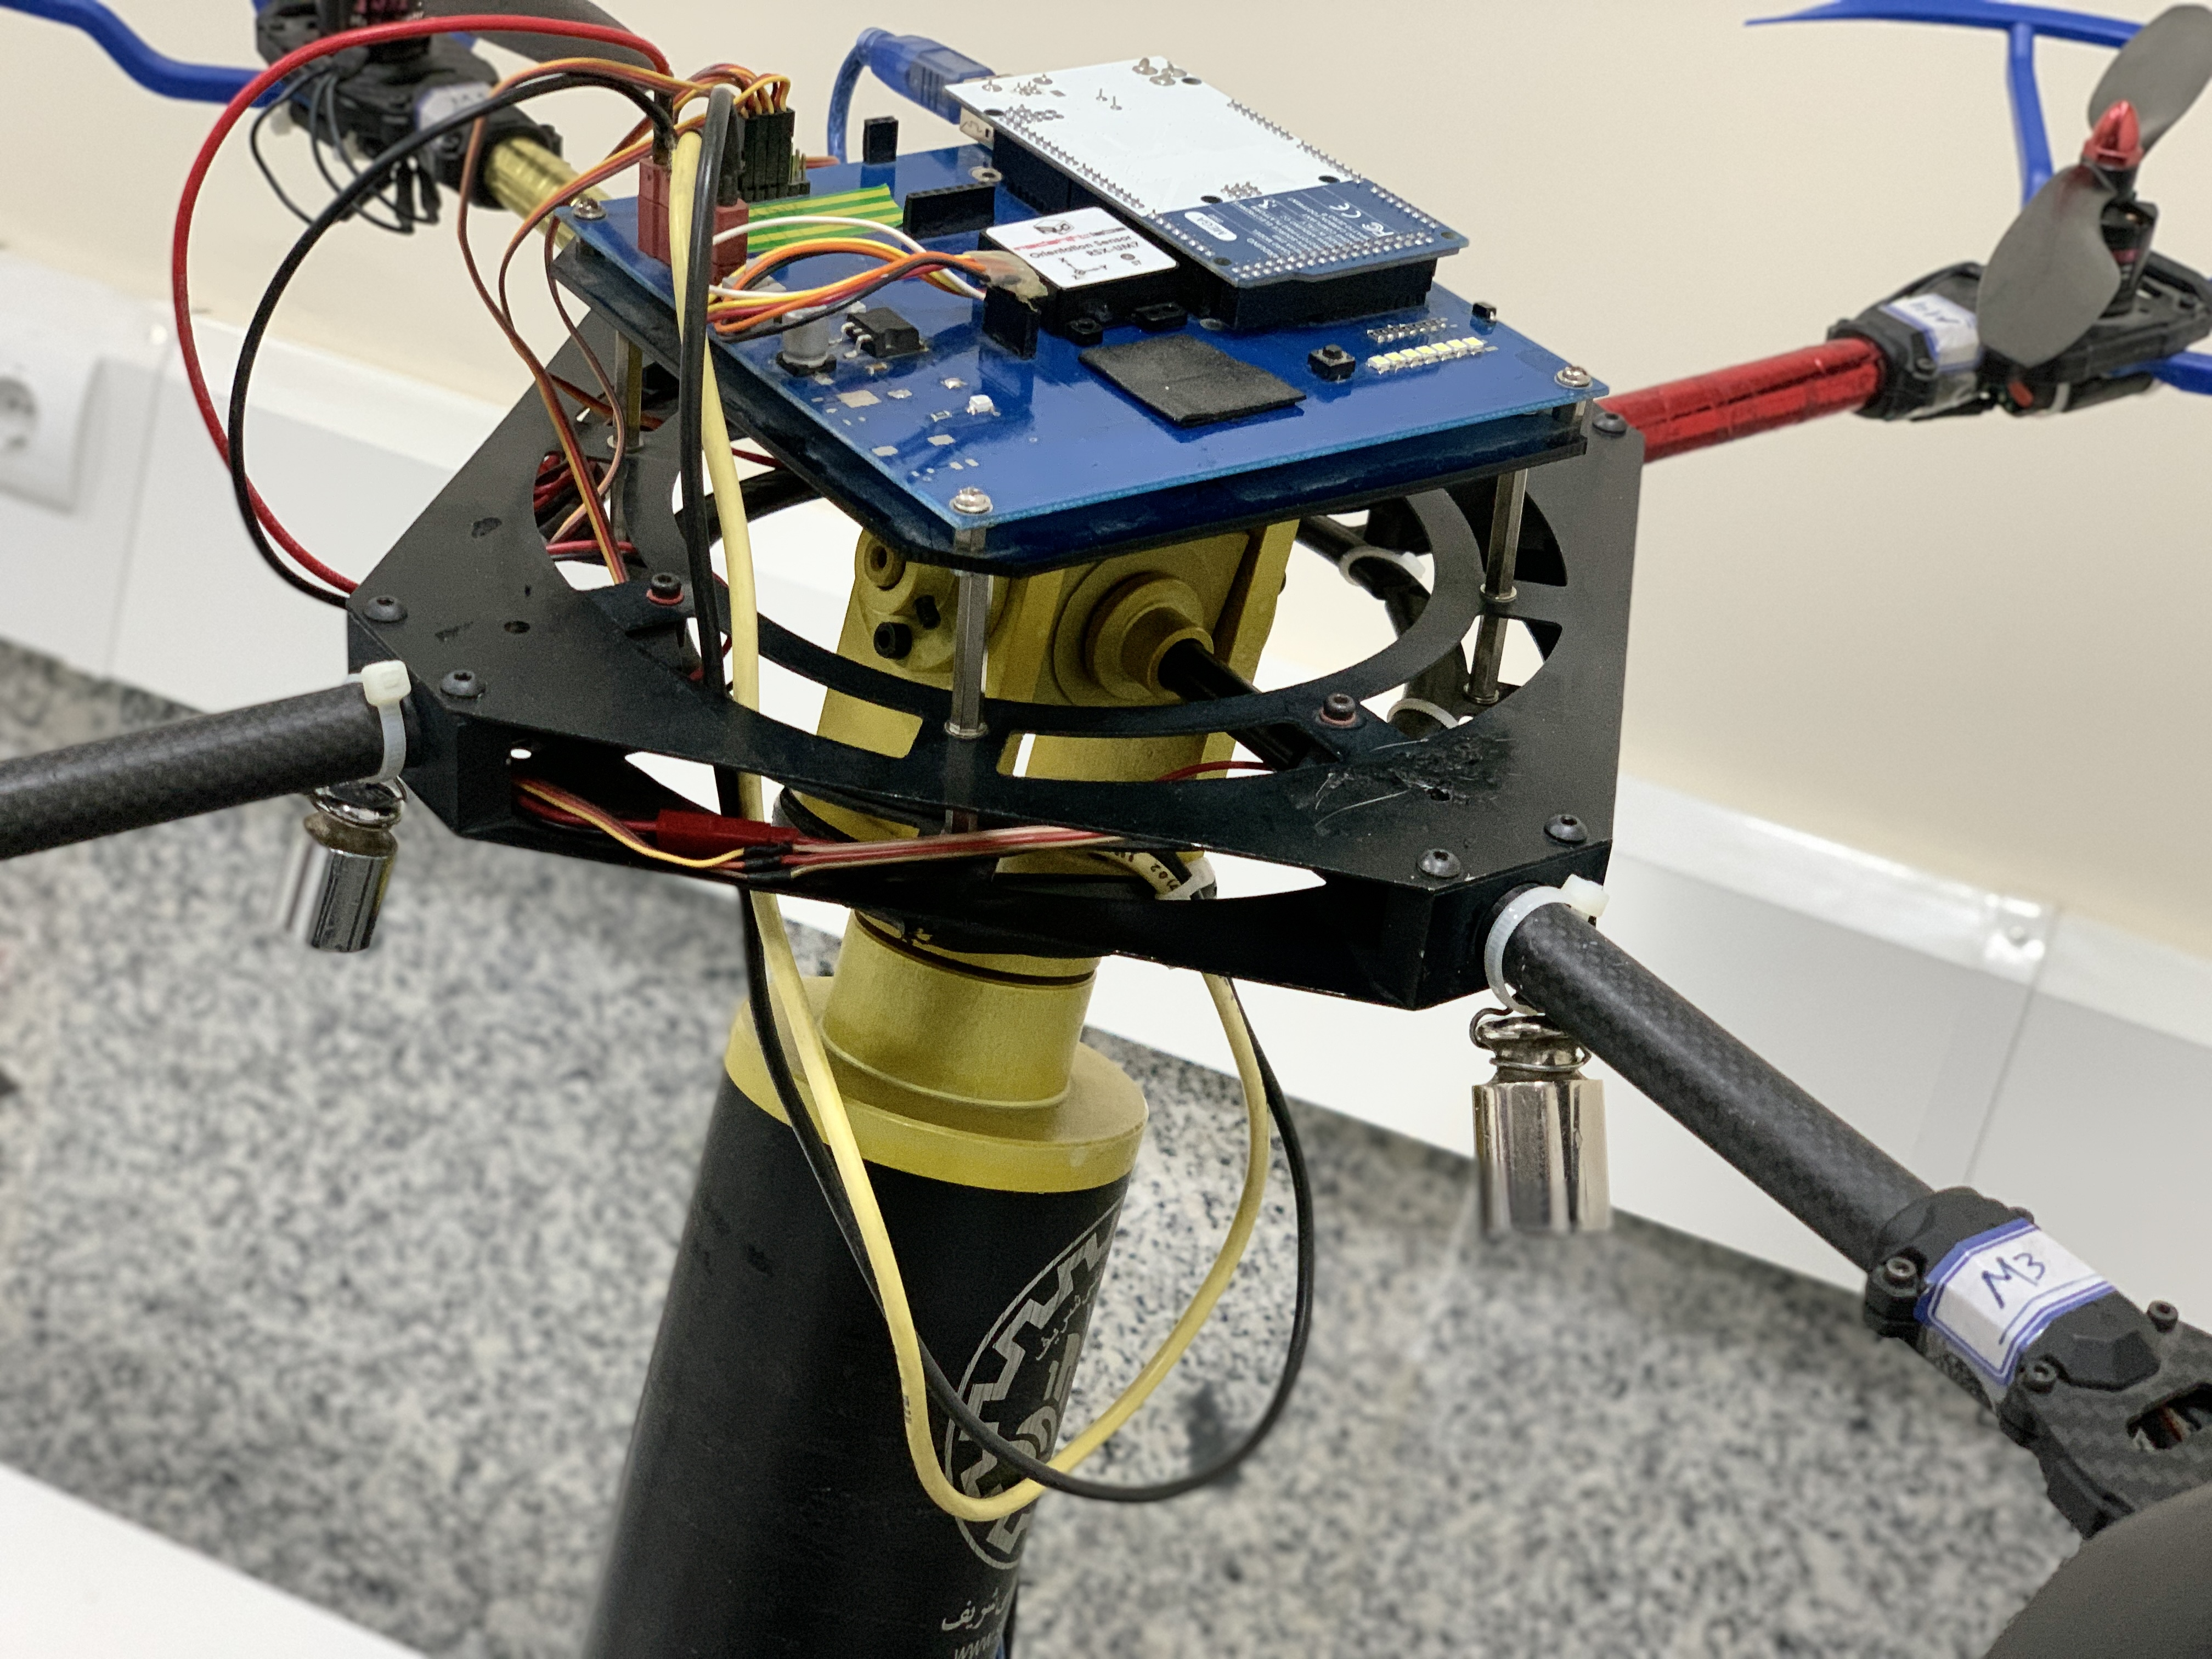
\includegraphics[width=0.45\textwidth]{../Figure/implementation/weight/Quad_with_weight.jpg}
    \caption{Quadrotor 3-DoF platform with added weights.} %%%? is it okey
~\label{fig:quadrotor_with_weight}
%  \end{figure}
%  \begin{figure}[H]
    \centering
    \subfloat[\label{fig:weight_roll}]{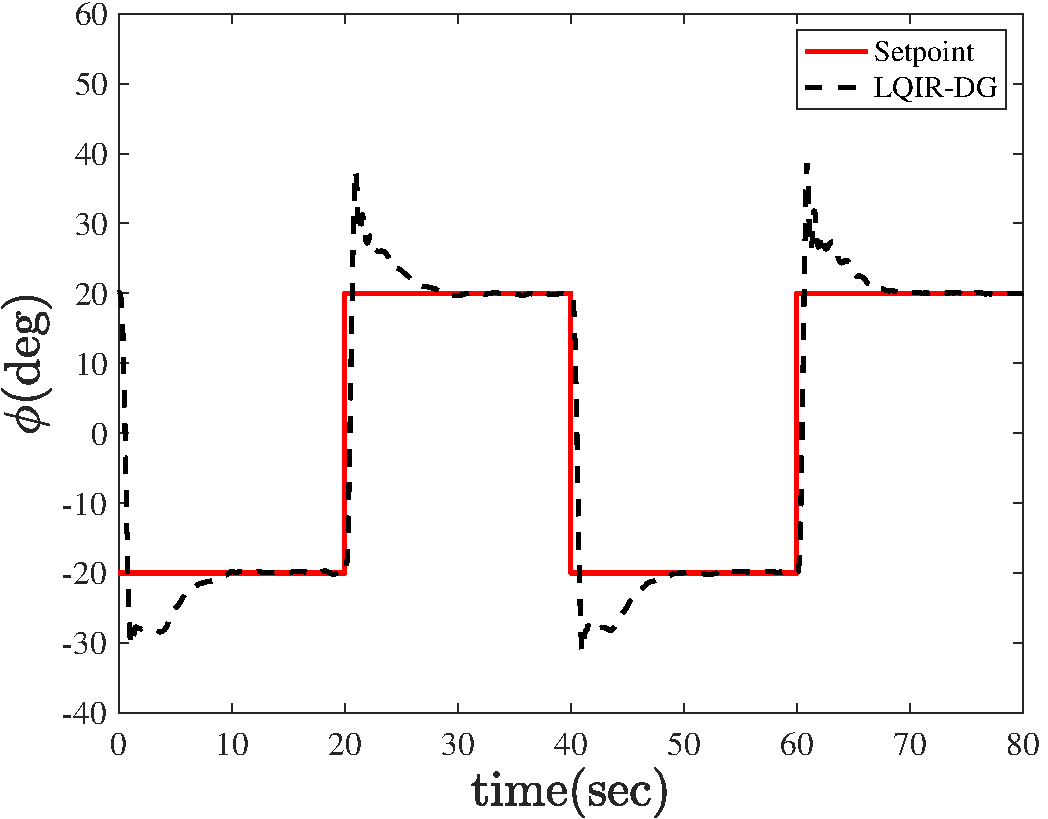
\includegraphics[width=.45\linewidth]{../Figure/implementation/weight/lqidg_roll_20}}\subfloat[\label{fig:weight_pitch}]{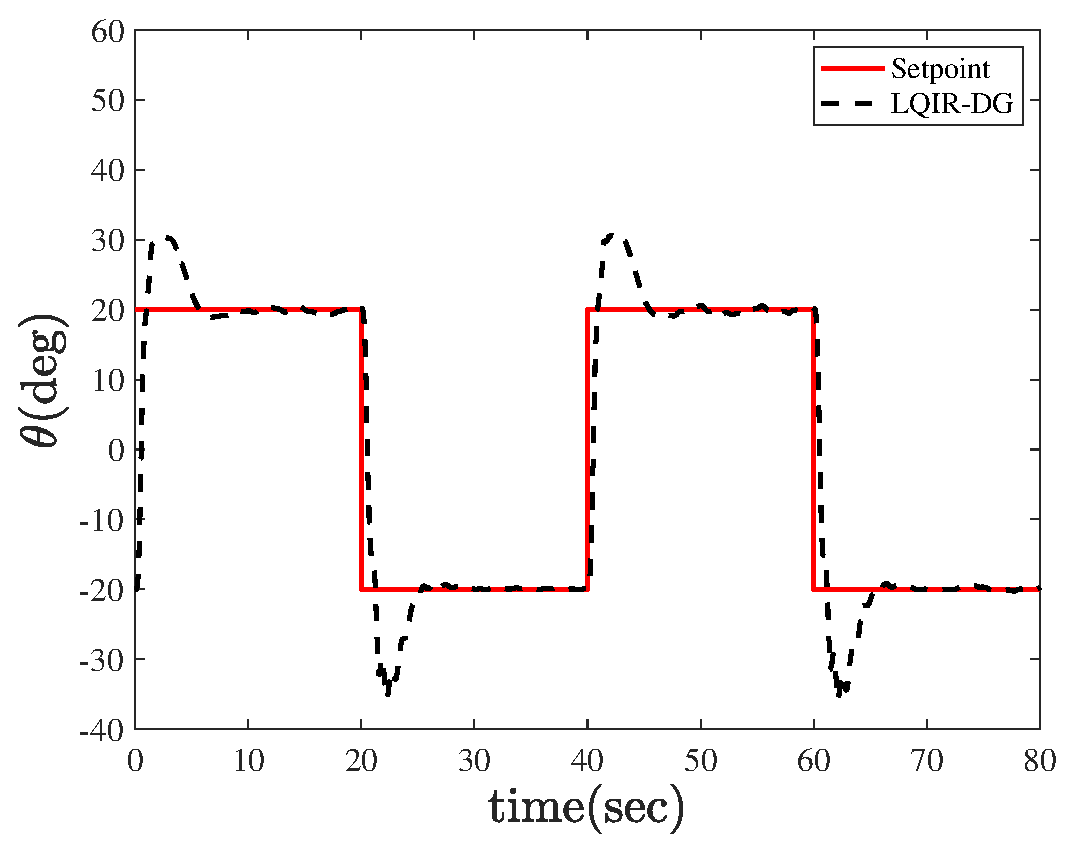
\includegraphics[width=.45\linewidth]{../Figure/implementation/weight/lqidg_pitch_20}
    }
    \hfill
    \subfloat[\label{fig:omega_weight}]{\includegraphics[width=.25\linewidth]{../Figure/implementation/weight/lqidg_Omega_1}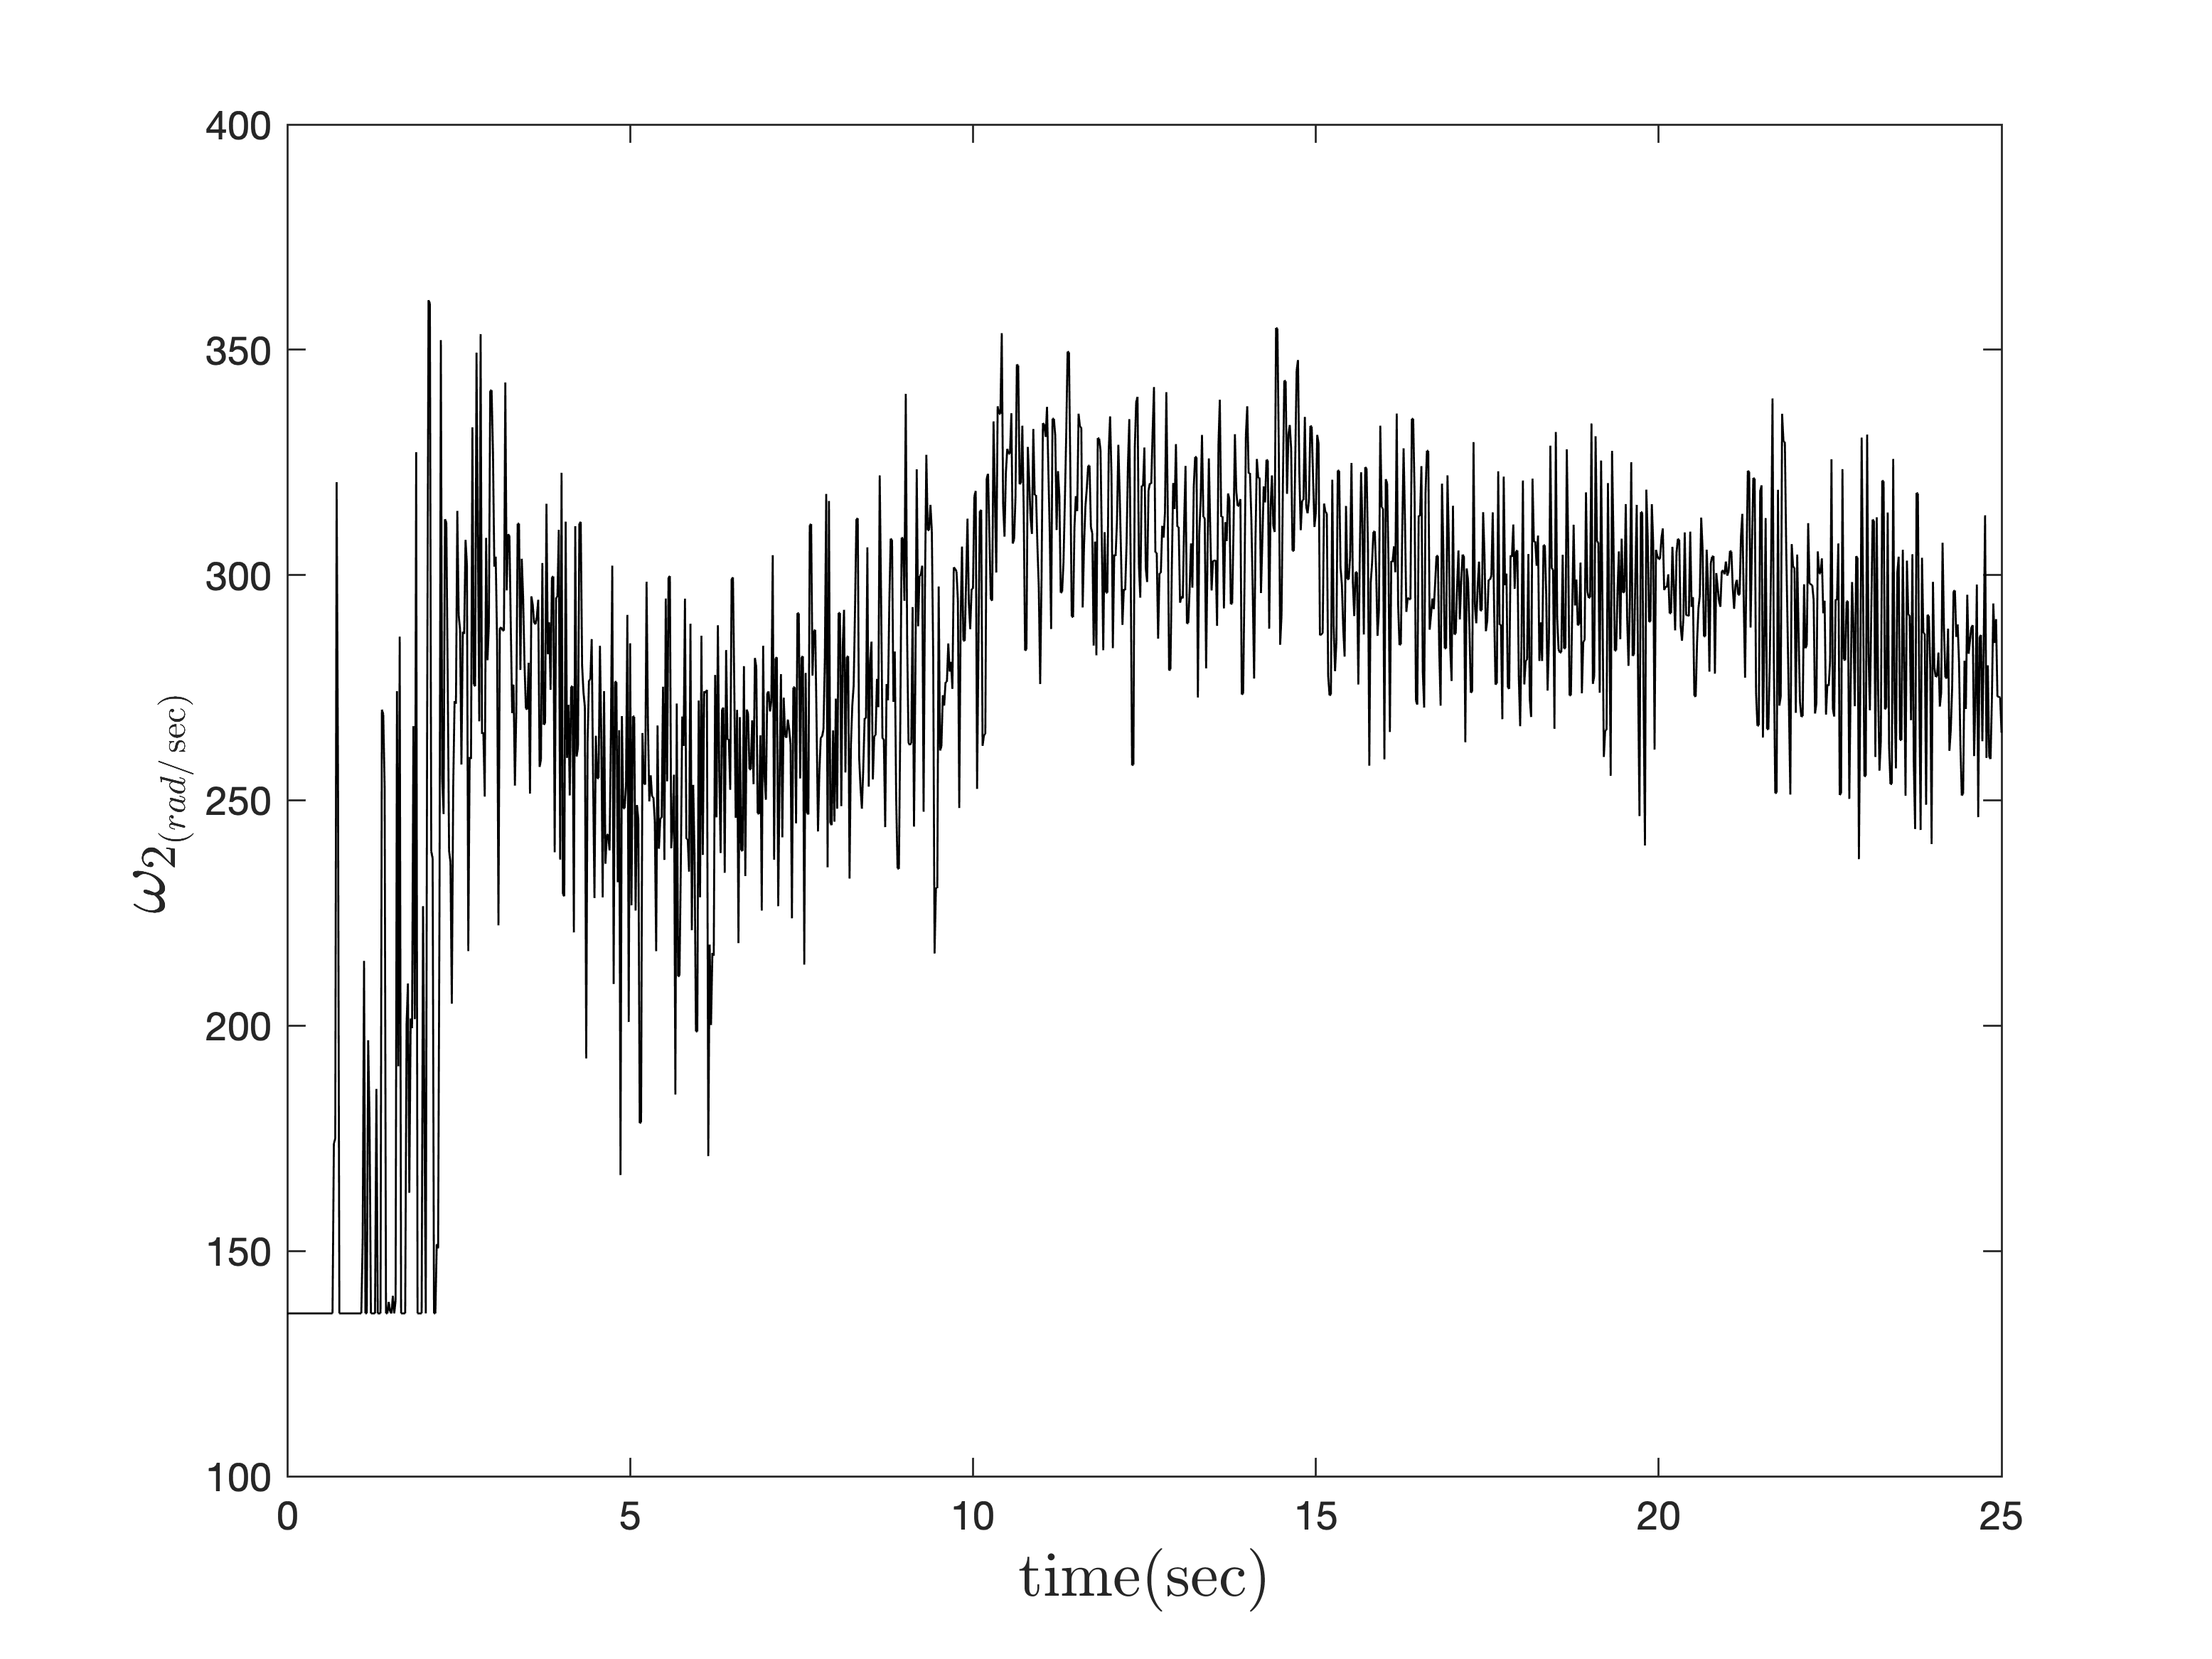
\includegraphics[width=.25\linewidth]{../Figure/implementation/weight/lqidg_Omega_2}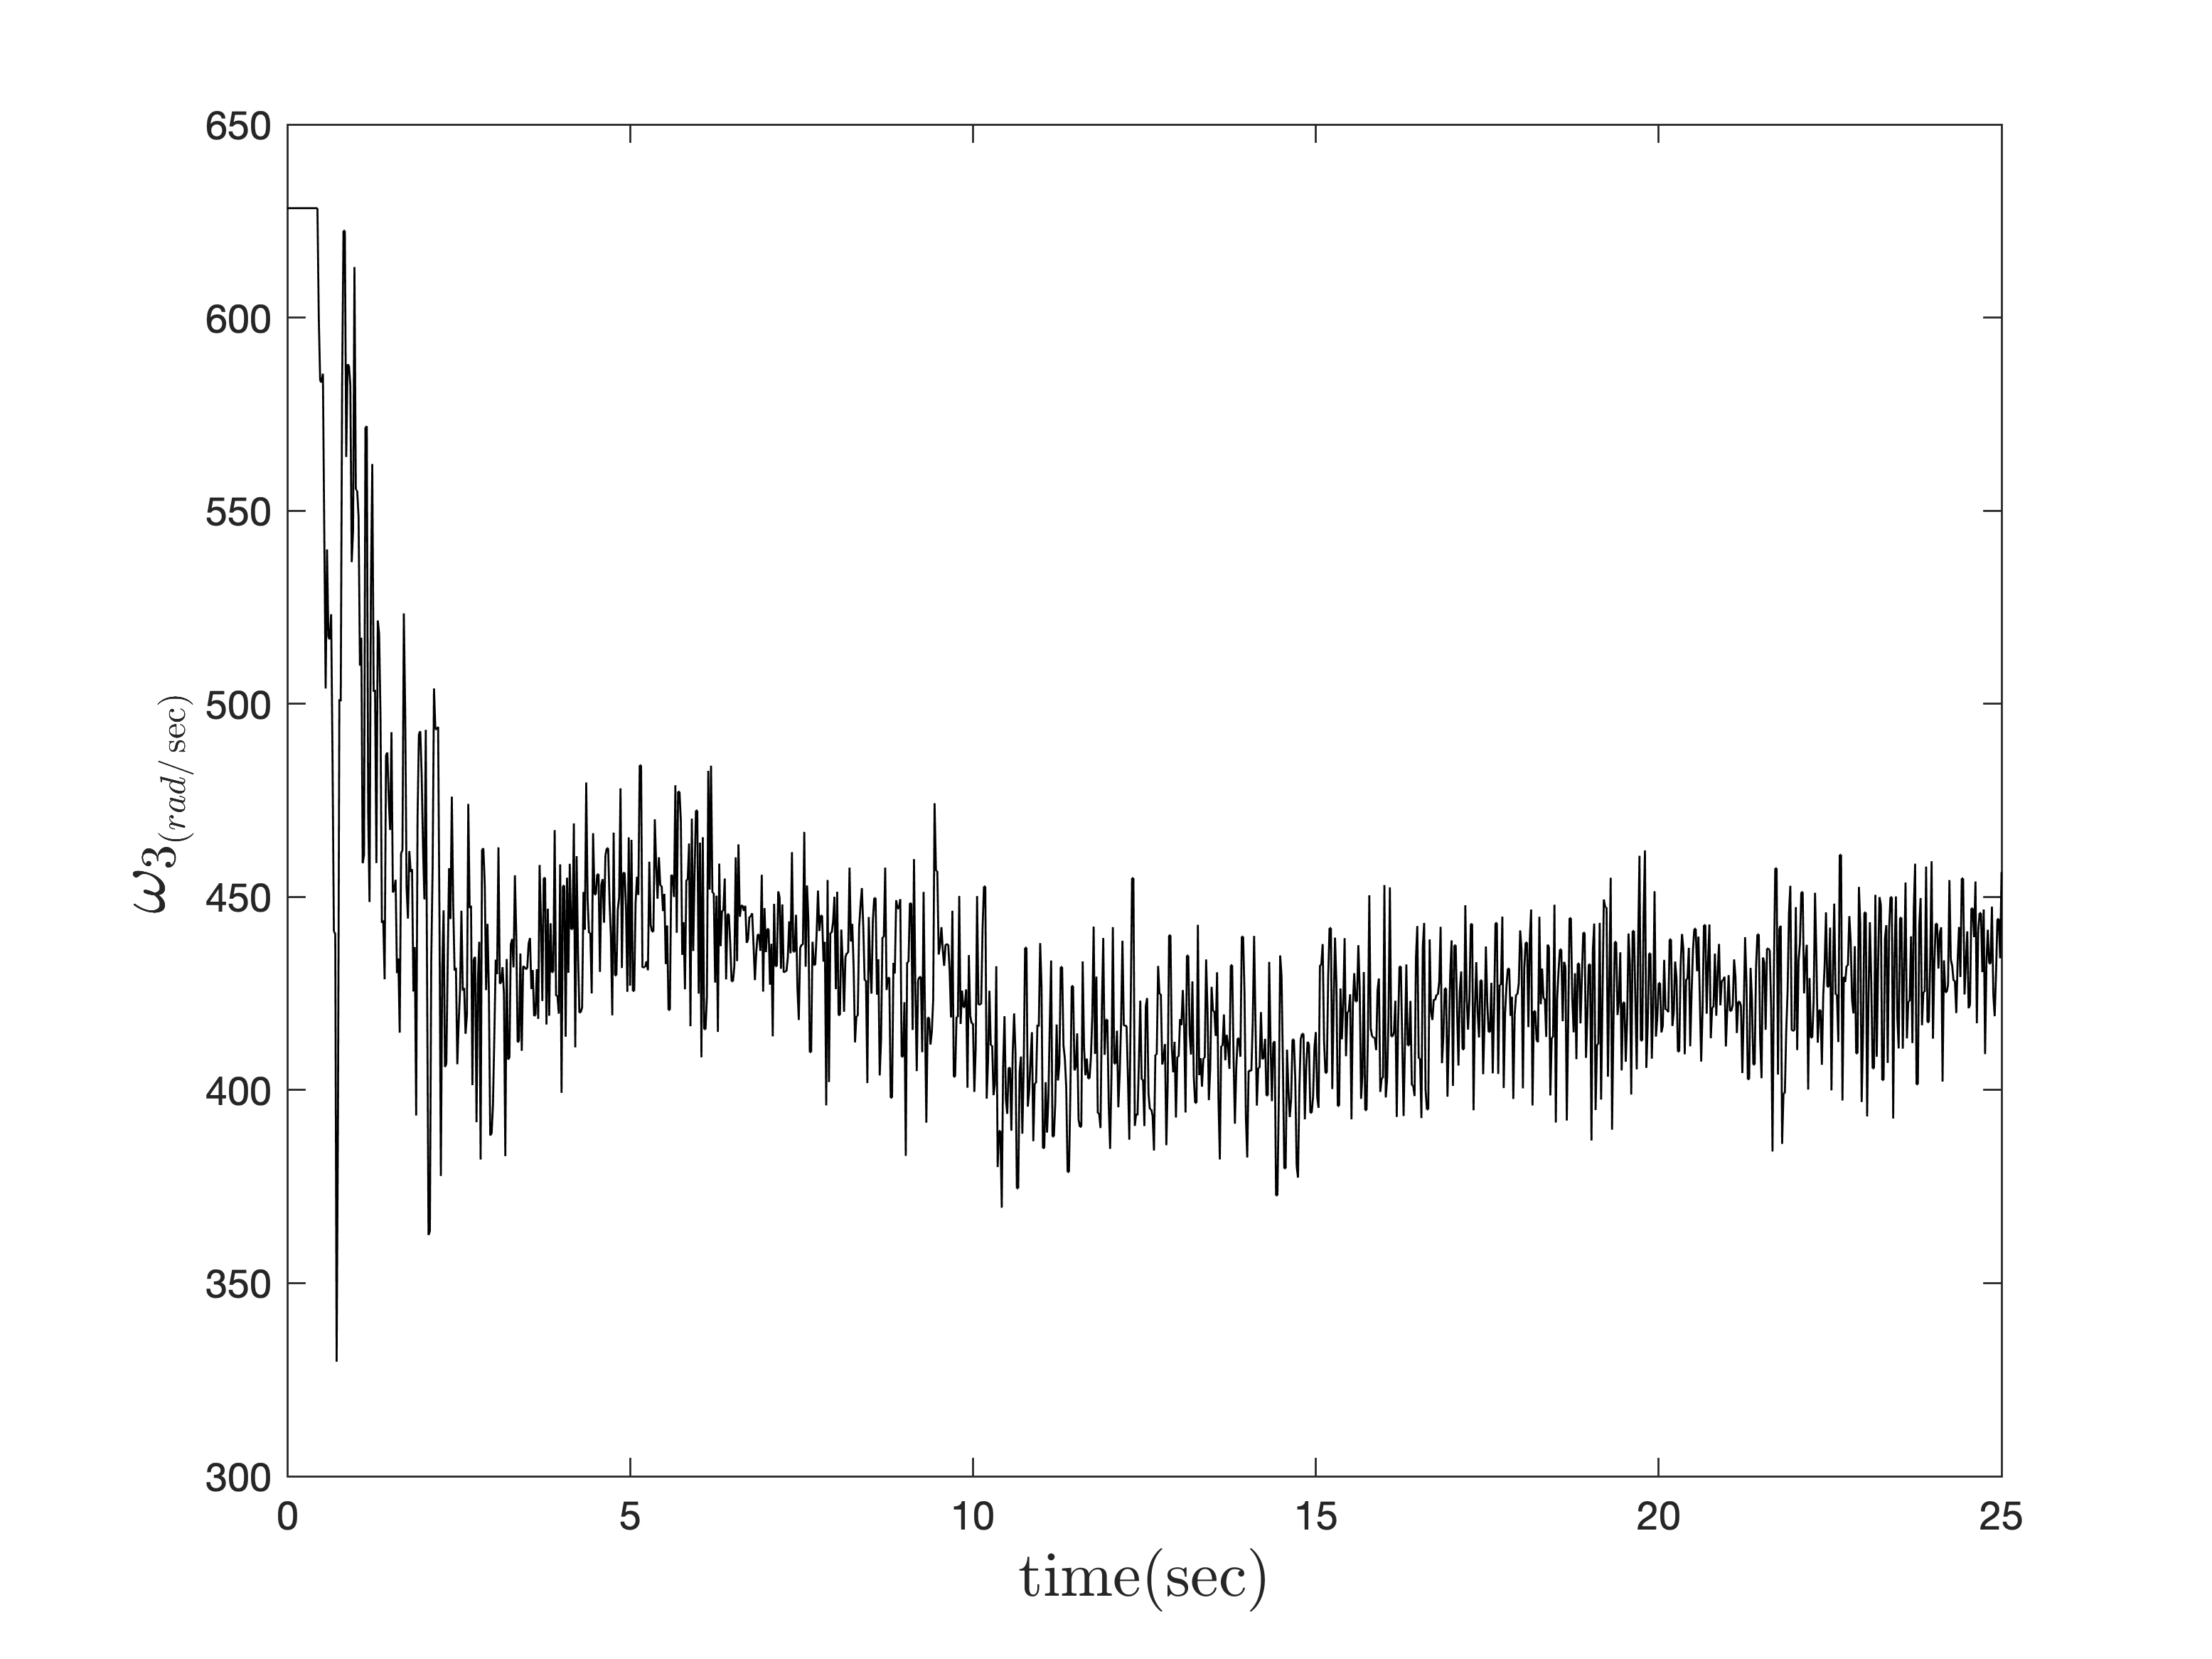
\includegraphics[width=.25\linewidth]{../Figure/implementation/weight/lqidg_Omega_3}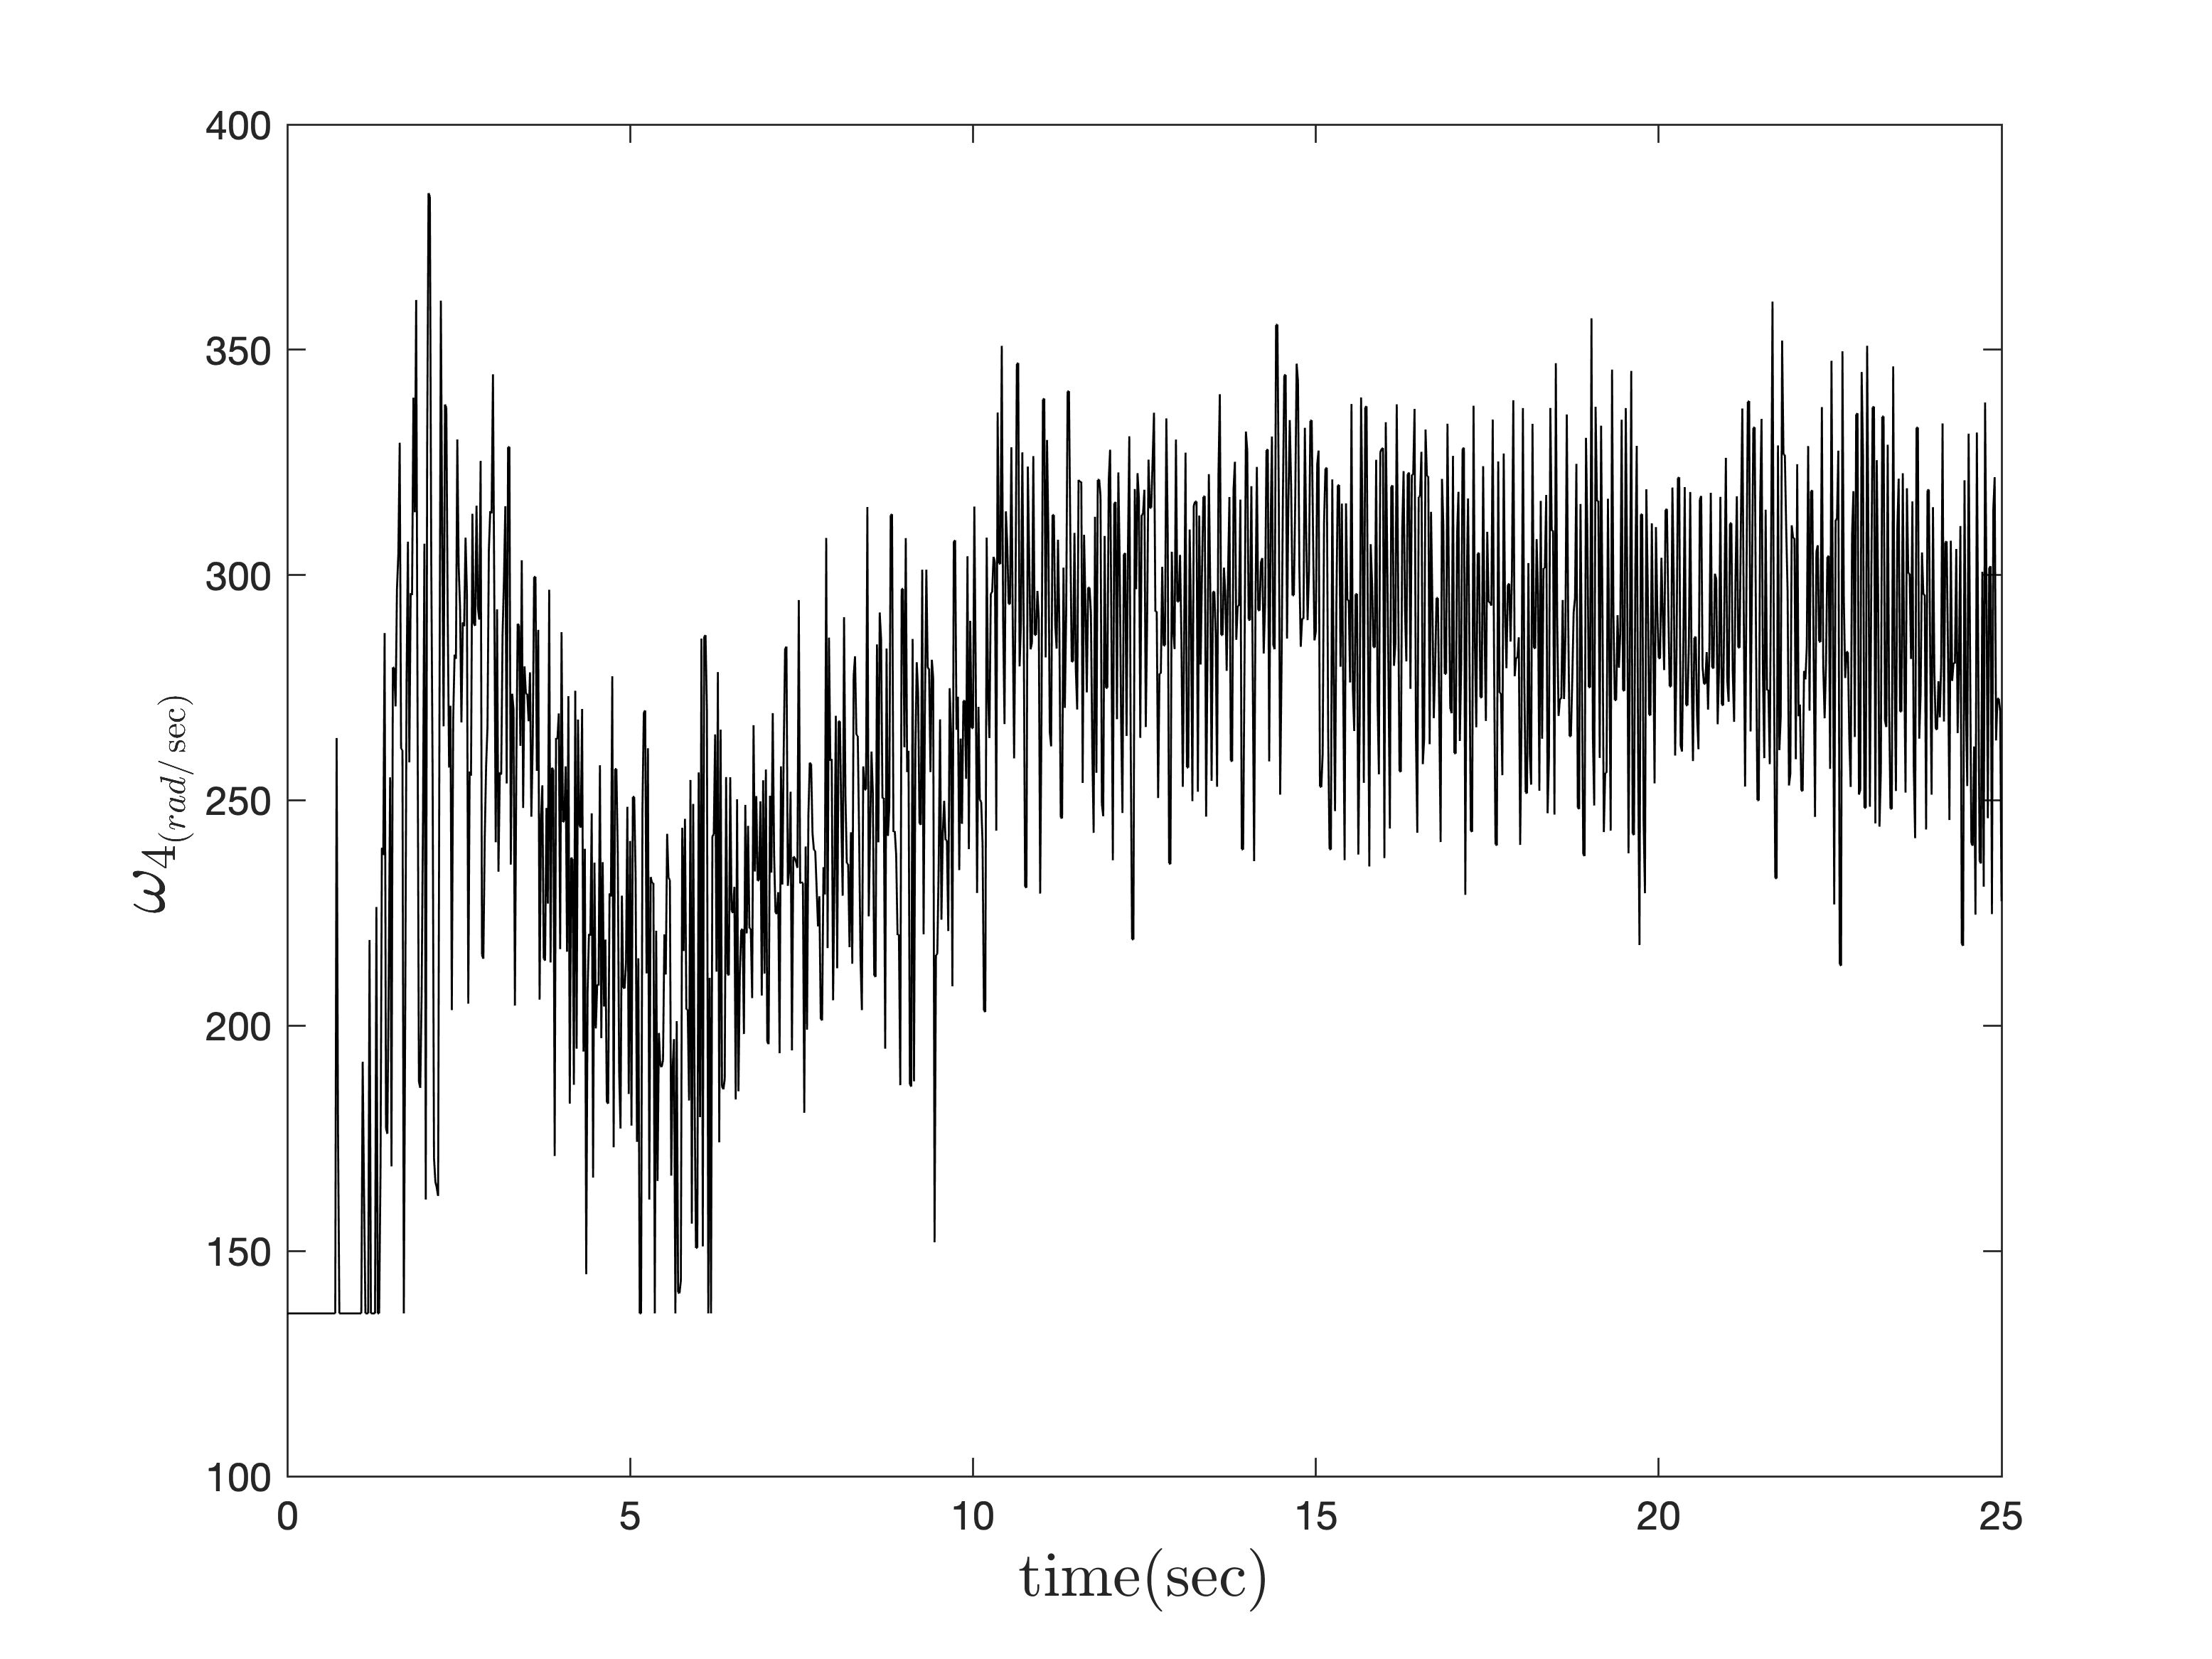
\includegraphics[width=.25\linewidth]{../Figure/implementation/weight/lqidg_Omega_4}}
    \caption{Comparison of actual roll and pitch angles with desired values, when the modeling uncertainty is present.}
    \label{fig:weight}
\end{figure}
\subsubsection{Comparison with the Control Strategies}
\noindent Figure~\ref{fig:compare} compares the LQIR-DG controller performance with the PID controller and variant of the LQR strategies such as the LQR and LQIR. 
Moreover, the box plot of all controllers is plotted in Figure~\ref{fig:compare_boxplot} for the cost function, introduced in equation \eqref{eq:min_max_cost_function}. %%%? two controller side by side
The median of Root Mean Square Error (RMSE) is shown in the crossline in the box plot.
Moreover, the LQIR-DG controller performance with famous disturbance rejection methods, such as Active Disturbance Rejection Control (ADRC) \cite{CHENG2023} and Disturbance Observer-Based Control (DOBC) \cite{AGHAYAN202320} are compared in Figure \ref{fig:compare_adrc}, when the input disturbances occur according to equation \eqref{eq:disturbance}. For the cost function, denoted in equation \eqref{eq:min_max_cost_function}, the box plot of these robust controllers is illustrated in Figure \ref{fig:compare_boxplot_ADR}. 
These results indicate that the proposed controller is able to provide rapid convergence, excellent transient, and robustness to disturbances relative to other controllers for attitude control of the experimental platform.

\begin{figure}[H]
    \centering
    \subfloat[\label{fig:all_roll}]{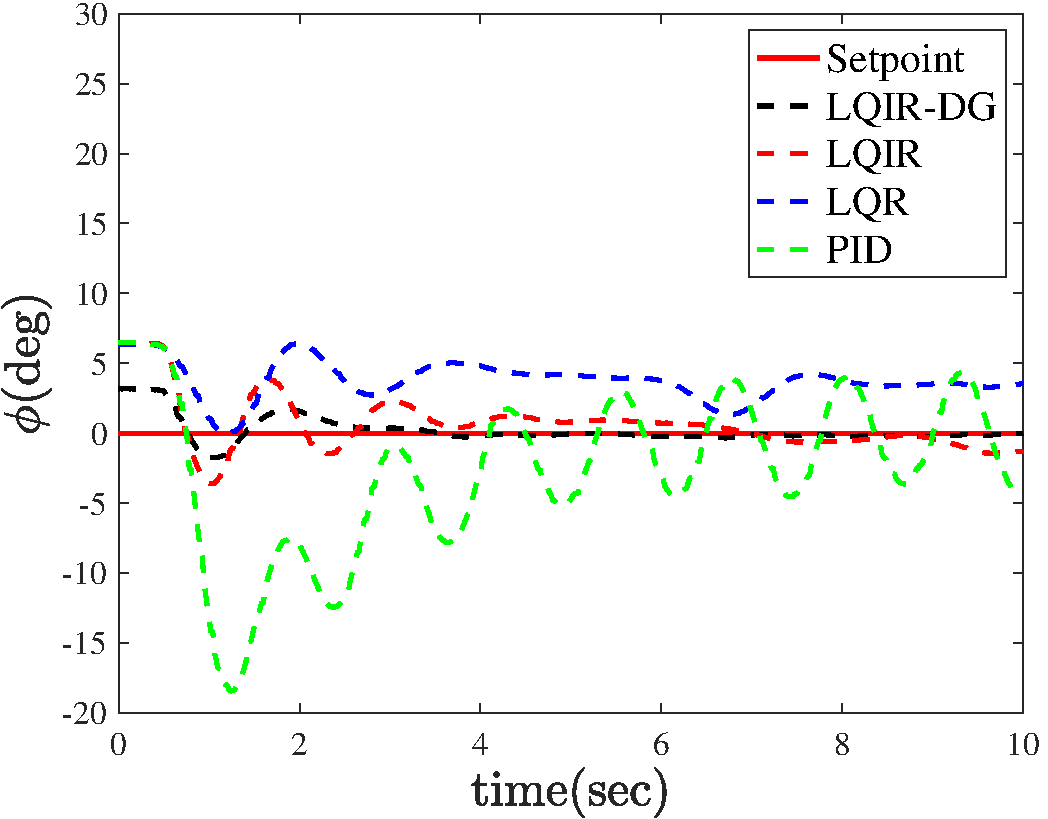
\includegraphics[width=.49\linewidth]{../Figure/implementation/lqidgvslqr/roll}}\subfloat[\label{fig:all_pitch}]{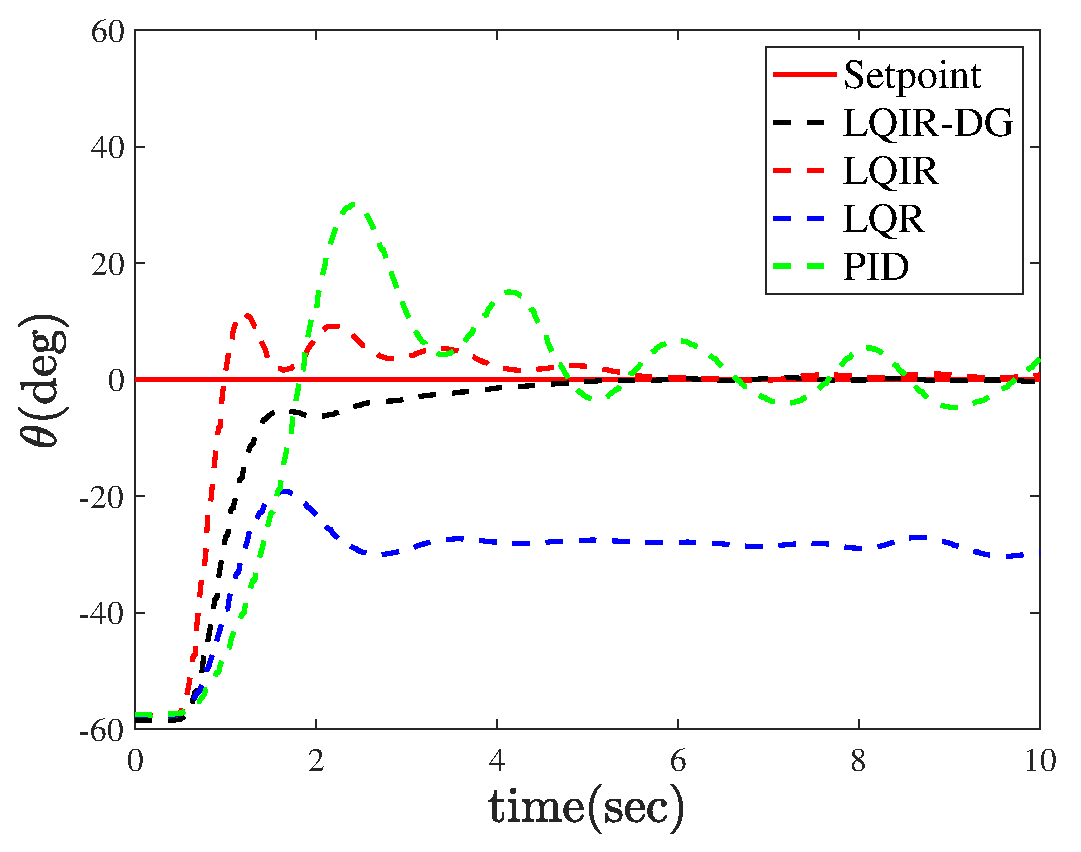
\includegraphics[width=.49\linewidth]{../Figure/implementation/lqidgvslqr/pitch}
    }
    \caption{Comparison of LQIR-DG structure with the variant of LQR and PID in regulation problem:~\ref{sub@fig:all_roll} roll angle~\ref{sub@fig:all_pitch} pitch angle.}
    \label{fig:compare}
\end{figure}

\begin{figure}[H]
    \centering
    {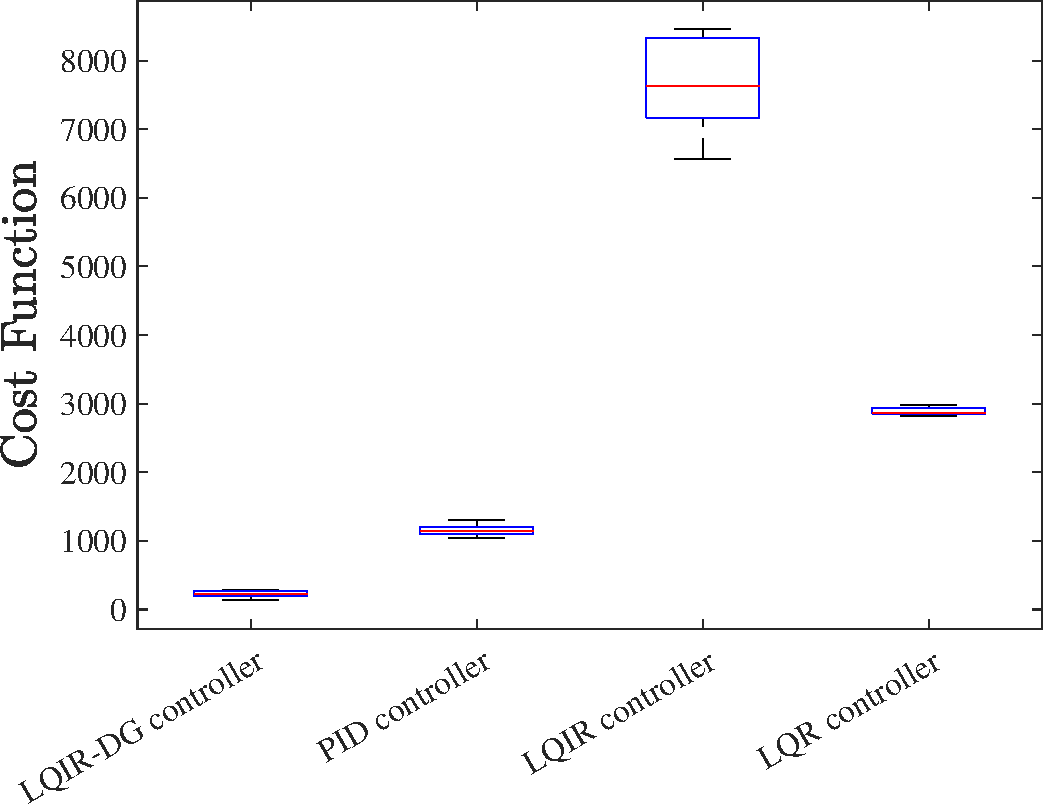
\includegraphics[width=.55\linewidth]{../Figure/implementation/box_plot/lqidgvsboxplot}
    }
    \caption{Box plot of LQIR-DG, LQR, LQIR, and PID controllers.}
    \label{fig:compare_boxplot}
\end{figure}


\begin{figure}[H]
    \centering
    \subfloat[\label{fig:ADR_vs}]{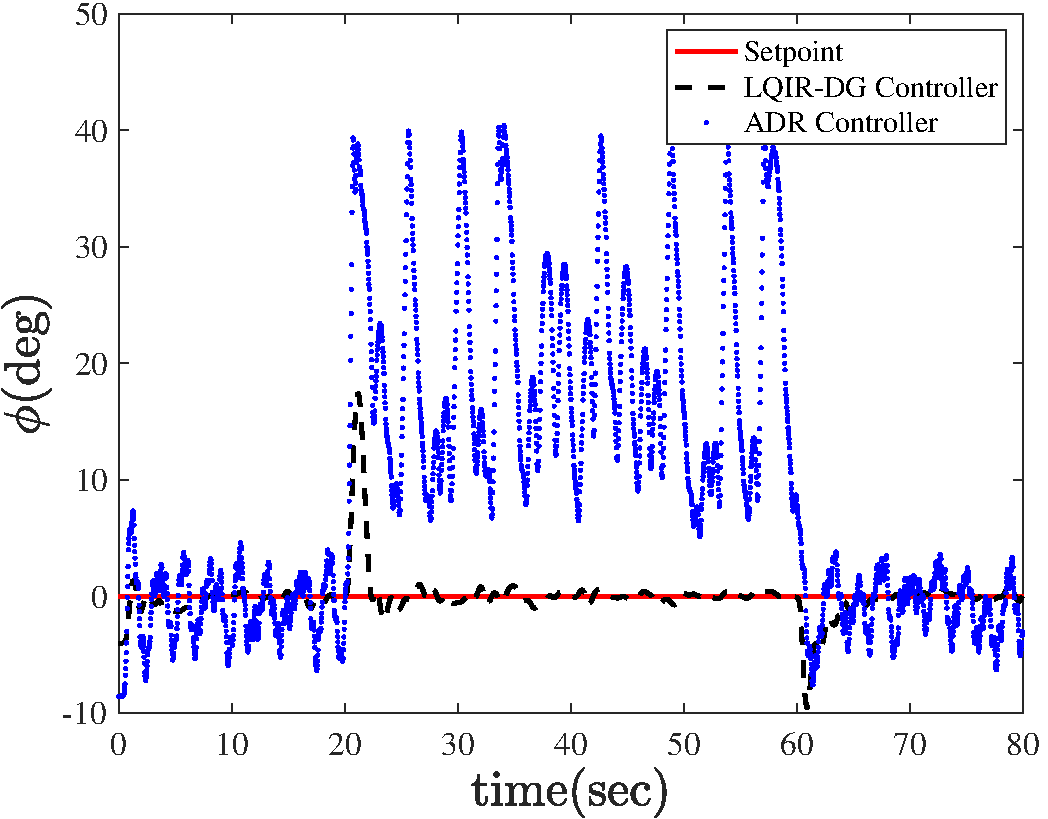
\includegraphics[width=.45\linewidth]{../Figure/implementation/disturbance/lqidg_dis_ADR_roll}{\includegraphics[width=.45\linewidth]{../Figure/implementation/disturbance/lqidg_dis_ADR_pitch}}
    }
    \hfill
    \subfloat[\label{fig:DOB_vs}]{\includegraphics[width=.45\linewidth]{../Figure/implementation/disturbance/lqidg_dis_DOB_roll}\includegraphics[width=.45\linewidth]{../Figure/implementation/disturbance/lqidg_dis_DOB_pitch}
    }
    \caption{Comparison of LQIR-DG structure with the famous disturbance rejection methods: \ref{sub@fig:ADR_vs}  Active Disturbance Rejection Control (ADRC) \ref{sub@fig:DOB_vs} Disturbance Observer-Based Control (DOBC).}
    \label{fig:compare_adrc}
\end{figure}

\begin{figure}[H]
    \label{fig:compare_boxplot_ADR}
    \centering
    {\includegraphics[width=.5\linewidth]{../Figure/implementation/box_plot/lqidgvsboxplot_ADR}
    }
    \caption{Box plot of LQIR-DG, ADRC, and DOBC methods.}
    \label{fig:compare_boxplot_ADR}
\end{figure}

\section{Conclusion}\label{sec:conclusion}
\vspace{-0.15cm}
\noindent In this paper, the linear quadratic integral differential game approach, was used in real-time for attitude control of the platform quadrotor. %%%? for quadrotor
For the implementation of the controller structure, an accurate dynamic model was considered for the experimental platform.
Then, the model parameters were identified using the NSL method.
For evaluation of the proposed method, the regulation and tracking proposed were successfully performed.
Moreover, the ability of the proposed method was investigated in the rejection of the input disturbance and modeling error in the experimental platform.
Finally, a comparison
was also performed between the results of classical PID variations of LQR and the robust structures with the proposed method.
The implementation results illustrated the excellent performance of the LQIR controller based on the game theory approach in attitude control for the quadrotor platform.
However, one challenge in applying this method to the 3-DOF quadrotor experimental setup was the presence of noise and errors of the AHRS sensor. It was calibrated before a run of the algorithm. One another challenge was in implementing the controller. Since, this controller required a desired trajectory, it was programmed on the Arduino Mega2560 board using the embedded coder before a run of the algorithm.


% \section{The Non-cooperative Game}

% The Uncertain Non-cooperative Game section introduces model uncertainty into the dynamic non-cooperative game framework. The rationale is that in real-world situations, agents or players operate based on imperfect models of the environment. Rather than optimizing based on a detailed but inaccurate model, it makes more sense for players to use a simple model but incorporate robustness to specification errors.  

% This is modeled by adding a malevolent disturbance input to the system dynamics to represent model mismatch. Each player $i$ has their own expectation about this disturbance, and copes with it by considering a worst-case scenario.  

% Specifically, the system dynamics become:
% \begin{align}
% \dot{x} = Ax + B_1u_1 + B_2u_2 + Ew
% \end{align}
% where $w$ is the disturbance input.  

% Each player $i$ minimizes a cost function that includes a penalty on the disturbance $w$: 
% \begin{align}
% J_i = \int (x^\top Q_i x - w^\top V_i w) dt
% \end{align}
% where $V_i > 0$ represents player $i$'s aversion to model risk. The higher $V_i$ is, the more conservative player $i$ is regarding mismatches between their model and reality.

% The problem is to find robust open-loop and feedback strategies $u_1, u_2$ that form a Nash equilibrium even under worst-case disturbance $w$. Sufficient conditions are provided in terms of coupled Riccati equations. For instance, in the open-loop infinite horizon case, the strategies are robust if:
% \begin{enumerate}
% \item A set of algebraic Riccati equations have a strongly stabilizing solution 
% \item A pair of decoupled Riccati equations have a stabilizing solution
% \end{enumerate}
% This ensures the open-loop strategies $u_1, u_2$ form a saddle point equilibrium for the min-max problem. Similar results are presented for the feedback case.  

% Overall, this section incorporates model uncertainty into the standard LQ differential game framework in a tractable way. The min-max optimization represents each player's robustness mindset and desire to guard against model risk. The sufficient conditions help determine when robust equilibria exist.

% \section{Proof of Robust Open-Loop Nash Equilibrium}

% Here is a proof sketch showing how the min-max optimization with model uncertainty leads to coupled Riccati equations to find robust Nash equilibria:

% \begin{proof}
% Consider the infinite horizon open-loop differential game with dynamics and cost function as defined above.  

% Let $u_i(t) = -R_{ii}^{-1}B_i^\top P_i x(t)$ be the open-loop control strategies, where $P_i$ satisfies an algebraic Riccati equation. 

% Let $w(t) = V_i^{-1}E^\top P_i x(t)$ be the worst-case disturbance input.

% Substituting these into the dynamics and cost function $J_i$, the cost becomes: 

% \begin{align}
% J_i = \int x^\top P_i x dt
% \end{align}

% Taking the derivative of $V_iJ_i$ along the system dynamics gives: 

% \begin{align}
% \frac{dJ_i}{dt} = x^\top (Q_i + A^\top P_i + P_iA - P_i(S_i - M_i)P_i)x
% \end{align}

% Where $S_i = BR_i^{-1}B_i^\top$ and $M_i = EV_i^{-1}E^\top$.

% For $J_i$ to be non-increasing, the term in parentheses must be negative semidefinite. This gives the Riccati equation: 

% \begin{align}
% 0 = Q_i + A^\top P_i + P_iA - P_i(S_i - M_i)P_i
% \end{align}

% Additionally, for stability the closed loop $A - S_iP_i + M_iP_i$ must be stable.  

% If both players' $P_i$ satisfy such Riccati equations, with stability, then neither player can improve their cost $J_i$ by deviating from $u_i$ or $w_i$. Thus the strategies form a Nash equilibrium.

% The key steps are:
% \begin{enumerate}
% \item Guess the optimal strategies in terms of $P_i$
% \item Substitute into dynamics and cost  
% \item Take derivatives and require $dJ_i/dt \leq 0$
% \item This leads to a Riccati equation that $P_i$ must satisfy
% \item If both players' $P_i$ satisfy the Riccati equations, then neither has incentive to deviate, giving a NE.
% \end{enumerate}

% So the Riccati equations arise from the first-order optimality conditions on the min-max problem to ensure a saddle point equilibrium. Solving them is both necessary and sufficient for robust open-loop Nash equilibrium.
% \end{proof}









% Here is the proof and analysis for the two player case of the system versus a disturbance:

% \section{Two Player Game: System vs Disturbance}

% In the simplest case, we can model the uncertain game as having just two players - the system controller, and a disturbance input representing model mismatch. 

% The system dynamics are:

% \begin{align}
% \dot{x} = Ax + Bu + Ew
% \end{align}

% Where $u$ is the control input and $w$ is the disturbance.

% The system controller minimizes the quadratic cost:

% \begin{align}
% J = \int (x^\top Q x + u^\top R u) dt
% \end{align}

% And the disturbance maximizes: 

% \begin{align}
% J_d = -\int w^\top V w dt
% \end{align}

% Where $V \succ 0$ represents aversion to model uncertainty.

% To find the robust strategies $u^*, w^*$, we posit:

% \begin{align}
% u^* &= -R^{-1}B^\top Px \\
% w^* &= V^{-1}E^\top Px
% \end{align}

% Where $P$ satisfies the Riccati equation: 

% \begin{align}
% 0 &= Q + A^\top P + PA - PBR^{-1}B^\top P + PEV^{-1}E^\top P \\
% 0 &= Q + A^\top P + PA - P(S - M)P
% \end{align}

% With $S=BR^{-1}B^\top, M=EV^{-1}E^\top$. 

% If $P$ satisfies this equation with $A-SP+MP$ stable, then $u^*, w^*$ form a robust Nash equilibrium.

% \begin{proof}{Two player robust Nash equilibrium}
% Follows similar steps as general proof by substituting strategies into dynamics and cost functions. The strategies being mutual best responses leads to the Riccati equation characterizing robust NE.
% \end{proof}

% So the two player case provides intuitive interpretation and simplifies analysis, while retaining the key model uncertainty concepts and use of coupled Riccati equations.


% Here is the proof and analysis for the two player case with coupled Riccati equations:

% \section{Two Player Game with Coupled Riccati Equations}

% We consider the two player game between the system and disturbance. The dynamics and cost functions are:

% \begin{align}
% \dot{x} &= Ax + Bu + Ew\\
% J &= \int (x^\top Q x + u^\top R u) dt\\ 
% J_d &= -\int w^\top V w dt
% \end{align}

% To find the robust strategies $u^*, w^*$, we now posit:

% \begin{align}
% u^* &= -R^{-1}B^\top P_1 x\\ 
% w^* &= V^{-1}E^\top P_2 x
% \end{align}

% Where $P_1, P_2$ satisfy the coupled Riccati equations:

% \begin{align}
% 0 &= A^\top P_1 + P_1 A - P_1 BR^{-1} B^\top P_1 + P_1 E V^{-1}E^\top P_2 + Q\\
% 0 &= A^\top P_2 + P_2 A + P_2 E V^{-1}E^\top P_2 - P_2 BR^{-1}B^\top P_1 
% \end{align}

% If $P_1,P_2$ satisfy these equations and render $A-BR^{-1}B^\top P_1 + EV^{-1}E^\top P_2$ stable, then $u^*, w^*$ form a robust Nash equilibrium.

% \begin{proof}{Two player coupled Riccati robust NE}
% Substituting the strategies into the dynamics and cost functions, and taking derivatives, leads to the coupled Riccati equations arising from mutual best response conditions. Solving the equations provides the robust NE strategies.
% \end{proof}

% The coupling represents the interdependence between the system controller's and disturbance's strategies. Solving the set of equations provides both players' robust optimizing strategies in feedback form.




%% The Appendices part is started with the command \appendix;
%% appendix sections are then done as normal sections
%% \appendix

%% \section{}
%%~\label{}

%% If you have a bib database file and want BibTeX to generate the
%% bib items, please use
%%
% \vspace{-0.3cm}
\bibliographystyle{elsarticle-num} 
 \bibliography{refs}

 % appendix: linearization
\newpage
\appendix
\section{Linearization Proof of the Quadrotor Nonlinear Model }
\label{sec:linearization}
Here, the nonlinear model of the quadrotor, described in equations \eqref{eq:eq_of_motion_start1}-\eqref{eq:eq_of_motion_end1}, are linearized using first-order Taylor series expansion about the equilibrium points $(\boldsymbol{x}^* \text{ and } \boldsymbol{u}^*)$. For this purpose, the linear form of the nonlinear system denoted as $\dot{\boldsymbol{x}} = \boldsymbol{f}(\boldsymbol{x}, \boldsymbol{u})$, is computed as
\begin{equation}
    \dot{\boldsymbol{x}} = \boldsymbol{\mathrm{A}}
\boldsymbol{x} + \boldsymbol{\mathrm{B}}\boldsymbol{u}
\end{equation}
where $\boldsymbol{\mathrm{A}}$ and $\boldsymbol{\mathrm{B}}$ are, respectively, the states and input matrices, computed as \cite{simon2006optimal}
\begin{equation}
    \mathbf{A} = \left.\dfrac{\partial \mathbf{f}}{\partial \mathbf{x}}\right|_{\boldsymbol{{\mathrm{x}}}^*, \boldsymbol{{\mathrm{u}}}^*}
\end{equation}
\begin{equation}
    \mathbf{B} = \left.\dfrac{\partial \mathbf{f}}{\partial \mathbf{u}}\right|_{\boldsymbol{{\mathrm{x}}}^*, \boldsymbol{{\mathrm{u}}}^*}
\end{equation}
To linearize the nonlinear model of the quadrotor around the equilibrium points $(\boldsymbol{x}^* = 0 \text{ and } \boldsymbol{u}^* = 0)$, the Jacobian matrix of nonlinear model, denoted in equations \eqref{eq:eq_of_motion_start1}-\eqref{eq:eq_of_motion_end1}, is expressed as:

\begin{align}
    \mathbf{A} =& \left.\dfrac{\partial \mathbf{f}}{\partial \mathbf{x}}\right|_{\boldsymbol{{\mathrm{x}}}^*= \boldsymbol{{\mathrm{u}}}^*=\boldsymbol{0}} = \begin{bmatrix}
        \dfrac{\partial f_1}{\partial x_1} & \dots && \dots & &\dfrac{\partial f_1}{\partial x_6} \\
        \vdots & \ddots &&  & &\vdots \\
        & & \ddots & & & \\
        \dfrac{\partial f_4}{\partial x_1} & \dots && \dfrac{\partial f_4}{\partial x_4} &\dots &\dfrac{\partial f_4}{\partial x_6} \\
        \vdots &  &&  & \ddots &\vdots \\[1em]
        \dfrac{\partial f_6}{\partial x_1} & \dots && \dots & &\dfrac{\partial f_6}{\partial x_6}
    \end{bmatrix} \\ =&\begin{bmatrix}
        \Gamma_1 x_3 & 0 & -\Gamma_2 x_5  & 0 &  - \Gamma_2 x_3 & 0 \\
        1 & a_{21} & \sin(x_2)\tan(x4) & a_{24} & \cos(x_2)\tan(x4) & 0 \\
        a_{31} & 0 & 0 & 0 & \Gamma_6 x_1 + 2\Gamma_7 x_5 & 0 \\
        0 & -x_3\sin(x_2) - x_5\cos(x_2)  & \cos(x_2) & 0 & -\sin(x_2) & 0 \\
        \Gamma_{10} x_3 & 0 & \Gamma_{10} x_1 - \Gamma_1 x_5 & 0 & -\Gamma_1 x_3 & 0 \\
        0 & \dfrac{x_3\cos(x_2)-x_5\sin(x_2)}{\cos(x_4)} & \dfrac{\sin(x_2)}{\cos(x_4)} & a_{64} & \dfrac{\cos(x_2)}{\cos(x_4)} & 0
    \end{bmatrix}
\end{align}
Here, 
$
a_{21} = (x_3\cos(x_2)-x_5\sin(x_2))\tan(x_4)
$,
$
a_{24} = (x_3\sin(x_2)+x_5\cos(x_2))\sec^2(x_4)
$,
$
a_{31} = \Gamma_6 x_5 - 2\Gamma_7 x_1
$, and 
$
a_{64} = x_3 + \sin(x_4)(x_5\cos(x_2) + x_3\sin(x_4))\sec(x_4)^2$.




% \begin{align}
%     \mathbf{A} =& \left.\dfrac{\partial \mathbf{f}}{\partial \mathbf{x}}\right|_{\boldsymbol{{\mathrm{x}}}^*= \boldsymbol{{\mathrm{u}}}^*=\boldsymbol{0}} = \begin{bmatrix}
%         \dfrac{f_1}{x_1^} & \dots & \dfrac{f_1}{x_6^} \\
%         \vdots & \ddots & \vdots \\
%         \dfrac{f_6}{x_1^} & \dots & \dfrac{f_6}{x_6^}
%     \end{bmatrix} =\\ &\begin{bmatrix}
%         \Gamma_1 x_3^* & -\Gamma_2 x_5^* & \Gamma_1 x_1^* - \Gamma_2 x_3^* & 0 & -\Gamma_2 x_3^* & 0 \\
%         1 & {x_3^*}\cos(x_2^*)\tan(x_4^*) & a_{23} & a_{24} & 0 & 0 \\
%         \Gamma_6 x_5^* - 2\Gamma_7 x_1^* & 0 & 0 & 0 & \Gamma_6 x_1^* - 2\Gamma_7 x_5^* & 0 \\
%         0 & -x_5^*\cos(x_4^*) & \cos(x_4^*) & -x_3^*\sin(x_4^*) & -\sin(x_4^*) & 0 \\
%         \Gamma_{10} x_3^* & 0 & \Gamma_{10} x_1^* - \Gamma_1 x_5^* & 0 & -\Gamma_1 x_3^* & 0 \\
%         0 & \dfrac{-x_5^*\cos(x_2^*)}{\cos(x_4^*)} & \dfrac{\sin(x_2^*)}{\cos(x_4^*)} & a_{64} & \dfrac{\cos(x_2^*)}{\cos(x_4^*)} & 0
%     \end{bmatrix}
% \end{align}


% $$
% a_{24} = (x_3^*\sin(x_2^*)+x_3^*\cos(x_2^*))\sec^2(x_4^*)
% $$
% $$
% a_{64} = x_3^* + \dfrac{\sin(x_4^*)(x_5^*\cos(x_2^*) + x_3^*\sin(x_4^*))}{\cos(x_4^*)^2}
% $$
% $$
% a_{23} = (\sin(x_2^*)+\cos(x_2^*))\tan(x_4^*)
% $$

% \begin{align}
%     \mathbf{A} =& \left.\dfrac{\partial \mathbf{f}}{\partial \mathbf{x}}\right|_{\boldsymbol{{\mathrm{x}}}^*= \boldsymbol{{\mathrm{u}}}^*=\boldsymbol{0}} = \begin{bmatrix}
%         \dfrac{\partial f_1}{\partial x_1^*} & \dots & \dfrac{\partial f_1}{\partial x_6^*} \\
%         \vdots & \ddots & \vdots \\
%         \dfrac{\partial f_6}{\partial x_1^*} & \dots & \dfrac{\partial f_6}{\partial x_6^*}
%     \end{bmatrix} =\\ &\begin{bmatrix}
%         \Gamma_1 x_3^* & -\Gamma_2 x_5^* & \Gamma_1 x_1^* - \Gamma_2 x_3^* & 0 & -\Gamma_2 x_3^* & 0 \\
%         1 & {x_3^*}\cos(x_2^*)\tan(x_4^*) & a_{23} & a_{24} & 0 & 0 \\
%         \Gamma_6 x_5^* - 2\Gamma_7 x_1^* & 0 & 0 & 0 & \Gamma_6 x_1^* - 2\Gamma_7 x_5^* & 0 \\
%         0 & -x_5^*\cos(x_4^*) & \cos(x_4^*) & -x_3^*\sin(x_4^*) & -\sin(x_4^*) & 0 \\
%         \Gamma_{10} x_3^* & 0 & \Gamma_{10} x_1^* - \Gamma_1 x_5^* & 0 & -\Gamma_1 x_3^* & 0 \\
%         0 & \dfrac{-x_5^*\cos(x_2^*)}{\cos(x_4^*)} & \dfrac{\sin(x_2^*)}{\cos(x_4^*)} & a_{64} & \dfrac{\cos(x_2^*)}{\cos(x_4^*)} & 0
%     \end{bmatrix}
% \end{align}
% where:
% $$
% a_{23} = (\sin(x_2^*)+\cos(x_2^*))\tan(x_4^*)
% $$
% $$
% a_{24} = (x_3^*\sin(x_2^*)+x_3^*\cos(x_2^*))\sec^2(x_4^*)
% $$
% $$
% a_{64} = x_3^* + \dfrac{\sin(x_4^*)(x_5^*\cos(x_2^*) + x_3^*\sin(x_4^*))}{\cos(x_4^*)^2}
% $$









\begin{equation}
    \mathbf{B} = \left.\dfrac{\partial \mathbf{f}}{\partial \mathbf{u}}\right|_{\boldsymbol{{\mathrm{x}}}^*= \boldsymbol{{\mathrm{u}}}^*=\boldsymbol{0}} = \begin{bmatrix}
        \dfrac{\partial f_1}{\partial u_\text{roll}} & \dfrac{\partial f_1}{\partial u_\text{pitch}} & \dfrac{\partial f_1}{\partial u_\text{yaw}}\\
        \vdots & \vdots & \vdots \\
        \dfrac{\partial f_6}{\partial u_\text{roll}} & \dfrac{\partial f_6}{\partial u_\text{pitch}} & \dfrac{\partial f_6}{\partial u_\text{yaw}}
    \end{bmatrix} =     \begin{bmatrix}
        \Gamma_3 & 0 & \Gamma_4\\
        0 & 0 & 0 \\
        0 & \Gamma_8 & 0 \\
        0 & 0 & 0 \\
        \Gamma_4 & 0 & \Gamma_{11} \\
        0 & 0 & 0
    \end{bmatrix}
\end{equation}
Finally, the linearized matrices, defined at the equilibrium points, are given as:
% \begin{equation}
%     \dot{\mathbf{x}} = \mathbf{f}(\mathbf{x}, \mathbf{u}) = \begin{cases}
%         \dot{x}_1 &= \Gamma_1 x_1 x_3 - \Gamma_2 x_3 x_5 + \Gamma_3 (\Omega_{c, 2}^2 - \Omega_{c, 4}^2)  \\
%         &\quad + \Gamma_4 \mathrm{d} (\Omega_{c, 1}^2 - \Omega_{c, 2}^2 + \Omega_{c, 3}^2 - \Omega_{c, 4}^2)  \\
%         &\quad + \Gamma_5 \Omega_{c, r} + \Gamma_3 d_{\text{roll}} + \Gamma_4 d_{\text{yaw}}  \\
%         \dot{x}_2 &= x_1 + (x_3\sin(x_2) + x_3\cos(x_2))\tan(x_4)  \\
%         \dot{x}_3 &= \Gamma_6 x_1 x_5 - \Gamma_7 (x_1^2 - x_5^2) + \Gamma_8 (\Omega_{c, 1}^2 - \Omega_{c, 3}^2)  \\
%         &\quad + \Gamma_9 \Omega_{c, r} + \Gamma_8 d_{\text{pitch}} \\
%         \dot{x}_4 &= x_3\cos(x_4) - x_5\sin(x_2) \\
%         \dot{x}_5 &= \Gamma_{10} x_1 x_3 - \Gamma_{1} x_3 x_5 + \Gamma_{11} (\Omega_{c, 1}^2 - \Omega_{c, 2}^2 + \Omega_{c, 3}^2 - \Omega_{c, 4}^2)  \\
%         &\quad + \Gamma_{4} \mathrm{d} (\Omega_{c, 2}^2 - \Omega_{c, 4}^2) + \Gamma_{11} d_{\text{yaw}} + \Gamma_{4} d_{\text{roll}} \\
%         \dot{x}_6 &= \dfrac{x_3\sin(x_4) + x_5\cos(x_2)}{\cos(x_4)}
%     \end{cases}
% \end{equation}
% \begin{align}
% \dot{\mathbf{x}} &= \mathbf{f}(\mathbf{x}, \mathbf{u})
% \end{align}
% where $\mathbf{x} \in \mathbb{R}^n$ is the state vector representing the system's internal states,
% $\mathbf{u} \in \mathbb{R}^m$ is the input vector, and
% $\mathbf{f}(\mathbf{x}, \mathbf{u})$ is the nonlinear function governing the state dynamics.
% To linearize the system around the equilibrium points $(\boldsymbol{{\mathrm{x}}}_e^*\!=\!0$ and $\boldsymbol{{\mathrm{u}}}_e^*\!=\!0)$, small perturbations $\Delta \mathbf{x}$ and $\Delta \mathbf{u}$ are used:

% \begin{align}
% \mathbf{x} &= \mathbf{x}_0 + \Delta \mathbf{x}, \\
% \mathbf{u} &= \mathbf{u}_0 + \Delta \mathbf{u}.
% \end{align}

% Then, the linearized state-space representation can be expressed as:
% \begin{align}
% {\Delta \mathbf{\dot x}} &= \mathbf{A} \Delta \mathbf{x} + \mathbf{B} \Delta \mathbf{u}
% \end{align}
% where
% $\mathbf{A} = \left.\dfrac{\partial \mathbf{f}}{\partial \mathbf{x}}\right|_{\boldsymbol{{\mathrm{x}}}_e^*, \boldsymbol{{\mathrm{u}}}_e^*}$ is the state matrix,
% $\mathbf{B} = \left.\dfrac{\partial \mathbf{f}}{\partial \mathbf{u}}\right|_{\boldsymbol{{\mathrm{x}}}_e^*, \boldsymbol{{\mathrm{u}}}_e^*}$ is the input matrix.

% % \begin{equation}
% %   \dfrac{\partial \mathbf{f}}{\partial \mathbf{x}} = \begin{bmatrix}
% %       \Gamma_1x_3 & 0 & \Gamma_1x_1 -\Gamma_2x_5 & 0 & -\Gamma_2x_3 & 0 \\
% %       1 & (x_3\cos(x_2) - x_3\sin(x_2))\tan(x_4) & (\sin(x_2) + \cos(x_2))\tan(x_4) & (x_3\sin(x_2) + x_3\cos(x_2))sec^2(x_4) & 0 & 0 \\
% %       \Gamma_5x_5 & 0 & 0 & 0 & \Gamma_5x_1  - 2\Gamma_6x_5 & 0 \\
% %       0 & 0 & \cos(x_4) & -x_3\sin(x_4) & -\sin(x_2) & 0 \\
% %       \Gamma_7x_3 & 0 & \Gamma_7x_1 & 0 & -\Gamma_1x_3 & 0 \\
% %       0 & -x_5\sin(x_2)/\cos(x_4) & \tan(x_4) & x_3 \sec^2(x_4) & \cos(x_2)/\cos(x_4) & 0
% %   \end{bmatrix}
% % \end{equation}
\begin{align}
    \mathbf{A} = \left.\dfrac{\partial \mathbf{f}}{\partial \mathbf{x}}\right|_{\boldsymbol{{\mathrm{x}}}_e^*, \boldsymbol{{\mathrm{u}}}_e^*} = \begin{bmatrix}
        0 & 0 & 0 & 0 & 0 & 0 \\
        1 & 0 & 0 & 0 & 0 & 0 \\
        0 & 0 & 0 & 0 & 0 & 0 \\
        0 & 0 & 1 & 0 & 0 & 0 \\
        0 & 0 & 0 & 0 & 0 & 0 \\
        0 & 0 & 0 & 0 & 1 & 0
    \end{bmatrix}\\ \quad \mathbf{B} = \left.\dfrac{\partial \mathbf{f}}{\partial \mathbf{u}}\right|_{\boldsymbol{{\mathrm{x}}}_e^*, \boldsymbol{{\mathrm{u}}}_e^*} = 
    \begin{bmatrix}
       \Gamma_3 & 0 & \Gamma_4\\
       0 & 0 & 0 \\
       0 & \Gamma_8 & 0 \\
       0 & 0 & 0 \\
       \Gamma_4 & 0 & \Gamma_{11} \\
       0 & 0 & 0
   \end{bmatrix}
\end{align}




\section{Proof of the LQIR-DG controller}
Since, the first player determines the control commands and second player generates the worst possible disturbance, a performance index of the differential game \cite{book_gth}, described by equation \eqref{eq:min_max_cost_function}, is rearranged as
\begin{equation}
    \max_{d_i}\min{u_i} J(\mathbf{x}_{\mathrm{a}_i}, d_i, u_i) = \min_{d_i}\left(-J(\mathbf{x}_{_i}, d_i, u_i)\right)\min_{u_i}J(\mathbf{x}_{\mathrm{a}_i}, d_i, u_i)
\end{equation}
that are subjected to the augmented system, denoted in equation \eqref{systemlqidg}. To find the optimal control policy function, $u_i$, it is assumed that the solution for the above optimization problem is unique and $d_i = \mathbf{K}_{d_i}\mathbf{x}_{\mathrm{a}_1}$.
Moreover, Pontryagin's maximum principle~\cite{kirk2004optimal} is utilized to minimize the following Hamiltonian related to the first player
\begin{equation}
    \mathcal{H}_1 = \dfrac{1}{2}\mathbf{x}_{\mathrm{a}_i}^\mathrm{T} \mathbf{Q} \mathbf{x}_{\mathrm{a}_i} + \dfrac{1}{2}\mathbf{u}_i^\mathrm{T} R \mathbf{u}_i - \dfrac{1}{2}\mathbf{x}_{\mathrm{a}_i}^\mathrm{T} \mathbf{K}_{d_i} R_{d} \mathbf{K}_{d_i}  \mathbf{x}_{\mathrm{a}_i} + \lambda_1^\mathrm{T}(\mathbf{A}\mathbf{x}_{\mathrm{a}_i} + \mathbf{B}_{\mathrm{a}_i}\mathbf{u}_i + \mathbf{B}_{\mathrm{a}_i}\mathbf{K}_{d_i}\mathbf{x}_{\mathrm{a}_i}) \end{equation}
    where $\lambda_1$ is the Lagrangian variable related to the first player. Hence, the first-order necessary conditions for a minimize of this Hamiltonian are given by
    \begin{equation}\label{eq:Hamiltonian_u}
        \dfrac{\partial \mathcal{H}_1}{\partial u_i} = 0 \Rightarrow Ru_i + \mathbf{B}_{\mathrm{a}_i}^\mathrm{T}\lambda_1 = 0 \Rightarrow u_i = -R^{-1}\mathbf{B}_{\mathrm{a}_i}^\mathrm{T}\lambda_1
    \end{equation}

\begin{equation}\label{eq:Hamiltonian_lambda}
    \dot{\lambda}_1 = -\dfrac{\partial \mathcal{H}_1}{\partial \mathbf{x}_{\mathrm{a}_i}} = -( \mathbf{Q}_i - 
    \mathbf{K}_{d_i}^\mathrm{T} R_{d} \mathbf{K}_{d_i} -\lambda_1^\mathrm{T}(\mathbf{A}_{\mathrm{a}_i} + \mathbf{B}_{\mathrm{a}_i}\mathbf{K}_{d_i})) \mathbf{x}_{\mathrm{a}_i} 
\end{equation}

\begin{equation}\label{eq:Hamiltonian_x}
    \dot{\mathbf{x}}_{\mathrm{a}_i}  = \dfrac{\partial \mathcal{H}_1}{\partial \lambda_1} = \mathbf{A}_{\mathrm{a}_i} \mathbf{x}_{\mathrm{a}_i}  + \mathbf{B}_{\mathrm{a}_i} \mathbf{u}_i + \mathbf{B}_{\mathrm{a}_i} \mathbf{K}_{d_i} \mathbf{x}_{\mathrm{a}_i} 
\end{equation}
By assuming $\lambda_1 = \mathbf{P}_{\mathrm{a}_i}\mathbf{x}_{\mathrm{a}_i}$,  $\dot{\mathbf{P}}_{\mathrm{a}_i} = 0$, and combining above equations, the Riccati equation for first player is obtained as follows:
\begin{equation}\label{eq:riccatti}
    -( \mathbf{A}_{\mathrm{a}_i} + \mathbf{B}_{\mathrm{a}_i}\mathbf{K}_{d_i})^\mathrm{T} \mathbf{P}_{\mathrm{a}_i} - \mathbf{P}_{\mathrm{a}_i} (\mathbf{A}_{\mathrm{a}_i} + \mathbf{B}_{\mathrm{a}_i}\mathbf{K}_{d_i}) + \mathbf{P}_{\mathrm{a}_i} \mathbf{B}_{\mathrm{a}_i} \mathbf{R}^{-1} \mathbf{B}_{\mathrm{a}_i}^\mathrm{T} \mathbf{P}_{\mathrm{a}_i} - \mathbf{Q}_{\mathrm{a}_i}  + \mathbf{K}_{d_i}^\mathrm{T} R_{d} \mathbf{K}_{d_i} = 0 
\end{equation}
Moreover, the optimal control is obtained as follows:
\begin{equation}
    u_i = -\mathbf{R}^{-1}\mathbf{B}_{\mathrm{a}_i}^\mathrm{T}\mathbf{P}_{\mathrm{a}_i}\mathbf{x}_{\mathrm{a}_i}
\end{equation}
Assume that $\mathbf{K}_{\mathrm{a}_i} = -R^{-1} \mathbf{B}_{\mathrm{a}_i}^\mathrm{T}\mathbf{P}_{\mathrm{a}_i}$, then $u_i = \mathbf{K}_{\mathrm{a}_i}\mathbf{x}_{\mathrm{a}_i}$. Similarly, the second player is obtained using the following Hamiltonian 
\begin{equation}
    \mathcal{H}_2 = -\dfrac{1}{2}\mathbf{x}_{\mathrm{a}_i}^\mathrm{T} \mathbf{Q} \mathbf{x}_{\mathrm{a}_i} - \dfrac{1}{2}\mathbf{u}_i^\mathrm{T} R \mathbf{u}_i + \dfrac{1}{2}\mathbf{x}_{\mathrm{a}_i}^\mathrm{T} \mathbf{K}_{d_i} R_{d} \mathbf{K}_{d_i}  \mathbf{x}_{\mathrm{a}_i} + \lambda_1^\mathrm{T}(\mathbf{A}\mathbf{x}_{\mathrm{a}_i} + \mathbf{B}_{\mathrm{a}_i}\mathbf{u}_i + \mathbf{B}_{\mathrm{a}_i}\mathbf{K}_{d_i}\mathbf{x}_{\mathrm{a}_i}) 
\end{equation}
Here $\lambda_2$ is the Lagrangian variable related to the second player. Therefore, the necessary conditions for a maximum worst case are computed as
\begin{equation}\label{eq:Hamiltonian_d}
    \dfrac{\partial \mathcal{H}_2}{\partial d_i} = 0 \Rightarrow R_d d_i + \mathbf{B}_{\mathrm{a}_i}^\mathrm{T}\lambda_2 = 0 \Rightarrow d_i = -R_d^{-1}\mathbf{B}_{\mathrm{a}_i}^\mathrm{T}\lambda_2
\end{equation}

\begin{equation}\label{eq:Hamiltonian_lambda_d}
    \dot{\lambda}_2 = -\dfrac{\partial \mathcal{H}_2}{\partial \mathbf{x}_{\mathrm{a}_i}} = ( \mathbf{Q}_i - 
    \mathbf{K}_{d_i}^\mathrm{T} R \mathbf{K}_{d_i} -\lambda_2^\mathrm{T}(\mathbf{A}_{\mathrm{a}_i} + \mathbf{B}_{\mathrm{a}_i}\mathbf{K}_{d_i})) \mathbf{x}_{\mathrm{a}_i} 
\end{equation}

\begin{equation}\label{eq:Hamiltonian_x_d}
    \dot{\mathbf{x}}_{\mathrm{a}_i}  = \dfrac{\partial \mathcal{H}_2}{\partial \lambda_2} = \mathbf{A}_{\mathrm{a}_i} \mathbf{x}_{\mathrm{a}_i}  +  \mathbf{B}_{\mathrm{a}_i} \mathbf{K}_{d_i} \mathbf{x}_{\mathrm{a}_i} + \mathbf{B}_{\mathrm{a}_i} \mathbf{d}_i 
\end{equation}
By assuming $\lambda_2 = \mathbf{P}_{\mathrm{a}_{d_i}}\mathbf{x}_{\mathrm{a}_i}$, $\dot{\mathbf{P}}_{\mathrm{a}_{d_i}} = 0$, and combining equations \eqref{eq:Hamiltonian_d}, \eqref{eq:Hamiltonian_lambda_d} and \eqref{eq:Hamiltonian_x_d}, the Riccati equation for first player is obtained as follows:
 \begin{equation}\label{eq:riccatti_d}
    -( \mathbf{A}_{\mathrm{a}_i} + \mathbf{B}_{\mathrm{a}_i}\mathbf{K}_{\mathrm{a}_i})^\mathrm{T} \mathbf{P}_{\mathrm{a}_{d_i}} - \mathbf{P}_{\mathrm{a}_{d_i}} (\mathbf{A}_{\mathrm{a}_i} + \mathbf{B}_{\mathrm{a}_i}\mathbf{K}_{\mathrm{a}_i}) + \mathbf{P}_{\mathrm{a}_{d_i}} \mathbf{B}_{\mathrm{a}_i} \mathbf{R}_d^{-1} \mathbf{B}_{\mathrm{a}_i}^\mathrm{T} \mathbf{P}_{\mathrm{a}_{d_i}} + \mathbf{Q}_{\mathrm{a}_i}  + \mathbf{K}_{\mathrm{a}_i}^\mathrm{T} R \mathbf{K}_{\mathrm{a}_i} = 0
 \end{equation}
 Moreover, the worst disturbance is obtained as follows:
    \begin{equation}
        d_i = -R_d^{-1}\mathbf{B}_{\mathrm{a}_i}^\mathrm{T}\mathbf{P}_{\mathrm{a}_{d_i}}\mathbf{x}_{\mathrm{a}_i}
    \end{equation}
    Therefore, $\mathbf{K}_{\mathrm{d}_i} = -R_d^{-1}\mathbf{B}_{\mathrm{a}_i}^\mathrm{T}\mathbf{P}_{\mathrm{a}_{d_i}}$.
     By combining two Riccati equations (\eqref{eq:riccatti} and \eqref{eq:riccatti_d}), the following equation is computed:
     \begin{equation}
        -(\mathbf{P}_{\mathrm{a}_{i}} + \mathbf{P}_{\mathrm{a}_{d_i}})\left(
        \mathbf{A}_{\mathrm{a}_i} - \mathbf{S}_{\mathrm{a}_i}\mathbf{P}_{\mathrm{a}_{i}} - \mathbf{S}_{\mathrm{a}_i} \mathbf{P}_{\mathrm{a}_i}
        \right) - \left(
        \mathbf{A}_{\mathrm{a}_i}  - \mathbf{S}_{\mathrm{a}_i}\mathbf{P}_{\mathrm{a}_{i}} - \mathbf{S}_{\mathrm{a}_i} \mathbf{P}_{\mathrm{a}_i}
        \right)^\mathrm{T}(\mathbf{P}_{\mathrm{a}_{i}} + \mathbf{P}_{\mathrm{a}_{d_i}})=0
    \end{equation}
    where $\mathbf{S}_{\mathrm{a}_i} = \mathbf{B}_{\mathrm{a}_i}{R}^{-1}\mathbf{B}_{\mathrm{a}_i}^\mathrm{T}$ and $\mathbf{S}_{\mathrm{a_d}_i} = \mathbf{B}_{\mathrm{a}_i}{R}_d^{-1}\mathbf{B}_{\mathrm{a}_i}^\mathrm{T}$. Therefore, $\mathbf{P}_{\mathrm{a}_i} = -\mathbf{P}_{\mathrm{a}_{d_i}}$ and two Ricatti equations have a following solution:

\begin{equation}
    -\mathbf{A}_{\mathrm{a}_i}^\mathrm{T}\mathbf{P}_{\mathrm{a}_{i}} - \mathbf{P}_{\mathrm{a}_{i}}\mathbf{A}_{\mathrm{a}_i}  + \mathbf{P}_{\mathrm{a}_{i}}(\mathbf{S}_{\mathrm{a}_i} - \mathbf{S}_{\mathrm{a_d}_i}) \mathbf{P}_{\mathrm{a}_{i}} - \mathbf{Q}_{i} = 0 
\end{equation}





% \begin{equation}
%     \dot{\mathbf{x}} = \mathbf{A}\mathbf{x} + \mathbf{B}\mathbf{u} + \mathbf{B}_d\mathbf{d}
% \end{equation}
% with for player one, the quadratic cost function:
% \begin{equation}
%     J_1(u, d) = \dfrac{1}{2}\int (\mathbf{x}^\mathrm{T} \mathbf{Q}_1 \mathbf{x} + \mathbf{u}^\mathrm{T} \mathbf{R} \mathbf{u} - \mathbf{d}^\mathrm{T} \mathbf{R}_d \mathbf{d}) dt
% \end{equation}
% and for player two, the opposit objective function:
% \begin{equation}
%     J_2(u, d) = -J_1(u, d)
% \end{equation}

% Hamiltonian for player one:
% \begin{equation}
%     \mathcal{H} = g + \lambda_1^\mathrm{T}a = \dfrac{1}{2}\mathbf{x}^\mathrm{T} \mathbf{Q} \mathbf{x} + \dfrac{1}{2}\mathbf{u}^\mathrm{T} \mathbf{R} \mathbf{u} - \dfrac{1}{2}\mathbf{d}^\mathrm{T} \mathbf{R}_d \mathbf{d} + \lambda_1^\mathrm{T}(\mathbf{A}\mathbf{x} + \mathbf{B}\mathbf{u} + \mathbf{B}_d\mathbf{d})
% \end{equation}

% The solution for this optimization problem is unique and is given by
% \begin{equation}
%     \mathbf{u}^* = \mathbf{F}_1 \mathbf{x} \textrm{~ and ~} \mathbf{d}^* = \mathbf{F}_2 \mathbf{x}
% \end{equation}

% \begin{equation}
%     \mathcal{H} = \dfrac{1}{2}\mathbf{x}^\mathrm{T} \mathbf{Q} \mathbf{x} + \dfrac{1}{2}\mathbf{u}^\mathrm{T} \mathbf{R} \mathbf{u} - \dfrac{1}{2}\mathbf{x}^\mathrm{T} \mathbf{F}_2^\mathrm{T} \mathbf{R}_d \mathbf{F}_2 \mathbf{x} + \lambda_1^\mathrm{T}(\mathbf{A}\mathbf{x} + \mathbf{B}\mathbf{u} + \mathbf{B}_d\mathbf{F}_2\mathbf{x})
% \end{equation}

% \begin{equation}
%     \dot{\mathbf{x}} = \dfrac{\partial \mathcal{H}}{\partial \lambda_1} = \mathbf{A}\mathbf{x} + \mathbf{B}\mathbf{u} + \mathbf{B}_d\mathbf{F}_2\mathbf{x}
% \end{equation}

% \begin{equation}
%     \dot{\lambda}_1 = -\dfrac{\partial \mathcal{H}}{\partial \mathbf{x}} = -( \mathbf{Q} \mathbf{x} - \mathbf{F}_2^\mathrm{T} \mathbf{R}_d \mathbf{F}_2 \mathbf{x}) - \lambda_1^\mathrm{T}(\mathbf{A} + \mathbf{B}_d\mathbf{F}_2)
% \end{equation}
% \begin{equation}
%     \dfrac{\partial \mathcal{H}}{\partial \mathbf{u}} = 0 \Rightarrow \mathbf{R}\mathbf{u} + \mathbf{B}^\mathrm{T}\lambda_1 = 0 \Rightarrow \mathbf{u} = -\mathbf{R}^{-1}\mathbf{B}^\mathrm{T}\lambda_1
% \end{equation}

% Assume that $\lambda_1 = \mathbf{K}_1\mathbf{x}$, then
% \begin{equation}
%     \dot{\lambda} = \dot{\mathbf{K}_1} \mathbf{x} + \mathbf{K}_1 \dot{\mathbf{x}}
% \end{equation}
% in infinite horizon assumed $\dot{\lambda} = 0$, so
% \begin{equation}
%     \dot{\lambda} = \mathbf{K}_1( \mathbf{A}\mathbf{x} + \mathbf{B}\mathbf{u} + \mathbf{B}_d\mathbf{F}_2\mathbf{x}) \xRightarrow[    \dot{\lambda}_1 = -\dfrac{\partial \mathcal{H}}{\partial \mathbf{x}} = -( \mathbf{Q} \mathbf{x} - \mathbf{F}_2^\mathrm{T} \mathbf{R}_d \mathbf{F}_2 \mathbf{x}) - \lambda_1^\mathrm{T}(\mathbf{A} + \mathbf{B}_d\mathbf{F}_2)]
%     {\mathbf{u} = -\mathbf{R}^{-1}\mathbf{B}^\mathrm{T}\lambda_1,~d = \mathbf{F}_2\mathbf{x},~ \lambda=\mathbf{K}_1\mathbf{x}}
% \end{equation}
% \begin{equation}
%     \mathbf{K_1}( \mathbf{A}\mathbf{x} - \mathbf{B}\mathbf{R}^{-1}\mathbf{B}^\mathrm{T}\mathbf{K}_1\mathbf{x} + \mathbf{B}_d\mathbf{F}_2\mathbf{x}) = \mathbf{Q}\mathbf{x} - \mathbf{F}_2^\mathrm{T}\mathbf{R}_d\mathbf{F}_2\mathbf{x} - (\mathbf{A} + \mathbf{B}_d\mathbf{F}_2)^\mathrm{T}\mathbf{K}_1\mathbf{x}
% \end{equation}
% equation above is simplified to
% \begin{equation}
%     -(\mathbf{A} + \mathbf{B}_d\mathbf{F}_2)^\mathrm{T}\mathbf{K}_1 - \mathbf{K}_1(\mathbf{A} + \mathbf{B}_d\mathbf{F}_2) + \mathbf{K}_1\mathbf{B}\mathbf{R}^{-1}\mathbf{B}^\mathrm{T}\mathbf{K}_1 
%     - \mathbf{Q} + \mathbf{F}_2^\mathrm{T}\mathbf{R}_d\mathbf{F}_2 = 0 
% \end{equation}


% For the second player also use above method.
% \begin{equation}
%     \mathcal{H} = g + \lambda_2^\mathrm{T}a = -\dfrac{1}{2}\mathbf{x}^\mathrm{T} \mathbf{Q} \mathbf{x} - \dfrac{1}{2}\mathbf{x}^\mathrm{T} \mathbf{F}_1^\mathrm{T} \mathbf{R} \mathbf{F}_1 \mathbf{x} + \dfrac{1}{2}\mathbf{d}^\mathrm{T} \mathbf{R}_d \mathbf{d} + \lambda_2^\mathrm{T}(\mathbf{A}\mathbf{x} + \mathbf{B}\mathbf{F}_1\mathbf{x} + \mathbf{B}_d\mathbf{d}) 
% \end{equation}

% \begin{equation}
%     \dot{\mathbf{x}} = \dfrac{\partial \mathcal{H}}{\partial \lambda_2} = \mathbf{A}\mathbf{x} + \mathbf{B}\mathbf{F}_1\mathbf{x} + \mathbf{B}_d\mathbf{d}
% \end{equation}

% \begin{equation}
%     \dot{\lambda}_2 = -\dfrac{\partial \mathcal{H}}{\partial \mathbf{x}} = ( \mathbf{Q} \mathbf{x} + \mathbf{F}_1^\mathrm{T} \mathbf{R} \mathbf{F}_1 \mathbf{x}) - \lambda_2^\mathrm{T}(\mathbf{A} + \mathbf{B}\mathbf{F}_1)
% \end{equation}

% \begin{equation}
%     \dfrac{\partial \mathcal{H}}{\partial \mathbf{d}} = 0 \Rightarrow \mathbf{R}_d\mathbf{d} + \mathbf{B}_d^\mathrm{T}\lambda_2 = 0 \Rightarrow \mathbf{d} = -\mathbf{R}_d^{-1}\mathbf{B}_d^\mathrm{T}\lambda_2
% \end{equation}
% Assume that $\lambda_2 = \mathbf{K}_2\mathbf{x}$, then
% \begin{equation}
%     \dot{\lambda}_2 = \dot{\mathbf{K}_2} \mathbf{x} + \mathbf{K}_2 \dot{\mathbf{x}}
% \end{equation}
% in infinite horizon assumed $\dot{\lambda} = 0$, so
% \begin{equation}
%     \dot{\lambda}_2 = \mathbf{K}_2( \mathbf{A}\mathbf{x} + \mathbf{B}\mathbf{F}_1\mathbf{x} + \mathbf{B}_d\mathbf{R}_d^{-1}\mathbf{B}_d^\mathrm{T}\mathbf{K}_2\mathbf{x}) 
% \end{equation}
% also:
% \begin{equation}
%         \dot{\lambda}_2 = (\mathbf{Q} \mathbf{x} + \mathbf{F}_1^\mathrm{T} \mathbf{R} \mathbf{F}_1 \mathbf{x}) - \lambda_2^\mathrm{T}(\mathbf{A} + \mathbf{B}\mathbf{F}_1)
% \end{equation}
% then:
% \begin{equation}
%     \mathbf{K}_2( \mathbf{A}\mathbf{x} + \mathbf{B}\mathbf{F}_1\mathbf{x} + \mathbf{B}_d\mathbf{R}_d^{-1}\mathbf{B}_d^\mathrm{T}\mathbf{K}_2\mathbf{x}) = (\mathbf{Q} \mathbf{x} + \mathbf{F}_1^\mathrm{T} \mathbf{R} \mathbf{F}_1 \mathbf{x}) - \mathbf{K}_2(\mathbf{A} + \mathbf{B}\mathbf{F}_1)
% \end{equation}

% \begin{equation}
%     -(\mathbf{A} + \mathbf{B}\mathbf{F}_1)^\mathrm{T}\mathbf{K}_2 - \mathbf{K}_2(\mathbf{A} + \mathbf{B}\mathbf{F}_1) + \mathbf{K}_2\mathbf{B}_d\mathbf{R}_d^{-1}\mathbf{B}_d^\mathrm{T}\mathbf{K}_2 + \mathbf{Q} + \mathbf{F}_1^\mathrm{T} \mathbf{R} \mathbf{F}_1 = 0
% \end{equation}

% In above calculated $\mathbf{u}, ~ \mathbf{d}$:
% \begin{equation}
%     \mathbf{u} = -\mathbf{R}^{-1}\mathbf{B}^\mathrm{T}\mathbf{K}_1\mathbf{x} \textrm{~ and ~} \mathbf{d} = -\mathbf{R}_d^{-1}\mathbf{B}_d^\mathrm{T}\mathbf{K}_2\mathbf{x}
% \end{equation}
% then $\mathbf{u} = \mathbf{F}_1\mathbf{x}$ and $\mathbf{d} = \mathbf{F}_2\mathbf{x}$, so
% \begin{equation}
%     \mathbf{F}_1 = -\mathbf{R}^{-1}\mathbf{B}^\mathrm{T}\mathbf{K}_1 \textrm{~ and ~} \mathbf{F}_2 = -\mathbf{R}_d^{-1}\mathbf{B}_d^\mathrm{T}\mathbf{K}_2
% \end{equation}
% % final equation %
% with implementation to above equation:
% \begin{equation}
%     -(\mathbf{A} - \mathbf{B}\mathbf{R}^{-1}\mathbf{B}^\mathrm{T}\mathbf{K}_1)^\mathrm{T}\mathbf{K}_2 - \mathbf{K}_2(\mathbf{A} - \mathbf{B}\mathbf{R}^{-1}\mathbf{B}^\mathrm{T}\mathbf{K}_1) + \mathbf{K}_2\mathbf{B}_d\mathbf{R}_d^{-1}\mathbf{B}_d^\mathrm{T}\mathbf{K}_2 + \mathbf{Q} + \mathbf{K}_1^\mathrm{T} \mathbf{B} \mathbf{R}^{-1} \mathbf{B}^\mathrm{T} \mathbf{K}_1 = 0
% \end{equation}
% \begin{equation}
%     -(\mathbf{A} - \mathbf{B}_d\mathbf{R}_d^{-1}\mathbf{B}_d^\mathrm{T}\mathbf{K}_2)^\mathrm{T}\mathbf{K}_1 - \mathbf{K}_1(\mathbf{A} - \mathbf{B}_d\mathbf{R}_d^{-1}\mathbf{B}_d^\mathrm{T}\mathbf{K}_2) + \mathbf{K}_1\mathbf{B}\mathbf{R}^{-1}\mathbf{B}^\mathrm{T}\mathbf{K}_1 - \mathbf{Q} + \mathbf{K}_2^\mathrm{T} \mathbf{B}_d \mathbf{R}_d^{-1} \mathbf{B}_d^\mathrm{T} \mathbf{K}_2 = 0
% \end{equation}
% by adding two equation there is:
% \begin{equation}
%     -(\mathbf{K}_1 + \mathbf{K}_2)\left[
%         \mathbf{A} - \mathbf{S}\mathbf{K}_1 - \mathbf{S}_d \mathbf{K}_2
%     \right] - \left[
%         \mathbf{A} - \mathbf{S}\mathbf{K}_1 - \mathbf{S}_d \mathbf{K}_2
%         \right]^\mathrm{T}(\mathbf{K}_1 + \mathbf{K}_2)=0 \to \mathbf{K}_1 = -\mathbf{K}_2 
% \end{equation}

% The two riccatti differential equation have solution:
% \begin{equation}
%     -\mathbf{A}^\mathrm{T}\mathbf{P}_{\mathrm{a}_{i}} - \mathbf{P}_{\mathrm{a}_{i}}\mathbf{A} + \mathbf{P}_{\mathrm{a}_{i}}\mathbf{B}\mathbf{R}^{-1}\mathbf{B}^\mathrm{T}\mathbf{P}_{\mathrm{a}_{i}} - \mathbf{Q} - \mathbf{P}_{\mathrm{a}_{i}}^\mathrm{T} \mathbf{B}_d \mathbf{R}_d^{-1} \mathbf{B}_d^\mathrm{T} \mathbf{P}_{\mathrm{a}_{i}} = 0
% \end{equation}
% % \end{thebibliography}
\end{document}


\endinput
%%
%% End of file `elsarticle-template-harv.tex'.


